\documentclass[a4paper,twoside,final]{article}
%----Eingebundene Bibliotheken-----
\usepackage[ngerman]{babel}         % Deutsches Sprachpaket
\usepackage[utf8]{inputenc}         % Eingaben codieren
\usepackage[T1]{fontenc}            % Umlaute codieren, Silbentrennung
\usepackage{amsmath, amssymb}       % Mathe
\usepackage{amsthm,amstext,amsxtra} % Symbole für Mathe
\usepackage{mathtools}              % \Aboxed Boxen in align
\usepackage{wrapfig}                % Bilder umfließen
\usepackage{svg}                    % Vektorgraphiken einbinden
\usepackage{geometry}               % Papierformat
\usepackage{tabularx}               % Tabellen
\usepackage{xcolor,colortbl}        % Farben
\usepackage{graphicx}               % Für Limes Definition wichtig
\usepackage{soul}                   % Unterstreichungen
\usepackage[section]{placeins}      % \Floatbarrier
\usepackage{wrapfig}                % Bilder umfließen
\usepackage{enumerate}              % Aufzählungen
\usepackage{footnote}               % Fußzeilen
\usepackage{booktabs}               % publication quality tables
\usepackage[hyphens]{url}           % \url{}
\usepackage{bm}                     % bold symbols \bm{r}
\usepackage{dsfont}                 % identity matrix \mathds{1}
\usepackage{enumitem}               % itemize Umgebungen customizen
\usepackage{esint}                  % Doppelintegrale
\usepackage{fancyhdr}               % schöne Kopf- und Fußzeilen
\usepackage{lmodern}
\usepackage{tikz}
\usepackage{pgfmath, pgfplots}
\usepackage[labelfont=bf]{subcaption}
\usepackage[square,numbers,sort&compress]{natbib}
\usepackage{mhchem}                 % Chemistry Package
\usepackage{physics}
\usepackage{chemfig}
\usepackage[detect-all,
            locale=DE,binary-units,
            exponent-product=\cdot
            ]{siunitx}              % \SI{12}{\gram}
%siunitx stellt für Tabellen den Spaltentyp S bereit ==> Ausrichtung an Dezimaltrennzeichen
\usepackage[position=below,
            tableposition=top,
            format=hang,
            labelfont=it,
            labelfont=bf,
            ]{caption}              % Settings für Captions
\captionsetup[wrapfigure]{name=Abb.}
\usepackage[europeanvoltages,
            europeancurrents,
            europeanresistors,
            americaninductors,
            europeanports
            ]{circuitikz}           % Schaltungen
\usepackage{chngcntr}               % vor hyperref laden!
  \counterwithin*{equation}{section}
  \counterwithin*{figure}{section}
  \counterwithin*{table}{section}

\usepackage[final,
            pdfauthor={Martin Beyer, Vanessa Huth},
            pdfsubject={Fortgeschrittenen-Praktikum},
            pdffitwindow=true,      % resize document window
            pdftitle={Fortgeschrittenen-Praktikum},
            bookmarks=true,         % lesezeichen-Liste
            bookmarksopen=true,     % Lesezeichen geöffnet
            bookmarksopenlevel=1,
            bookmarksnumbered=true,
            colorlinks=true,        % fuer Druckversion auf "false"
            linkcolor=blue,         % Table of Contents, Footnotes
            urlcolor=blue,          % fuer eingebunden URLs
            citecolor=blue,         % Equations, References
            filecolor=blue,
            pdfborder={0 0 0},      % keine Rahmen um Links: {0 0 0}
            ]{hyperref}


% Commands
\renewcommand{\sfdefault}{lmss}     % latin modern sans serif
\newcommand{\R}{\mathbb{R}}         % Reelle Zahlen
\newcommand{\N}{\mathbb{N}}         % Natürliche Zahlen
\newcommand{\C}{\mathbb{C}}         % Komplexe Zahlen
\newcommand{\de}{\mathrm{d}}      % Differential
\newcommand{\entspricht}{\mathrel{\widehat{=}}}

\DeclareSIUnit{\eV}{\text{eV}}
\DeclareSIUnit{\voltpeakpeak}{\volt{\textsubscript{pp}}}

% Dokumenteneinstellungen
\setlength{\parindent}{0px}         % remove indent in new paragraph
\setlength{\parindent}{0px}         % keine Absätze durch Leerzeilen im Code
\emergencystretch=1em % Definiert den Leerraum, der innerhalb einer Zeile zusätzlich verteilt werden darf.
\setlength{\topmargin}{-5mm} % 210mm = 8.2677165in
\newlength{\mylength}
\setlength{\mylength}{\paperwidth}
\addtolength{\mylength}{-2in} % standardmäßig wird den Seitenrändern jeweils noch 1in = 25.4mm hinzuaddiert
\setlength{\textwidth}{145mm}
\setlength{\textheight}{230mm}
\addtolength{\mylength}{-\textwidth}
\setlength{\oddsidemargin}{10mm}
\addtolength{\mylength}{-\oddsidemargin}
\setlength{\evensidemargin}{\mylength}
\setlength{\marginparwidth}{1.7cm}
\interfootnotelinepenalty=10000

% Umdefinition von \textcolor ********************************************************
\makeatletter
\renewcommand*{\@textcolor}[3]{%
	\protect\leavevmode
	\begingroup
	\color#1{#2}#3%
	\endgroup
}
\makeatother
% Damit das auch im Mathemodus anwendbar ist und dort z.B. die Leerzeichen nicht wie im Textmodus gesetzt werden.

\pgfplotsset
{compat=newest, % aktuelle Version: 1.16 [29.05.2018]
	/pgf/number format/.cd, % cd steht fuer current directory
	%  	use comma, % Komma als Dezimaltrennzeichen %%% UNCOMMENT THIS !!!
	1000 sep={} % Legt das Tausendertrennzeichen fest
}
%\usepgfplotslibrary{external} % Section 7.1.1 Using the Automatic Externalization Framework of TikZ
%\tikzexternalize[prefix=FiguresTikZ/] % activate externalization! Use subdirectory [FiguresTikZ]
\usepgfplotslibrary{fillbetween}
\usepgfplotslibrary{polar}
\usetikzlibrary{arrows.meta}
\usetikzlibrary{calc}
\usetikzlibrary{datavisualization.formats.functions}
\usetikzlibrary{intersections}
\usetikzlibrary{patterns}
\usetikzlibrary{pgfplots.colormaps}
\usetikzlibrary{plotmarks}
\usetikzlibrary{shapes.geometric}

% Generelle Festlegung des Styles fuer Blockschemata (Plaene fuer Regelkreise, etc.)
\tikzstyle{block} = [draw, fill=blue!20, rectangle, minimum height=1cm, minimum width=1cm]%, minimum width=6em]
\tikzstyle{sum} = [draw, fill=blue!20, circle, node distance=1cm]
\tikzstyle{input} = [coordinate]
\tikzstyle{output} = [coordinate]
\tikzstyle{pinstyle} = [pin edge={to-,thin,black}]


\pgfplotstableread{
x         y    y-min  y-max
0.5       239  27     18
0.75      250  74     0
0.95      155  33     90
}{\mytable}

\begin{document}
\setlength{\marginparsep}{2em}
\renewcommand{\theequation}{\arabic{section}.\arabic{equation}}
\renewcommand{\thefigure}{\arabic{section}.\arabic{figure}}
\renewcommand{\thetable}{\arabic{section}.\arabic{table}}

% Anfang ********************************************************
\begin{center}
\thispagestyle{empty}
  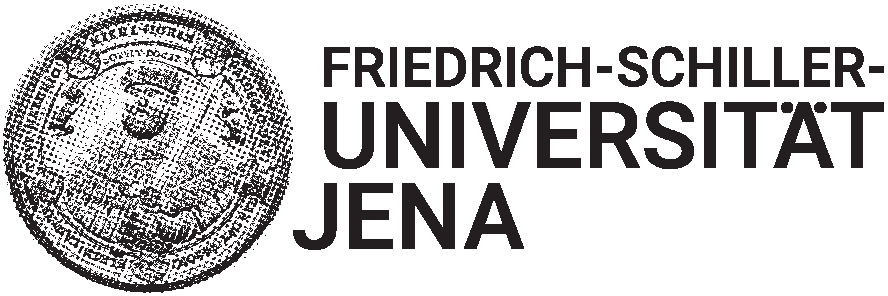
\includegraphics[width=0.75\textwidth]{../UniJena_BildWortMarke_black.pdf}\\[4em]
  \Large
  Ausarbeitung zum Versuch\\[2em]
  \Huge
  Gaslaser\\
  \vspace{2cm}
  \Large
  Martin Beyer und Vanessa Huth\\[2em]
  Abgabe: 30. September 2020\\[2em]
  Betreuer: Dr. Joachim Hein\\[5em]
  \begin{flushleft}
  	Bewertung und Ausarbeitung:\\[2em]
		Protokollführung und Form:\\[1em]
		Ergebnisse, Auswertung und Interpretation:\\[1em]
		Bemerkungen und Hinweise des Betreuers:
  \end{flushleft}
\end{center}
\clearpage

\pagestyle{fancy}
\renewcommand{\headrulewidth}{0pt}
\renewcommand{\footrulewidth}{0.5pt}
\renewcommand{\sectionmark}[1]{\markright{#1}}
\fancyhead[RO,LE]{\textbf{Gaslaser}}
\fancyhead[RE,LO]{\rightmark}
\fancyfoot[LE,RO]{\bfseries\thepage}
\fancyfoot[CO,CE]{Protokoll}
\renewcommand{\headrulewidth}{0.5pt}
\renewcommand{\footrulewidth}{0.5pt}

\setcounter{equation}{0}
\setcounter{figure}{0}

% *********************************************
% ***** KAPITEL 1 *****************************
% *********************************************
\tableofcontents
% \pagenumbering{gobble}% remove page numbering
\newpage
% \pagenumbering{arabic}
\section{Aufgabenstellung} \label{sec:Aufgabenstellung}

\subsection{Messungen der räumlichen Intensitätsverteilung}

\paragraph{Aufgabe 1.1}$~$

Es wird experimentell der Taillenradius $w_0$ für drei verschiedene Resonatorlängen ($L= \SI{0.5}{\metre}, \SI{0.75}{\metre}, \SI{0.9}{\metre}$) bestimmt und mit den theoretischen Vorhersagen verglichen. Dabei werden folgende Methoden benutzt:
\begin{enumerate}
  \item Durch Einbringen eines dünnen Drahtes $(d =\SI{50}{\micro\metre})$ \emph{in den Resonator} werden verschiedene transversale Moden erzwungen. Durch transversales verfahren wird die Differenz der Positionen vermessen, an denen die TEM$_{02}$-Mode erscheint und daraus die Taille $w_0$ berechnet. Es wird eine Fehlerbetrachtung durchgeführt.
  \item Der Bündelradius $w(z)$ \emph{außerhalb des Resonators} wird durch Ausmessen der Knotenlinien der TEM$_{02}$-Mode bestimmt. Daraus wird der Taillenradius $w_0$ unter der Beachtung berechnet, dass der Auskoppelspiegel als plankonkave Linse wirkt. Die Berechnung wird ebenfalls ohne Berücksichtigung des Auskoppelspiegels durchgeführt.
\end{enumerate}

\paragraph{Aufgabe 1.2}$~$

Die Laserleistung in der TEM$_{00}$-Grundmode wird für verschiedene Resonatorlängen und die Leistungen der höheren Moden für eine Resonatorlänge gemessen und interpretiert.

\paragraph{Aufgabe 1.3}$~$

Unter Wahl einer geeigneten Resonatorkonfiguration werden höhere Transversalmoden selektiert und fotografiert. Es werden die Beugungsverluste höherer Transversalmoden gegenüber der TEM$_{00}$-Mode diskutiert und die Frage beantwortet, wie die TEM$_{00}$-Mode sicher erzeugt werden kann.

\subsection{Messungen der spektralen Intensitätsverteilung}

\paragraph{Aufgabe 2.1}$~$

Der Zeitverlauf eines Single-Mode-Lasers SML mit periodisch variierender Resonatorlänge (Wobbelungs-Betrieb) wird mithilfe eines Oszilloskops gemessen. Es wird erklärt, wie auf diese Weise das Spektrum gemessen werden kann. Es wird die Oszillationsbandbreite des SML, der minimal auflösbare Frequenzabstand bestimmt, mit dem Auflösungsvermögen eines Prismenspektrometers verglichen und die Frage beantwortet, welche Längenänderung mit der Anordnung noch messbar ist.

\paragraph{Aufgabe 2.2}$~$

Der Lamb-Dip wird identifiziert, vermessen und die Absenkung im Intensitätsprofil erklärt. Aus der Halbwertsbreite des Lamb-Dip $\Delta v_{LD}$ wird die Größenordnung der homogenen Linienbreite $\Delta v_{HL}$ abgeschätzt und mit der Dopplerbreite $\Delta v_{D}$, sowie der natürlichen Linienbreite des Übergangs verglichen. Das Verstärkungsprofil des He-Ne-Lasers wird skizziert.

\paragraph{Aufgabe 2.3}$~$

Die Lage der Axialmoden des Multi-Mode-Lasers MML wird mit Hilfe eines \emph{optischen Heterodyns} festgestellt. Dafür werden MML und SML derart überlagert, dass sich gut interferieren können. Es wird die zeitliche Konstanz der Axialmoden diskutiert und die Resonatorlänge des MML variiert.

\paragraph{Aufgabe 2.4}$~$

Das Schwebungssignal zwischen den Frequenzen beider Laser wird in Echtzeit (SML ohne Wobbelung) beobachtet und die Größenordnungen der Kurzzeitfluktuationen der Laserfrequenz eines freilaufenden Lasers angegeben.

% *********************************************
% ***** KAPITEL 2 *****************************
% *********************************************
\newpage
\section{Grundlagen} \label{sec:Grundlagen}
Ein Laser besteht aus zwei grundlegenden Elementen, einem verstärkenden Material (aktives Medium) und einem Resonator, welcher im einfachsten Fall aus zwei Spiegeln besteht. Die Verstärkung des Lichtes erfolgt durch stimulierte Emission.

\subsection{Absorption und Emission von Licht}
Nach dem \textsc{Bohr}'schen Atommodell besteht ein Atom aus einem punktförmigen Kern und einer Elektronenhülle, in der sich die Elektronen auf diskreten Bahnen bewegen. Den Bahnen werden Energien zugeordnet, welche in der Summe das Energieniveau des Atoms ergeben. Im Folgenden werden zwei Energieniveaus $E_1$ und $E_2$ betrachtet, deren Besetzungszahlen (Anzahl an Atomen pro Volumen) mit $N_1$ und $N_2$ bezeichnet werden. Die Änderung des Energieniveaus von Zustand $E_1$ zu $E_2$ kann durch Emission oder Absorption von Photonen der Energie
\begin{align}
  h\nu = |E_2 - E_1|
\end{align}
erreicht werden, vorausgesetzt, der Übergang ist nach den Auswahlregeln der Quantenmechanik erlaubt.

\begin{figure}[htp]
  \centering
  \begin{tikzpicture}[every text node part/.style={align=center}]
    \draw[thick] (-1,0)node[left]{$E_1$} -- (1,0);
    \draw[thick] (-1,1.5)node[left]{$E_2$} -- (1,1.5);
    \draw[thick] (-1,2)node[left]{$E_3$} -- (1,2);
    \node (A) at (0,2.5){Absorption};
    \draw[thick, ->] (0,0) -- (0,1.5);
    \draw[->,red, decorate, decoration={snake,amplitude=.4mm,segment length=2mm,post length=0.5mm}] (-1.5,.75) --node[above]{$h\nu$} (0,.75);
    \shadedraw[draw=black, thick, top color = black!30!white, bottom color=black!50!white] (0,0) circle (.15cm);

    \begin{scope}[shift={(4,0)}]
      \draw[thick] (-1,0)node[left]{$E_1$} -- (1,0);
      \draw[thick] (-1,1.5)node[left]{$E_2$} -- (1,1.5);
      \draw[thick] (-1,2)node[left]{$E_3$} -- (1,2);
      \node (A) at (0,2.7){spontane\\Emission};
      \draw[thick, <-] (0,0) -- (0,1.5);
      \draw[->,red, decorate, decoration={snake,amplitude=.4mm,segment length=2mm,post length=0.5mm}] (0,.75) -- (1.5,1);
      \shadedraw[draw=black, thick, top color = black!30!white, bottom color=black!50!white] (0,1.5) circle (.15cm);
    \end{scope}

    \begin{scope}[shift={(8,0)}]
      \draw[thick] (-1,0)node[left]{$E_1$} -- (1,0);
      \draw[thick] (-1,1.5)node[left]{$E_2$} -- (1,1.5);
      \draw[thick] (-1,2)node[left]{$E_3$} -- (1,2);
      \node (A) at (0,2.7){induzierte\\Emission};
      \draw[thick, <-] (0,0) -- (0,1.5);
      \draw[->,red, decorate, decoration={snake,amplitude=.4mm,segment length=2mm,post length=0.5mm}] (-1.5,.75) -- (0,.75);
      \draw[->,red, decorate, decoration={snake,amplitude=.4mm,segment length=2mm,post length=0.5mm}] (0,1) -- (1.5,1);
      \draw[->,red, decorate, decoration={snake,amplitude=.4mm,segment length=2mm,post length=0.5mm}] (0,.5) -- (1.5,.5);
      \shadedraw[draw=black, thick, top color = black!30!white, bottom color=black!50!white] (0,1.5) circle (.15cm);
    \end{scope}
  \end{tikzpicture}
  \caption{Schematische Darstellung von Absorptions- und Emissionsprozessen nach~\cite{Eichler}.}
  \label{fig:Absorption_Emission}
\end{figure}


Befindet sich das Atom in einem angeregten Zustand $E_2$, dann kann es unter Emission eines Photons in den niedrigeren Zustand $E_1$ fallen (siehe Abbildung~\ref{fig:Absorption_Emission}). Erfolgen diese Emissionen ohne jeglichen Einfluss von außen, wird von \emph{spontaner} Emission gesprochen. Das ausgesendete Licht steht untereinander in keiner festen Phasenbeziehung, Ausbreitungsrichtung oder Polarisation.

Die Rate der Emissionsprozesse ist proportional zur Anzahl an Atomen im angeregten Zustand $N_2$. Bei der \emph{induzierten} Emission, wird das angeregte Atom durch ein äußeres Photon zur Emission gezwungen, wobei zwei identische Photonen entstehen. Die Rate der induzierten Emission ist zusätzlich noch proportional zur spektralen Energiedichte $u(\nu)$ des Strahlungsfeldes. Diese Zusammenhänge lassen sich mithilfe folgender Differentialgleichungen mathematisch formulieren:
\begin{align}
  \dv{N_1}{t} &= - B_{12} N_1 u(\nu) & \text{Absorption}\\
  \dv{N_2}{t} &= - A_{12} N_2 u(\nu) & \text{spontane Emission}\\
  \dv{N_2}{t} &= - B_{21} N_2 u(\nu) & \text{induzierte Emission}.
  \label{equ:Ratengleichungen}
\end{align}
Die Proportionalitätskonstanten stellen hierbei die Einsteinkoeffizienten dar. Im thermodynamischen Gleichgewicht ergibt sich eine Balance zwischen Absorption und Emission:
\begin{align}
  N_2 = N_1 \exp\qty(-\frac{h\nu}{k_B T}).
\end{align}
Wird damit nun die spektrale Energiedichte $u(\nu)$ bestimmt und mit der \textsc{Planck}'schen Strahlungsformel verglichen, ergibt sich
\begin{align}
  \frac{A_{21}}{B_{21}} = \frac{8\pi h \nu^3}{c^3} \quad \text{und} \quad B_{12} = B_{21}.\label{equ:Einsteinkoeffizienten}
\end{align}
Es ergibt sich somit eine Gleichheit der Koeffizienten der Absorption und induzierten Emission. Zudem ist für hohe Frequenzen die spontane Emission $A_{21}$ dominant gegenüber der induzierten Emission $B_{21}$, was den Grund darstellt, warum es schwierig ist, UV-Laser zu konstruieren.

\subsection{Linienbreite}
Bei der Absorption oder Emission elektromagnetischer Strahlung bei einem Übergang zwischen zwei Energieniveaus ist die Frequenz nicht streng monochromatisch.

\paragraph{Natürliche Linienbreite}$~$

Die natürliche Linienbreite ist eine Folge der endlichen Lebensdauer der Zustände bei der spontanen Emission. Nach der \textsc{Heisenberg}'schen Unschärferelation, ergibt sich die Energieunschärfe des Übergangs zu
\begin{align}
  \Delta \nu_\text{nat.} = \frac{1}{2\pi \tau},
\end{align}
wobei die Lebensdauer $\tau$ für den im Versuch verwendeten He-Ne-Laser $\tau = \SI{10}{\nano\second}$ beträgt, was einer natürlichen Linienbreite von \SI{16}{\mega\hertz} entspricht. Die Form der Emissionslinie lässt sich mithilfe des Oszillatormodells der Elektronen herleiten und ergibt als Spektrum ein Lorentz-Profil.

\paragraph{Stoßverbreiterung}$~$

Zusätzlich zur endlichen Lebensdauer können elastische Stöße zwischen den Gasteilchen auftreten. Diese Verbreiterung wird \emph{homogen} genannt, da sie alle Atome gleichermaßen betrifft. Da die Zahl der Stöße druckabhängig ist, wird ebenfalls von Stoßverbreiterung gesprochen. Die Halbwertsbreite ergibt sich analog zu
\begin{align}
    \Delta \nu_\text{St.} = \frac{1}{2\pi \tau_\text{St.}},
\end{align}
wobei $\tau_\text{St.}$ die mittlere Zeit zwischen zwei Stößen angibt. Für den He-Ne-Laser ergibt sich damit einer Verbreiterung von \SI{50}{\mega\hertz\per\milli\bar}.
Im Festkörper beruht die Stoßverbreiterung auf der Wechselwirkung von Phonon.

\paragraph{Dopplerverbreiterung}$~$

Bewegt sich das angeregte Atom mit der Geschwindigkeit $\bm{v}$, so wird die Mittenfrequenz $\nu_0$ um einen Betrag verschoben, welcher der Dopplerverschiebung einer bewegten Quelle entspricht. Es handelt sich hierbei um eine inhomogene Verbreiterung, welche sich in einem gaußförmigen Linienprofil zeigt. Für den im Versuch benutzten Übergang beträgt die Dopplerverbreiterung \SI{1500}{\mega\hertz} und stellt die dominante Größe der Verbreiterung dar.

\subsection{Die Laserbedingungen}
Das Prinzip des Lasers ist es, Licht zu verstärken. Damit dies möglich wird, bedarf es eines Mediums, welches genau das gewährleistet, das sogenannte \textit{aktive Medium}. Verstärkung tritt auf, wenn für die Photonenzahldichte $q$
\begin{align}
  \dv{q}{t} \geq 0
  \label{equ:Photonenzahldichte}
\end{align}
gilt. Um einen Ausdruck für die Photonenzahldichte herzuleiten, stellen wir die Bilanz aus den das Laserniveau verlassenden, also induziert emittierten und den zum Laserniveau hinzukommenden, also den absorbierten Photonen auf. Die spontane Emission wird hier vernachlässigt. Mit den oben hergeleiteten Formeln \eqref{equ:Ratengleichungen} ergibt sich für die Photonenzahldichte
\begin{align}
    \dv{q}{t}=-\dv{N_2}{t}+\dv{N_1}{t}=u(\nu)(B_{21}N_2-B_{12}N_1)=u(\nu)B_21(N_2-N1)
\end{align}
Da weiterhin Gleichung \eqref{equ:Photonenzahldichte} gelten muss, bedeutet das, eine Verstärkung tritt auf, wenn
\begin{align}
  \boxed{N_2 ß\geq N_1 \qquad \emph{1. Laserbedingung}}
\end{align}
also wenn sich mehr Atome im angeregten, als im Grundniveau befinden. Im thermischen Gleichgewicht gilt genau das Inverse, nämlich $N_1 \geq N_2$, weshalb dieser Zustand als \textit{Besetzungsinversion} bezeichnet wird. Ihn erreicht man also nicht durch thermische Anregungen, egal, wie hoch man die Temperaturen wählt, sondern nur durch spezielle Anregungsvorgänge- das sogenannte \textit{Pumpen}.\\
Die zur Anregung nötige Energie kann auf unterschiedliche Wege zugeführt werden, was zur Unterscheidung der unterschiedlichen Lasertypen führt.
\begin{itemize}
  \item optisch gepumpte Laser (Anregung durch Blitzlampe, kontinuierliche Lampe, Laser, Leuchtdiode)
  \item elektronenstrahlgepumpte Laser
  \item Gasentladungslaser
  \item Injektionslaser (Anregung durch Stromdurchgang in Halbleiter)
  \item chemische Laser(Anregung durch chemische Reaktion)
  \item gasdynamische Laser (Inversionserzeugung durch Expansion eines heißen Gases)
  \item nuklear gepumpte Laser
\end{itemize}

Die Besetzungsinversion wird dabei grundsätzlich theoretisch immer gleich erzielt. Es wird zwischen 2-Niveau, 3-Niveau und 4-Niveau-System unterschieden, wobei bei 2-Niveau-Systemen aufgrund Gleichung \eqref{equ:Einsteinkoeffizienten} die Erzeugung einer Inversion durch optisches Pumpen nicht möglich ist. Bei einem 3-Niveau-System gibt es ein Hilfsniveau $E_3$ welches sich dadurch auszeichnet, dass es ein breites Absorptionsband, dass Licht einer Blitzlampe gut absorbieren kann und dann schnell in Niveau $E_2$ zerfällt. Entscheidender Nachteil ist, dass hier eine hohe Pumprate nötig ist. Dieses Problem löst das 4-Niveau-System, indem hier der Laserübergang nicht zum Grundzustand sondern zu einem Zwischenzustand erfolgt. \\
Um den Lichtverstärker zum Oszillator - dem Laser-zu machen, bedienen wir uns einem Prinzip der Elektronik, der Rückkopplung: Ein Teil der verstärkten Ausgangsstrahlung wird wieder in das System zurückgeführt. Dies wird realisiert durch zwei Spiegel rechts und links vom aktiven Medium. Sie bilden den \textit{Resonator}. Entscheidend für die Entstehung der Oszillation ist, dass die Verluste pro Umlauf geringer sind, als die Verstärkung pro Umlauf. Für die Verstärkung nach einem doppelten Durchlauf wird in Analogie zum \textsc{Lambert-Beer}'schen Gesetz für die Absorption
\begin{align}
  I(2L)=I(0)\cdot \exp{g2L} \qquad \text{mit} g = B_{21} \frac{h\nu}{c} (N_2-N_1)
\end{align}
gefunden. Gleichzeitig kann, wenn alle Verluste (Spiegeltransmission, Streuung, Beugung, Absorption) in einem Verlustkoeffizienten $\kappa$ zusammengefasst werden, die Bedingung, dass die Verstärkung die die Verluste nach einem Umlauf kompensiert, als
\begin{align}
  I(0)=I(2L)\cdot \exp{-\kappa}
\end{align}
Da der Laser wie eingangs beschrieben, nur dann oszillieren kann, wenn die Verstärkung größer oder gleich den Verlusten pro Umlauf ist, ergibt sich so die \textit{zweite Laserbedingung}
\begin{align}
  \boxed{\sigma_{21}(N_2-N_1)\cdot2L \geq \kappa}
  \label{equ:zweiteLB}
\end{align}
Die Erfüllung von \eqref{equ:zweiteLB} wird durch die Lage der zweiten Verlustlinie charakterisiert.


\subsection{Der Inversionsabbau und Lamb-Dip}
 Der Laserprozess läuft folgendermaßen ab: In der zunächst eintretenden Einschwingphase liegen kleine Intensitäten vor. Bei diesen tritt eine exponentielle Verstärkung auf. Bei höheren Intensitäten wird die Inversion und damit die Verstärkung durch induzierte Emission zunehmend abgebaut. Bei konstantem Pumpen kommt es durch diesen zunehmenden Inversionsabbau zu einem Gleichgewichtszustand, der sogenannten Sättigung der Verstärkung. Die Besetzungsinversion wird dabei bis zur Verlustlinie abgebaut.

Bei homogener Linienverbreiterung können alle invertierten Atome mit dem Strahlungsfeld bzw. der Mode wechselwirken, so kann sie von allen Atomen ihre Verstärkung beziehen, der Abbau erfolgt, wie in Abbildung \ref{fig:homogen} gleichermaßen.

\begin{figure}[htp]
    \centering
        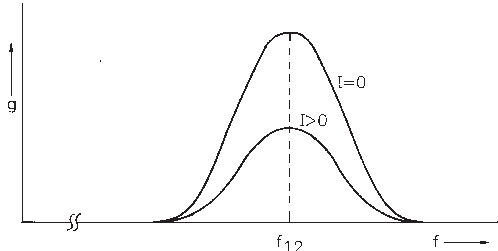
\includegraphics[width=0.5\textwidth]{Bilder/Saettigung_homogen.pdf}
    \caption{homogene Sättigung des Linienprofils}
    \label{fig:homogen}
\end{figure}

Bei inhomogener Linienverbreiterung kann das Strahlungsfeld hingegen nur mit bestimmten Atomen wechselwirken, die Mode kann also nur einen Teil der invertierten Atome abbauen, nämlich die, die aufgrund der homogenen Linienbreite trotz des Dopplereffekts noch die Resonatorfrequenz haben. Die Verstärkung wird dann nur in einem engen Frequenzbereich um die Frequenz der wechselwirkenden Atome abgebaut, was in Abbildung \ref{fig:inhomogen} visualisiert ist. Aufgrund des sich ergebenden Bildes im Verstärkungsprofil spricht man vom ``hole burning''.

\begin{figure}[htp]
    \centering
        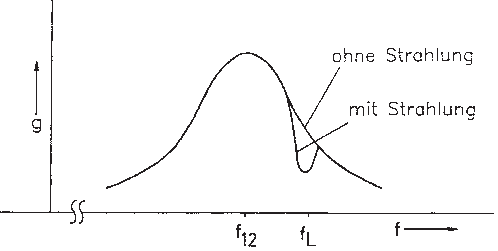
\includegraphics[width=0.5\textwidth]{Bilder/Saettigung_inhomogen.pdf}
    \caption{Sättigung bei einer inhomogenen Linie}
    \label{fig:inhomogen}
\end{figure}

Aufgrund des Dopplereffekts können beim Gaslaser nur Atome wechselwirken, die sich gerade mit der passenden Geschwindigkeit $\pm v_z$ in z-Richtung (Laserachsenrichtung) bewegen, sodass ihre Frequenz gerade der Resonatorfrequenz entspricht.  Symmetrisch um die Null kommt es bei $pm v_z$ zu einer Eindellung des Verstärkungsprofil bei der negativen sowie bei der positiven Geschwindigkeit. Zur Ausgangsleistung tragen hier zwei Gruppen von Atomen bei, nämlich die, die sich mit der Geschwindigkeit $v_z$ bewegen, sie sorgen für eine Emission des Lichts in positive z-Richtung und die, die sich mit der Geschwindigkeit $-v_z$ bewegen, sie sorgen für eine Emission des Lichts in negative z-Richtung, haben aber die gleiche Frequenz. Ist aber die Resonatorfrequenz gleich der Resonanzfrequenz des optischen Übergangs, verschiebt man die Frequenz also zur Linienmitte, kommt es zum Überlappen der beiden Löcher. Jetzt tragen nur noch Atome mit $v_z = 0$, also viel weniger, als in den anderen Fällen, zur Verstärkung bei. Es kommt deshalb zur Eindellung der Intensität. Da hier alle Atome $v_z = 0 $ haben, tritt auch kein Dopplereffekt mehr auf, weshalb die Eindellung bei jenem $\nu$ nur noch homogen verbreitert ist und keine Dopplerverbreiterung aufweist, weshalb gilt
\begin{align}
  \Delta \nu_{HL} = \Delta \nu_{LD}
\end{align}


\subsubsection{Moden}
Im Laser treten longitudinale und transversale Moden  auf. Longitudinale Moden sind die Eigenschwingungen des Resonators und entsprechen stehenden Wellen. Für sie gilt also
\begin{align}
  n L = k_i \frac{\lambda}{2_i}
\end{align}
wobei $k_i$ die Anzahl der stehenden Halbwellen und $\lambda_i$ die Wellenlänge der i-ten Mode entsprechen, n ist der Brechungsindex und L die Länge des Resonators. Im Resonator werden jetzt nicht wie noch im Lichtverstärker ein Kontinuum von Frequenzen unter dem Verstärkungsprofil verstärkt, sondern nur die Eigenfrequenzen des Resonators erfahren eine Verstärkung. Die Selbstoszillation der Eigenfrequenzen ist nur möglich, da die induzierte Emission die Eigenschaften der Phasenstarre, der Frequenzidentität und der Polarisationserhaltung mitbringt. Wird die Frequenzdifferenz zwischen zwei stehenden Wellen mit k und k+1 betrachtet, ergibt sich der Frequenzabstand zwischen zwei Axialmoden zu
\begin{align}
  \Delta \nu = \frac{c}{2nL}
\end{align}
Transversalmoden treten durch eine leichte Phasenverschiebung bei der Reflexion an den Resonatorspiegeln, die sich in einer kleinen Frequenzänderung ausdrückt. Jeweils gleiche transversale Moden haben aber ebenfalls einen konstanten Frequenzabstand, wie die longitudinalen.

\subsection{Gaußsche Strahlenoptik}
Um die Eigenschaften der Strahlenoptik, welche die Ausbreitung von Licht in optischen Systemen beschreibt, mit der Wellenoptik zu vereinen, werden Gaußstrahlen eingeführt. Sie stellen eine paraxiale Lösung der \textsc{Helmholtz}-Gleichung dar und eignen sich zur Beschreibung der Ausbreitung kohärenter Laserstrahlen. Ein kollimierter Laserstrahl propagiert gerichtet in einem homogenen Material. Aufgrund von Dispersionseffekten divergiert der Gaußstrahl jedoch. Der Gaußstrahl wird im Gegensatz zu einer ebenen Welle modelliert mit einer gaußförmig verlaufenden Amplitude entlang axialer Richtung. Damit lässt sich die komplexe Amplitude des Gaußstrahles schreiben als~\cite{Saleh}
\begin{align}
  E(\bm{r}) = E_0 \frac{W_0}{W(z)} \exp\qty(-\frac{\varrho}{W(Z)})^2 \exp[-\mathrm{i}\qty(kz + k \frac{\varrho^2}{2R(z)}+ \arctan\qty(\frac{z}{z_R})^2)],
\end{align}
wobei $\varrho^2 = x^2 + y^2$ die transversale Koordinate beschreibt. Der Ausdruck $W(z)$ beschreibt den Radius des Strahls entlang der Ausbreitungsrichtung $z$ und $R(z)$ definiert den Krümmungsradius der Wellenfront aufgrund der Divergenz des Strahls. Sie sind definiert als
\begin{align}\label{eqn:Strahlradius_Krümmung}
  W(z) = W_0 \sqrt{1+\qty(\frac{z}{z_R})^2}, \qquad R(Z) = z \qty[1+\qty(\frac{z_R}{z})^2]
\end{align}
Die Größe $z_R$ wird \textsc{Rayleigh}-Länge genannt und beschreibt den Abstand zum Fokuspunkt ($z=0$) bei dem die Leistung der Strahlungsachse auf die Hälfte des Maximalwertes abgefallen ist. Es ergibt sich
\begin{align}\label{eqn:z_r}
  z_R = \frac{\pi W_0^2}{\lambda}.
\end{align}

\begin{figure}[htp]
  \centering
  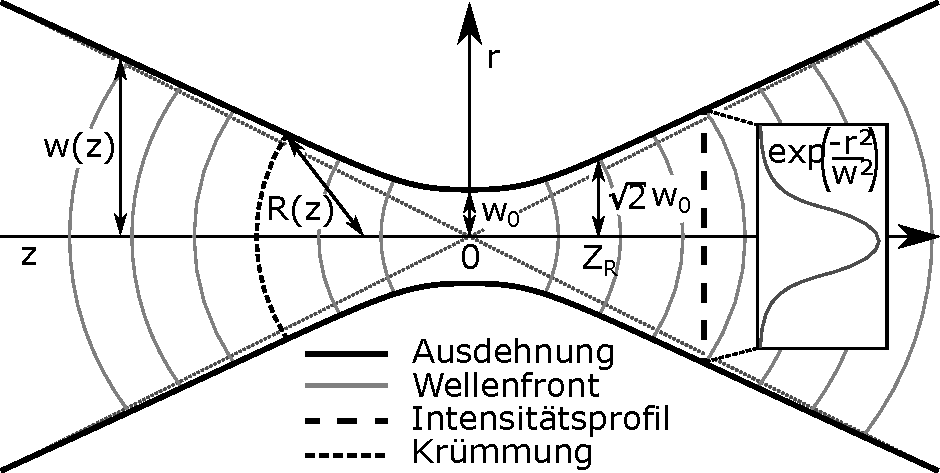
\includegraphics[width=.7\textwidth]{Bilder/Gauss_Strahl.pdf}
  \caption{Schematische Darstellung eines Gaußstrahls mit Abmessungen, Strahlbegrenzung, Wellenfronten und Intensitätsprofil. Von Aleph - Eigenes Werk, CC BY-SA 2.5, \url{https://commons.wikimedia.org/w/index.php?curid=3807143}}
  \label{fig:Gauss_Strahl}
\end{figure}

\subsubsection{Strahlparameter und Matrizenoptik}
Wie in der Strahlenoptik lässt sich die Ausbreitung eines Gaußstrahls mithilfe von Matrizen beschreiben. Dabei kann die Propagation im freien Raum und durch optische Bauelemente bequem durch eine Matrix beschrieben werden. Diese ist im Folgenden für verschiedene Optische Elemente dargelegt~\cite{Peschel}:
\begin{align}
  M &= \begin{pmatrix}
    1 & L \\ 0 & 1
\end{pmatrix} & \text{Freiraum der Länge }L \label{eqn:Matrix_Freiraum}\\
  M &= \begin{pmatrix}
  1 & 0 \\ -\frac{1}{f} & 1
\end{pmatrix} & \text{Linse mit Brennweite }f \label{eqn:Matrix_Brennweite}\\
  M &= \begin{pmatrix}
  1 & 0 \\ \frac{2}{R} & 1
\end{pmatrix} & \text{Spiegel mit Krümmungsradius }R.
\end{align}

Zur vereinfachten Beschreibung des Gaußstrahls werden seine Kenngrößen zu einem komplexen Parameter $q$ zusammengefasst
\begin{align}\label{eqn:q-Parameter}
  q = z_F - \mathrm{i} z_r \qquad \frac{1}{q} = \frac{1}{R(z)} + \mathrm{i}\frac{\lambda}{\pi}\frac{1}{W(z)^2}
\end{align}
Dabei bezeichnet $z_F$ den Abstand zum Fokus (Strahltaille) und $z_r$ die \textsc{Rayleigh}-Länge. Für ein optisches System mit der Transfermatrix $M$ ergibt sich der neue $q$-Parameter wie folgt:
\begin{align}\label{eqn:Transfermatrix}
  M = \begin{pmatrix}
    A & B \\ C & D
\end{pmatrix}, \qquad q_+ = \frac{A q_- + B}{C q_- + D}.
\end{align}

\subsubsection{Resonatortypen}
Ein optischer Resonator besteht typischerweise aus zwei Spiegeln und wird charakterisiert durch die Resonatorlänge $L$ und den Krümmungsradius $R$ der Spiegel. Der Umlauf im Resonator lässt sich durch eine Matrix beschreiben. Damit sich ein Gaußstrahl auf sich selbst abbildet, muss $q_+ = q_- = q$ gelten. Das führt mit Gleichung~\eqref{eqn:Transfermatrix} auf eine quadratische Gleichung, deren Lösung für einen klassischen Laserresonator mit zwei Hohlspiegeln durch folgende Beziehung gegeben ist:
\begin{align}\label{eqn:Resonatorformel}
  |2g_1 g_2 -1 | < 1, \qquad g_x = 1 + \frac{L}{R_x}.
\end{align}
Dabei bezeichnen $g_1$ und $g_2$ die Spiegelparameter des Laserresonators. Ein Resonator ist also nur dann stabil, wenn~\eqref{eqn:Resonatorformel} gilt. Die Bereiche, für die ein stabiler Resonator möglich ist, sind in Abbildung~\ref{fig:Stabilität} dargestellt.

\input{Bilder/Stabilität.tex}

Hinsichtlich der Krümmungsradien lassen sich drei wichtige Typen unterscheiden:

\begin{enumerate}[label=\Alph*)]
  \item \emph{Planspiegelresonator} (Fabry-Perot-Resonator): Hier sind zwei planare Spiegel im Abstand $L$ angeordnet. Die transversale Ausdehnung des Strahls bestimmt das aktive Medium oder der Spiegeldurchmesser. Es bildet sich eine Feldverteilung, die $\cos^2$-förmig variiert entlang des Querschnitts.
  \item \emph{Konfokaler Resonator}: Hier bildet sich ohne Einfluss begrenzender Aperturen eine begrenzte, gaußförmige Feldverteilung aus.
  \item \emph{Konzentrischer Resonator}: Hier liegen die Krümmungsmittelpunkte im gleichen Punkt, die Spiegel weisen den Abstand $L=2R$ auf. Die transversale Ausdehnung der Feldverteilung hängt nur von den begrenzenden Aperturen ab.
\end{enumerate}
\FloatBarrier
\subsection{Der Helium-Neon-Laser}
Der Helium-Neon-Laser ist ein Gaslaser, der als aktives Medium ein He-Ne-Gasgemisch benutzt. Das Helium wird durch Elektronenstöße angeregt und gibt seine Energie durch Stöße zweiter Art an das Neonatom ab, in welchem dann die Laserübergänge passieren. Wobei ein Stoß zweiter Art folgenden Prozess benennt:
\begin{align}
  \text{He}* + \text{Ne} \Rightarrow \text{He}+\text{Ne}*+\Delta E
\end{align}
Das Termschema des He-Ne ist in Abbildung \ref{fig:Termschema} zu sehen.

\begin{figure}[htp]
  \centering
  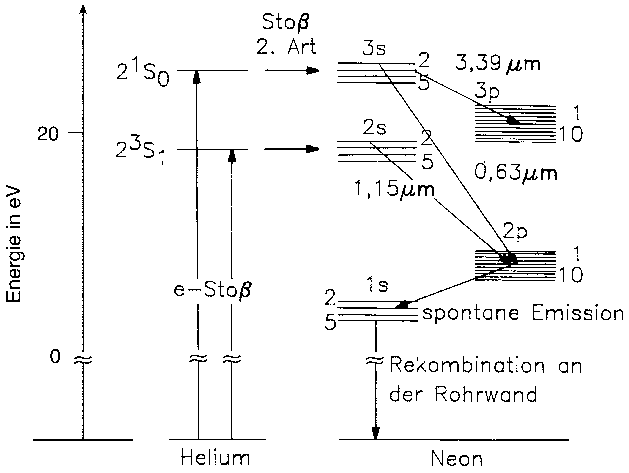
\includegraphics[width=0.5\textwidth]{Bilder/HeNe-Termschema.pdf}
  \caption{Thermschema des He-Ne-Lasers}
  \label{fig:Termschema}
\end{figure}

Die resonante Übertragung der Energie von He auf Neon ist der hauptsächliche Pumpvorgang. Der für den Versuch relevante Übergang ist der 3s $\rightarrow$ 2p, durch den die rote Linie bei \SI{632,8}{\nano\meter} entsteht. Da die Entleerung des 1s Niveaus hauptsächlich durch Stöße mit der Wand passiert, wird beim Bau der Röhren auf ein dünnes Rohr geachtet, was die Ausgangsleistung der Laser auf \SI{10}{\milli\watt} beschränkt.

\begin{figure}[htp]
  \centering
  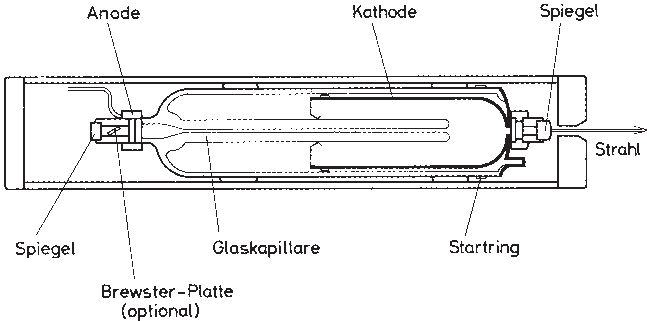
\includegraphics[width=0.7\textwidth]{Bilder/HeNe-Laser_Aufbau.pdf}
  \caption{schematischer Aufbau eines He-Ne-Lasers}
  \label{fig:Aufbau}
\end{figure}

Der Aufbau des He-Ne-Lasers ist in Abbildung \ref{fig:Aufbau} dargestellt. Die Elektronen, die für die Anregung des Heliums nötig sind, entstehen durch Gasentladung. Hierfür ist eine Hochspannung im Bereich \SI{2}{\kilo\volt} erforderlich. Technisch wichtig ist die bereits oben diskutierte kleine Kapillardurchmesser, sowie die Notwendigkeit von Spiegeln mit hohen Reflexionsvermögen, da unter realistischen Bedingungen nur eine Verstärkung von g$=\SI{0,1}{\per\meter}$ erzielt werden kann. Außerdem entscheidend ist für die Selektion einer Polarisationsrichtig die Verwendung von unter dem Brewster-Winkel geneigten Fenstern. Diese bewirken, dass nur senkrecht polarisiertes Licht die Kapillare verlässt. Typischerweise wird, wie auch im Versuch, an einem Spiegel ausgekoppelt, der z.B. ein Reflexionsvermögen von \SI{98}{\percent} aufweist. Das Mischungsverhältnis zwischen beiden Gasen bestimmt die emittierte Wellenlänge. Für die verwendete Rotlinie wird ein Verhältnis von 5:1 gewählt.

% *********************************************
% ***** KAPITEL 4 *****************************
% *********************************************
\newpage
\section{Ergebnisse und Diskussion}\label{sec:ErgebnisseUndDiskussion}

\subsection{Messungen der räumlichen Intensitätsverteilung}

Zur Vorbereitung der Aufgabe wird die Größe der Strahltaille $w_0$ für verschiedene Längen $0 < L < 2R$ eines symmetrischen Resonators $L = \SI{50}{\centi\metre}$ berechnet. Hierfür wird die Tatsache genutzt, dass der Krümmungsradius des Strahlenbündels am Ort des Spiegels dessen Krümmungsradius entspricht. Es ergibt sich mithilfe von~\eqref{eqn:Strahlradius_Krümmung}
\begin{align}
  R\qty(\frac{L}{2}) \overset{\eqref{eqn:Strahlradius_Krümmung} }{=} \frac{L}{2} \qty(\frac{4 z_r^2}{L^2} + 1) \overset{!}{=} R.
\end{align}
Für die \textsc{Rayleigh}-Länge und folglich auch die Strahltaille $w_0$ ergibt sich dann
\begin{align}\label{eqn:Strahltaille}
  z_r^2 = \frac{R \cdot L}{2} - \frac{L^2}{4} \quad \overset{\eqref{eqn:z_r}}{\Rightarrow} w_0(L) = \sqrt{\frac{\lambda}{\pi} z_r(L)} = \sqrt{\frac{\lambda}{2\pi}\sqrt{L(2R - L)}}.
\end{align}
Der sich ergebende Verlauf der Strahltaille als Funktion der Resonatorlänge ist in Abbildung~\ref{fig:Strahltaille_Theorie} dargestellt.

\begin{figure}[htp]
  \centering
  \begin{tikzpicture}[every text node part/.style={align=center}]
    \begin{axis}[disabledatascaling, width=0.95\textwidth, height=6cm, ylabel=Strahltaille $z_r$ in \si{\micro\metre}, xlabel=Resonatorlänge $L$ in \si{\metre}, xmin=0, xmax=1, ymin = 0, samples = 200, domain=0:1]
      \addplot[blue, thick] {(2*0.5*x-x^2)^(1/4)*(0.6328/(2*pi))^(1/2)*1000};
      \draw[<-] (.5,10) -- (.5,50)node[above]{Konfokaler\\ Resonator};
      \draw[<-] (.01,10) -- (.1,50)node[above]{Fabry Perot\\ Resonator};
      \draw[<-] (.99,10) -- (.9,50)node[above]{Konzentrischer\\ Resonator};
    \end{axis}
\end{tikzpicture}
  \caption{Radius der Strahltaille $z_r$ als Funktion der Resonatorlänge $L$ eines symmetrischen Resonators mit Krümmungsradius $R=\SI{0.5}{\metre}$ der Spiegel.}
  \label{fig:Strahltaille_Theorie}
\end{figure}


Es zeigt sich, dass für $L = 2R = \SI{1}{\metre}$ der konfokale Resonator in den konzentrischen übergeht und die Strahltaille $w_0$ gegen Null läuft. Da die Strahldivergenz $\theta$ proportional zur inversen Strahltaille ist, geht hier die Strahldivergenz gegen unendlich und der Resonator wird instabil. Für den Fall planarer Spiegel bei $L/R = 0$ tritt unendliche Strahldivergenz ebenfalls auf. Im Fall des konfokalen Resonators ist der Einfluss einer Aperturblende geringer als im konzentrischen Resonator, da hier die transversale Feldverteilung bereits durch den Resonatoraufbau begrenzt wird.

\subsubsection{Bestimmung des Bündelradius und der Strahltaille}

Um den Bündelradius $w(z)$ zu bestimmen, werden die Knotenlinien der TEM$_{02}$ Mode ausgemessen. Entlang der $y$-Achse bei $x=0$ gilt dann für das elektrische Feld der zweiten transversalen Mode~\cite{Eichler}
\begin{align}\label{eqn:3.TEM02}
  E_{02}(0,y) = H_0(0) H_2(\xi) \exp\qty(-\frac{\xi^2}{2}), \quad \text{mit} \quad \xi = \frac{x\sqrt{2}}{w(z)}.
\end{align}
Die Funktionen $H_m(\xi)$ bezeichnen die Hermite-Polynome, wobei $H_1(\xi) = 1$ und $H_2(\xi) = 4\xi^2- 2$ gilt. Die Nullstellen der Intensität bzw. von~\eqref{eqn:3.TEM02} ergeben sich dann mit der Nullstelle des zweiten Hermite-Polynoms
\begin{align}
  E_{02}(0,y) \overset{!}{=} 0, \quad \Rightarrow \xi = \pm \frac{1}{\sqrt{2}} = \frac{y \sqrt{2}}{w(z)}.
\end{align}
Damit folgt direkt $w(z) = 2y$. Somit ergibt sich, dass der Abstand der Nullstellen der TEM$_{02}$-Mode mit der Bündelbreite $w(z)$ übereinstimmt. Die TEM$_{02}$-Mode kann erzwungen werden, indem ein dünner Draht in den Resonator platziert wird. Wird dieser nun in einer Nullstelle einer Mode positioniert, so bleibt die Feldverteilung dieser Mode unbeeinflusst und alle anderen Moden können ausgeblendet werden. Der durch die Messung ermittelte Radius $w(z)$ lässt sich nun angeben, in beide Gleichungen aus~\eqref{eqn:Strahlradius_Krümmung} ineinander eingesetzt werden. Für einen festen Bündelradius $w(z)$ ergibt sich die Breite der Strahltaille zu~\cite{Anleitung}
\begin{align}\label{eqn:Strahltaille_Experimentell}
  w_0(w,z) = \sqrt{\frac{1}{2}} \sqrt{w^2 \pm \sqrt{w^4-\frac{4z^2 \lambda^2}{\pi^2}}}.
\end{align}
Es muss jedoch noch diskutiert werden, welche Lösung zur Berechnung der Strahltaille verwendet werden muss. Dafür wird eine geometrische Abschätzung durchgeführt. Das Strahlbündel hat bei $z = z_r$ die Ausdehnung $w_0 \sqrt{2}$, wie Abbildung~\ref{fig:Gauss_Strahl} zeigt. Wird $w(z)$ außerhalb der \textsc{Rayleigh}-Länge $z_r$ gemessen, dann ist $w_0 \sqrt{2} < w(z)$ und es muss das Minus beim Vorzeichen gewählt werden. Für $z < z_r$ wird dann das positive Vorzeichen der Wurzel gewählt. Im konfokalen Resonator gilt $R=L$, somit liegt nach Gleichung~\eqref{eqn:Strahltaille} die \textsc{Rayleigh}-Länge bei $z = L/2$, weshalb in diesem Aufbau immer das positive Vorzeichen gewählt wird. Für die anderen Resonatorlängen wird die \textsc{Rayleigh}-Länge mit der Position des Drahtes verglichen, um zu entscheiden, welche Lösung gewählt werden muss.

\begin{figure}[htp]
  \centering
  \begin{tikzpicture}[scale=0.9]

    \shadedraw[top color =black!20!white, bottom color=black!10!white, middle color=black!60!white] (-1.5,0) rectangle (8,0.3);
    \filldraw[thick, draw = black, fill=black!30!white] (-6.5,0) rectangle (8.5,-.3);

    \shade[top color=white, bottom color=red] (3.125,1.5) parabola bend (3.125,1.55) (-1.17,1.65) -- (-1.17,1.5);
    \shade[top color=red, bottom color=white] (3.125,1.5) parabola bend (3.125,1.45) (-1.17,1.35) -- (-1.17,1.5);
    \shade[top color=white, bottom color=red] (3.125,1.5) parabola bend (3.125,1.55) (7.18,1.65) -- (7.18,1.5);
    \shade[top color=red, bottom color=white] (3.125,1.5) parabola bend (3.125,1.45) (7.18,1.35) -- (7.18,1.5);
    \filldraw[draw=black, fill=gray] (-6,0) rectangle +(0.25,0.5);
    \filldraw[draw=black, fill=black!20!white] (-6+0.05,0.5) rectangle +(0.15,0.5);
    \draw[very thick] (-6+0.125,1) -- +(0,2);
    \filldraw[draw=black, fill=gray] (7.5,0) rectangle +(0.25,0.5);
    \filldraw[draw=black, fill=black!20!white] (7.5+0.05,0.5) rectangle +(0.15,0.5);
    \draw[very thick] (7.5+0.125,1) -- +(0,2);

    \filldraw[draw=black, fill=gray] (-1.25,0) rectangle +(0.25,0.5);
    \filldraw[draw=black, fill=black!20!white] (-1.25+0.05,0.5) rectangle +(0.15,0.5);
    \draw[very thick] (-1.25+0.125,1) arc (190:170:3-0.125);

    \filldraw[draw=black, fill=gray] (2.5,0) rectangle +(0.25,0.5);
    \filldraw[draw=black, fill=black!20!white] (2.5+0.05,0.5) rectangle +(0.15,0.5);
    \filldraw[draw=black, fill=gray] (3.5,0) rectangle +(0.25,0.5);
    \filldraw[draw=black, fill=black!20!white] (3.5+0.05,0.5) rectangle +(0.15,0.5);
    \filldraw[thick, fill=gray, draw=black] (1.875,1) rectangle +(2.5,1);

    \filldraw[draw=black, fill=gray] (4.5,0) rectangle +(0.25,0.5);
    \filldraw[draw=black, fill=black!20!white] (4.5+0.05,0.5) rectangle +(0.15,0.9);
    \filldraw[thick, fill=gray, draw=black] (4.5,1.2) rectangle +(0.25,.6);

    \filldraw[draw=black, fill=gray] (-0.75,0) rectangle +(0.25,0.5);
    \filldraw[draw=black, fill=black!20!white] (-0.75+0.05,0.5) rectangle +(0.15,0.9);
    \filldraw[thick, fill=gray, draw=black] (-0.75,1.2) rectangle +(0.25,.6);

    \filldraw[draw=black, fill=gray] (7,0) rectangle +(0.25,0.5);
    \filldraw[draw=black, fill=black!20!white] (7+0.05,0.5) rectangle +(0.15,0.5);
    \draw[very thick] (7+0.125,1) arc (-10:10:3-0.125);

    \filldraw[thick, draw = black, fill=black!30!white] (4,2.5) rectangle (6,2.8);
    \filldraw[thick, draw = black, fill=black!40!white] (4.3,2.8) rectangle (5.7,3.5);
    \draw[fill=black!5!white, very thick] (4.7,3) circle (.1cm);
    \draw[fill=black!5!white, very thick] (5.3,3) circle (.15cm);
    \draw[very thick] (5.3,3.1) -- (5.3,2.9);
    \draw (4.7,3) to[out=180,in=90] (3.125,2);

    \node (A) at (5.5,2){\footnotesize Irisblende};
    \node (A) at (3.15,-.7){\footnotesize Gehäuse des Entladungsrohres};
    \node (A) at (7.75,-.7){\footnotesize Schirm};
    \node (A) at (-1,-.7){\footnotesize Auskoppelspiegel};
    \node (A) at (-6.05,-.7){\footnotesize Spiegel};
    \node (A) at (-.5,2.2){\footnotesize Draht};
    \node (A) at (5,3.7){\footnotesize Netzteil};
  \end{tikzpicture}
  \caption{Schematischer Aufbau des Gaslasers.}
  \label{fig:Laseraufbau}
\end{figure}


Der im Versuch verwendete Aufbau zur Bestimmung des Bündelradius ist in Abbildung~\ref{fig:Laseraufbau} dargestellt. Der Draht wird direkt vor dem Auskoppelspiegel platziert. Links ist ein planarer Spiegel, der den ausgekoppelten Strahl auf den rechten Schirm lenkt. Dort werden die entstehenden Moden beobachtet und ausgemessen, während der senkrecht platzierte Draht mit Hilfe einer Feinjustierschraube verschoben wird.

\paragraph{Strahltaillenbestimmung innerhalb des Resonators}$~$

Für den ersten Versuchsteil wurde der dünne Draht innerhalb des Resonators eingesetzt. Aufgrund der endlichen Dicke des Drahtes ist es sinnvoll, diesen möglichst nah am Resonatorspiegel zu platzieren, da hier die Moden besonders ausgedehnt sind. Es wurde nun der Abstand der Nullstellen der TEM$_{02}$-Mode für drei verschiedene Resonatorlängen gemessen, mithilfe von~\eqref{eqn:Strahltaille_Experimentell} die Strahltaille bestimmt und mit der theoretischen Vorhersage~\eqref{eqn:Strahltaille} verglichen. Für $\lambda$ wird die Übergangswellenlänge $\lambda = \SI{632.8}{\nano\metre}$ eingesetzt. Die Ergebnisse zeigt Tabelle~\ref{tab:Strahltaille_innerhalb}.

\begin{table}[htp]
  \centering
  \caption{Vergleich der berechneten Strahltaille aus den gemessenen Abständen der TEM$_{02}$-Mode und der Theorie. Für $L=\SI{75}{\centi\metre}$ und $L=\SI{90}{\centi\metre}$ wird das Minus als Vorzeichen in Gleichung~\eqref{eqn:Strahltaille_Experimentell} verwendet. Für $L=\SI{75}{\centi\metre}$ ergibt sich kein reelles Ergebnis der Strahltaille. Hier ist nur ein Bereich möglicher Werte gegeben, die mit der Messungenauigkeit verträglich sind.}
  \begin{tabular}{c c c c c c}
    \toprule
    $L$ [\si{\centi\metre}] & $z_r$ [\si{\centi\metre}] &$z$ [\si{\centi\metre}]  &  $w(z)$ [\si{\milli\metre}] & $w_{0,\text{Mess}}$ [\si{\micro\metre}] & $w_{0,\text{Theorie}}$ [\si{\micro\metre}]\\
    \midrule
    50 & 25.0 & $20.5\pm 0.5$ & $0.295 \pm 0.08$ & $239_{-27}^{+18}$  & 224\\
    75 & 21.6 & $33.0\pm 0.5$ & $0.336 \pm 0.08$ & $176\hdots250$& 209\\
    95 & 10.9 & $43.0\pm 0.5$ & $0.578 \pm 0.15$ & $155_{-33}^{+90}$ & 148\\
    \bottomrule
  \end{tabular}
  \label{tab:Strahltaille_innerhalb}
\end{table}

\begin{figure}[h!t]
  \centering
  \begin{tikzpicture}
    \begin{axis}[disabledatascaling, width=0.98\textwidth, height=6cm, ylabel=Strahltaille $z_r$ in \si{\micro\metre}, xlabel=Resonatorlänge $L$ in \si{\metre}, xmin=0, xmax=1, ymin = 0, samples = 200, domain=0:1]
      \addplot[blue, thick] {(2*0.5*x-x^2)^(1/4)*(0.6328/(2*pi))^(1/2)*1000};
      \addplot [only marks]
        plot [error bars/.cd, y dir=both, y explicit]
        table [y error plus=y-max, y error minus=y-min] {\mytable};
    \end{axis}
\end{tikzpicture}
  \caption{Berechnete Strahltaille für verschiedene Resonatorlängen $L$. Für $L=\SI{.75}{\metre}$ wurde kein reeller Wert ermittelt. Es wird der erste Wert gezeigt, welcher im Messbereich einen reellen Taillenradius lieferte.}
  \label{fig:Strahltaille_Messung}
\end{figure}


Für $L = \SI{75}{\centi\metre}$ ergibt sich in der Rechnung kein reelles Ergebnis für die Strahltaille. Es kann jedoch eine obere Grenze für die Strahltaille angegeben werden, da das Ergebnis für $w(z) > \SI{0.365}{\milli\metre}$ reell wird und den Wert \SI{250}{\micro\metre} annimmt. Für die anderen beiden Messwerte zeigt sich, dass der Theoriewert für die Strahltaille innerhalb des ermittelten Fehlerintervalls liegt. Die gute Übereinstimmung des Wertes für $L = \SI{95}{\centi\metre}$ ist jedoch wahrscheinlich zufällig, da aufgrund der bereits recht großen Ausdehnung der TEM$_{02}$-Mode, ihre Position nur schwer einsetzbar ist, da sich ihre Form über \SI{100}{\micro\metre} kaum ändert. Weitere Fehlerquellen stellen das Feinmessgerät und die endliche Dicke des Drahtes dar. Weiterhin ergeben sich Messfehler bei der Bestimmung von der Drahtposition $z$.

\paragraph{Strahltaillenbestimmung außerhalb des Resonators}$~$

Zusätzlich zur Messung der Bündelbreite innerhalb des Resonators wurde die durch den Draht erzwungene TEM$_{02}$-Mode auf einen Schirm im Abstand von $D = \SI{4.84}{\metre}$ projiziert und dort der Abstand der Nullstellen der TEM$_{02}$-Mode mithilfe von Millimeterpapier ausgemessen. Zur Berechnung der Strahltaille kann die Veränderung des $q$-Parameters genutzt werden. Hierfür wird angenommen, dass der Spiegel zur Auskoppelung des Laserstrahls aus dem Resonator als eine Linse wirkt, deren Brennweite unter Annahme einer dünnen Linse mit der ``Linsenmacher''-Formel berechnet werden kann~\cite{Hecht}:
\begin{align}
  \frac{1}{f} = (n-1)\qty(\frac{1}{R_1}-\frac{1}{R_2}), \qquad \text{mit } R_2 = \infty, R_1 = -\SI{0.5}{\metre}, n = 1.5.
\end{align}
Damit ergibt sich direkt $f = -\SI{1}{\metre}$ als Brennweite der plank-konkaven Linse. Das optische System von der Strahltaille bis zum Schirm lässt sich nun mithilfe der Transfermatrizen~\eqref{eqn:Matrix_Freiraum} und~\eqref{eqn:Matrix_Linse} beschreiben und nimmt folgende Form an:
\begin{align}\label{eqn:Transfermatrix_Praxis}
  M = \begin{pmatrix}
    1 & D-\frac{L}{2} \\ 0 & 1
\end{pmatrix} \begin{pmatrix}
  1 & 0 \\ -\frac{1}{f} & 1
\end{pmatrix} \begin{pmatrix}
  1 & \frac{L}{2} \\ 0 & 1
\end{pmatrix} = \frac{1}{4f} \begin{pmatrix}
  -4D+2L +4f & L^2 - 2DL + 4Df \\ -4 & -2(L-2f)
\end{pmatrix}
\end{align}
% Da allerdings $q_+ = D - \mathrm{i}z_r$ bekannt ist, muss zur Ermittelung von $q_-$ in der Strahltaille die Matrix $M$ invertiert werden indem der Quotient aus adjungierter Matrix und der Determinante gebildet wird:
% \begin{align}
%   M^{-1} = \frac{1}{4f} \begin{pmatrix}
%     -2(L-2f) & - L^2 + 2DL -4Df \\ 4 & -4D +2L +4f
%   \end{pmatrix}.
% \end{align}
% Der alte $q_-$-Parameter lässt sich nun mithilfe von Gleichung~\eqref{eqn:Transfermatrix} bestimmen
% \begin{align}
%   q_- = \frac{-2(L-2f)(D - \mathrm{i}z_r) - L^2 + 2DL -4Df}{4(D - \mathrm{i}z_r)-4D +2L +4f}
% \end{align}
% Nach Gleichung~\eqref{eqn:q-Parameter} lässt sich der Taillenradius $w_0$ nun folgendermaßen berechnen:
% \begin{align}
%   w_0 = \sqrt{\frac{\lambda}{\pi}\frac{1}{\Im\qty(\frac{1}{q_-})}}.
% \end{align}
Der $q$-Parameter in der Strahltaille lautet nach Definition $q_- = -\mathrm{i} z_r$. Der neue $q_+$-Parameter lässt sich nun mithilfe von Gleichung~\eqref{eqn:Transfermatrix} bestimmen
\begin{align}
  q_+ = \frac{-2\mathrm{i}z_r(-2D+L+2f) + L^2 -2DL + 4Df}{4\mathrm{i}z_r -2(L-2f)}.
\end{align}
Für die \textsc{Rayleigh}-Länge $z_r$ wird der bereits theoretisch ermittelte Wert aus Tabelle~\ref{tab:Strahltaille_innerhalb} verwendet.
Nach Gleichung~\eqref{eqn:q-Parameter} ist der Bündelradius folgendermaßen mit dem $q$-Paramter verknüpft
\begin{align}
  \Im\qty(\frac{1}{q_+}) = \frac{\lambda}{\pi}\frac{1}{w(z)^2} \quad \Rightarrow \quad w = \sqrt{\frac{\lambda}{\pi}\frac{1}{\Im\qty(\frac{1}{q_+})}}.
\end{align}
Der $q_+$-Parameter wird mithilfe von Wolfram|Alpha berechnet und in die Formel für die Strahlbreite eingesetzt, um die Bündelbreite mit dem theoretischen Wert zu vergleichen. Wird der Einfluss der Auskoppelspiegels vernachlässigt, so vereinfach sich Gleichung~\eqref{eqn:Transfermatrix_Praxis} zu
\begin{align}
  M = \begin{pmatrix}
  1 & D \\ 0 & 1
\end{pmatrix} \quad \Rightarrow \quad q_+ = D-\mathrm{i}z_r.
\end{align}
In diesem Fall ist $\Im(1/q_+)$ trivial berechenbar und es folgt
\begin{align}
    \Im\qty(\frac{1}{q_+}) = \frac{z_r}{D^2 + z_r^2} \quad \Rightarrow \quad w = \sqrt{\frac{\lambda}{\pi}\frac{D^2 + z_r^2}{z_r}}
\end{align}
Die Ergebnisse sind in Tabelle~\ref{tab:Strahltaille_außerhalb} zusammengefasst.

\begin{table}[htp]
  \centering
  \caption{Vergleich des gemessenen und berechneten Bündelradius nach einer Propagationslänge von $D=\SI{4.84\pm 1}{\metre}$ von der Strahltaille aus. Die Fehlerwerte für Bündelbreite unter Einbeziehung der Linse wurden durch Variation von $n$ mit $\Delta n = 0.05$ und dem Abstand $\Delta D = \SI{2}{\centi\metre}$ ermittelt. Für die Auswertung ohne Linse wurde die Fehlerfortpflanzung bezüglich $D$ verwendet.}
  \begin{tabular}{c c c c c c}
    \toprule
    $L$ [\si{\centi\metre}] & $z_r$ [\si{\centi\metre}] & $\Im(1/q_+)$ [\si{\per\metre}]& $w(D)$ [\si{\milli\metre}] & $w_\text{mitLinse}(D)$ [\si{\milli\metre}] & $w_\text{ohneLinse}(D)$ [\si{\milli\metre}]\\
    \midrule
    50 & 25.0 & 0.003551 & $5 \pm 1$ & $5.51\pm 0.18$  & $4.35 \pm 0.03$\\
    75 & 21.6 & 0.002626 & $6.5 \pm 1$ & $6.39\pm 0.20$  & $4.68\pm 0.03$\\
    95 & 10.9 & 0.001197 & $9 \pm 1$ & $9.43\pm 0.29$  & $6.59\pm 0.05$\\
    \bottomrule
  \end{tabular}
  \label{tab:Strahltaille_außerhalb}
\end{table}

Der Vergleich für die berechneten Bündelbreiten zeigt, dass die Berücksichtigung der Linsenwirkung des Auskoppelspiegels nicht vernachlässigbar ist. Die größte Fehlerquelle in diesem Teil ist die Ausmessung der Nullstellen der TEM$_{02}$-Moden auf dem Schirm, da diese meist \SIrange{1}{2}{\milli\metre} breit sind. \\
Es wird weiterhin noch angemerkt, dass durch Ausmessen der Strahltaille außerhalb des Resonators prinzipiell eine Bestimmung der Strahltaille im Resonator möglich ist, indem die Matrix $M$ invertiert wird und der $q$-Parameter des Gaußbündels auf dem Schirm $q = z_F - z_R'$ eingesetzt wird (für die Bestimmung des $q$-Parameters ist die Kenntnis der Strahltaille $w_0'$ außerhalb nötig).

\newpage
\subsection{Messung der Laserleistung}

Im Folgenden Versuchsteil wurde jeweils die Laserleistung für verschiedene Moden und Resonatorlängen gemessen. Die Erzeugung der Moden erfolgte wieder durch eine Positionierung des Drahtes im Resonator. Zur Aufnahme der Grundmode muss beachtet werden, dass sie sich optisch kaum vom normalen Laserstrahl unterscheidet, jedoch liegen dort alle Moden überlagert vor, was eine Leistungsmessung verfälschen würde. Da sich die Grundmode jedoch nicht durch einen Draht erzeugen lässt, wurde hier eine Blende in den Strahlengang platziert, da die höheren Moden jeweils eine größere transversale Ausdehnung besitzen und auf der Strahlachse eine Nullstelle aufweisen. Die Blendenpositionierung kann durch Variation der Drahtposition überprüft werden, da entweder nur ein kreisförmiger Strahl oder gar nichts zu sehen sein sollte. Der Verlauf der Laserleistung ist in Abbildung~\ref{fig:Laserleistung} gezeigt und die Messwerte nochmals in Tabelle~\ref{tab:Laserleistung} dargestellt.

\begin{table}[htp]
  \centering
  \caption{Darstellung der gemessenen Laserleistung für verschiedene Resonatorlängen und transversale Moden. Die Messfehler sind (ausgenommen TEM$_{04}$ mit $\Delta P =\SI{0.04}{\milli\watt}$) jeweils $\pm \SI{0.02}{\milli\watt}$.}
  \begin{tabular}{c c c c c c c }
    \toprule
    $L$ [\si{\centi\metre}] & TEM$_{00}$& TEM$_{01}$& TEM$_{02}$ & TEM$_{03}$& TEM$_{04}$& TEM$_{05}$ \\
    \midrule
    50 &\SI{0.34}{\milli\watt} & \SI{0.47}{\milli\watt} & \SI{0.40}{\milli\watt} & & &\\
    75 & \SI{0.215}{\milli\watt} & \SI{0.23}{\milli\watt} & \SI{0.15}{\milli\watt} & & &\\
    95 &\SI{0.14}{\milli\watt} & \SI{0.41}{\milli\watt} & \SI{0.38}{\milli\watt} & \SI{0.33}{\milli\watt} & \SI{0.16}{\milli\watt} & \SI{0.11}{\milli\watt}\\
    \bottomrule
  \end{tabular}
  \label{tab:Laserleistung}
\end{table}

\begin{figure}[htp]
  \centering
  \begin{subfigure}[b!]{0.49\textwidth}
  \begin{tikzpicture}
    \begin{axis}[width=\textwidth,height=0.9\textwidth, disabledatascaling, xlabel={Resonatorlänge $L$ in \si{\metre}}, ylabel={Leistung in \si{\milli\watt}}, y label style={yshift=-.5em}]
      \addplot[only marks, blue] plot[error bars/.cd, y dir=both, y explicit] coordinates{
      (0.5, 0.34) +- (0.01, 0.02)
      (0.75, 0.215) +- (0.01, 0.02)
      (0.95, 0.14) +- (0.01, 0.02)
      };
    \end{axis}
  \end{tikzpicture}
\end{subfigure}
\hfill
\begin{subfigure}[b!]{0.49\textwidth}
  \begin{tikzpicture}
    \begin{axis}[width=\textwidth,height=0.9\textwidth, disabledatascaling, xlabel={Modenordnung TEM$_{0n}$ \si{\metre}}, xtick={0,1,2,3,4,5}, ylabel={Leistung in \si{\milli\watt}}, y label style={yshift=-.5em}]
      \addplot[only marks, blue] plot[error bars/.cd, y dir=both, y explicit] coordinates{
      (0, 0.14) +- (0, 0.02)
      (1, 0.41) +- (0, 0.02)
      (2, 0.38) +- (0, 0.02)
      (3, 0.33) +- (0, 0.02)
      (4, 0.16) +- (0, 0.04)
      (5, 0.11) +- (0, 0.02)
      };
      \addlegendentry{$L=\SI{0.95}{\metre}$}
      \addplot[only marks, orange] plot[error bars/.cd, y dir=both, y explicit] coordinates{
      (0, 0.215) +- (0, 0.02)
      (1, 0.23) +- (0, 0.02)
      (2, 0.15) +- (0, 0.02)
      };
      \addlegendentry{$L=\SI{0.75}{\metre}$}
      \addplot[only marks, green!50!black] plot[error bars/.cd, y dir=both, y explicit] coordinates{
      (0, 0.34) +- (0, 0.02)
      (1, 0.47) +- (0, 0.02)
      (2, 0.40) +- (0, 0.02)
      };
      \addlegendentry{$L=\SI{0.50}{\metre}$}
    \end{axis}
  \end{tikzpicture}
\end{subfigure}
  \caption{Links: Darstellung der Laserleistung für verschiedene Resonatorlängen.\\
  Rechts: Leistung der verschiedenen transversalen Moden. Nur für $L=\SI{0.95}{\metre}$ konnten TEM$_{0n}$-Moden höherer Ordnung $n>2$ beobachtet werden.}
  \label{fig:Laserleistung}
\end{figure}


Abbildung~\ref{fig:Laserleistung} zeigt, dass die Leistung mit steigender Resonatorlänge abnimmt. Dies lässt sich dadurch begründen, dass aufgrund der sinkenden Strahltaille und steigenden Divergenz Beugungsverluste auftreten. Im Grenzfall $L = 2R$ des konzentrischen Resonators sind die Verluste so groß, dass der Resonator instabil wird. Nun noch Strahlen, die durch das Zentrum des Resonators verlaufen, verbleiben dort. Zur Charakterisierung der transversalen Moden eignet sich die Beugungsmaßzahl $M^2$. Für eine TEM$_{0n}$ Mode lässt sie sich schreiben als~\cite{Eichler_strahlqualitaet}
\begin{align}
  M_x^2 = 1, \quad M_y^2 = 2n +1.
\end{align}
Die Beugungsmaßzahl limitiert die Fokussierung bei einer vorgegebenen Strahldivergenz und damit die maximale Leistungsdichte. Es ergibt sich folgender Zusammenhang:~\cite{Sigrist}
\begin{align}
  \theta w_0 = M^2 \frac{\lambda}{\pi}.
\end{align}
Die Größe $\theta$ beschreibt die Strahldivergenz, bzw. den Fernfeldöffnungswinkel. Die Formel zeigt, dass mit steigender Beugungsmaßzahl die Divergenz steigt. Höhere Moden lassen sich trotzdem besser bei längeren Resonatoren beobachten. Das liegt daran, dass sich die Intensität der Moden mit steigender Ordnung weiter nach außen verlagert und für konfokale Resonatoren die höheren Moden aufgrund der breiteren Strahltaille nicht mehr durch die Kapillare gelangen können. Deshalb lassen sich für $L=\SI{0.9}{\metre}$ höhere Modenordnungen beobachten.

Es fällt ebenso auf, dass die Grundmode für alle drei Resonatorlängen entgegen der Erwartung nicht die höchste Leistung aller transversaler Moden liefert. Die Ursache dafür kann eine zu geringe Öffnung der verwendeten Blende sein, sodass auch große Teile der Grundmode herausgeblendet wurden oder die Detektorfläche nicht mittig ausgeleuchtet wurde, weshalb entlang der Strahlachse weniger Leistung detektiert wurde.

Die Fotos in Abbildung~\ref{fig:TransversaleModen} zeigen, dass für steigende Ordnung und Beugungsmaßzahl eine Verbreiterung stattfindet mit einer stärkeren Intensität am Rand.

\begin{figure}[ht!]
  \centering
  \begin{subfigure}[b!]{0.32\textwidth}
    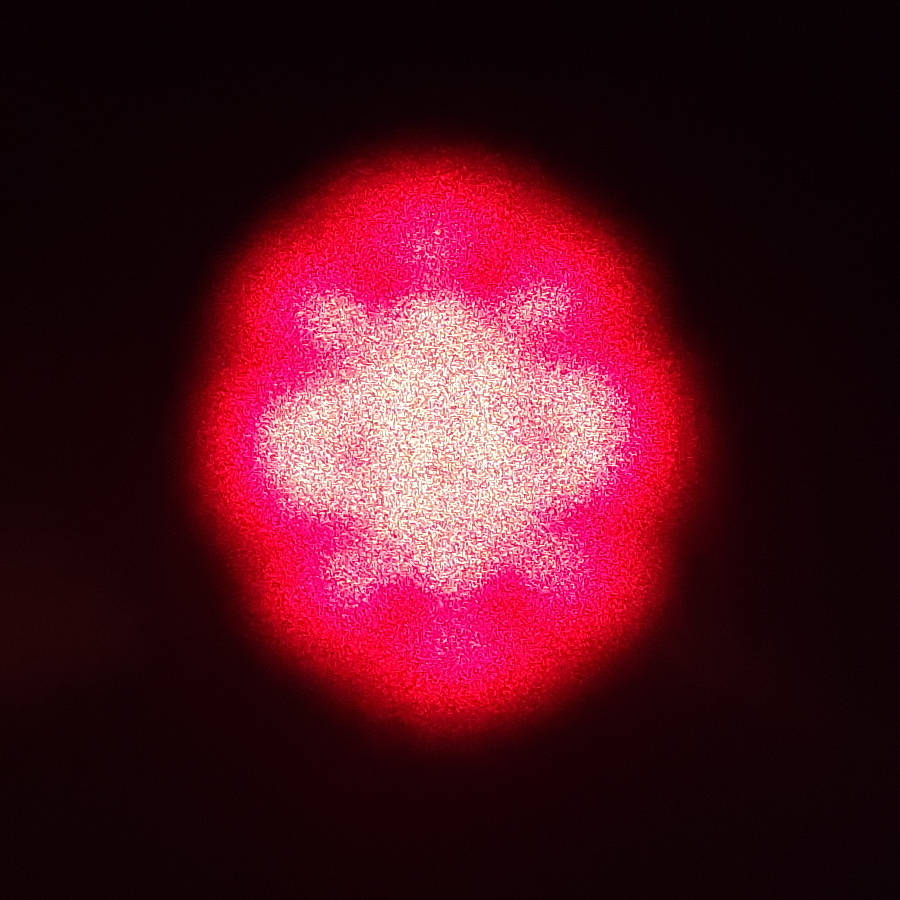
\includegraphics[width=\textwidth]{Bilder/TEM00_low.jpg}
    \caption{TEM$_{00}$, $M_y^2 = 1$}
  \end{subfigure}
  \begin{subfigure}[b!]{0.32\textwidth}
    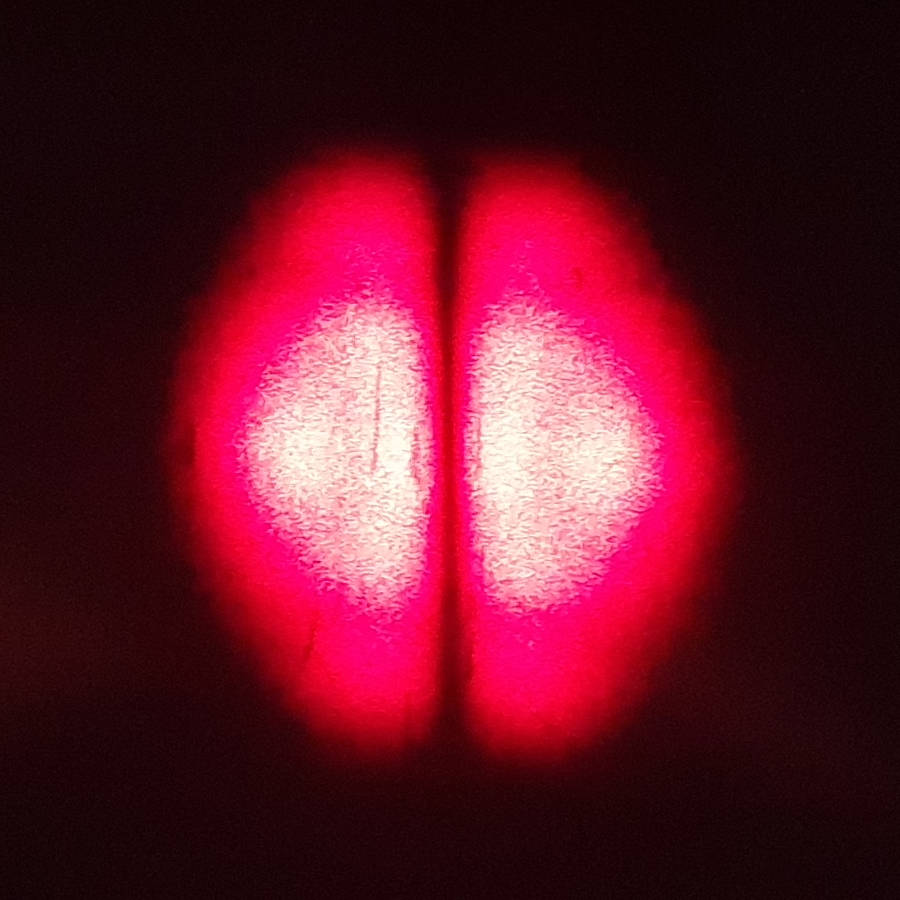
\includegraphics[width=\textwidth]{Bilder/TEM01_low.jpg}
    \caption{TEM$_{01}$, $M_y^2 = 3$}
  \end{subfigure}
  \begin{subfigure}[b!]{0.32\textwidth}
    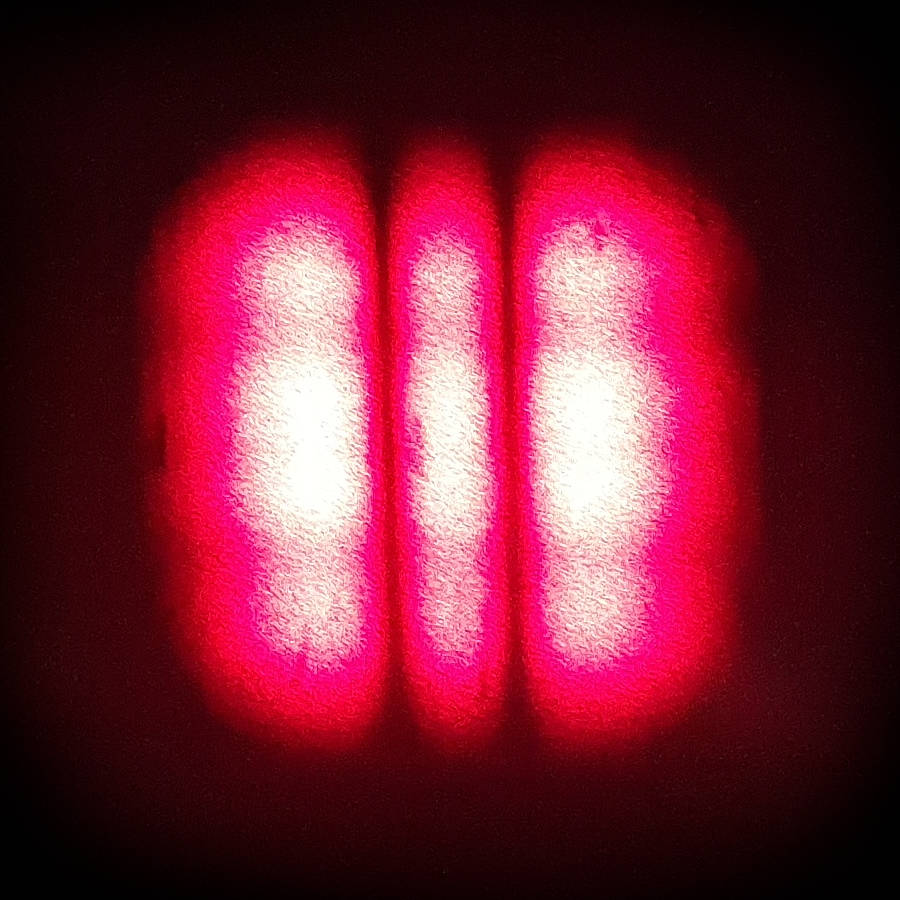
\includegraphics[width=\textwidth]{Bilder/TEM02_low.jpg}
    \caption{TEM$_{02}$, $M_y^2 = 5$}
  \end{subfigure}
  \begin{subfigure}[b!]{0.32\textwidth}
    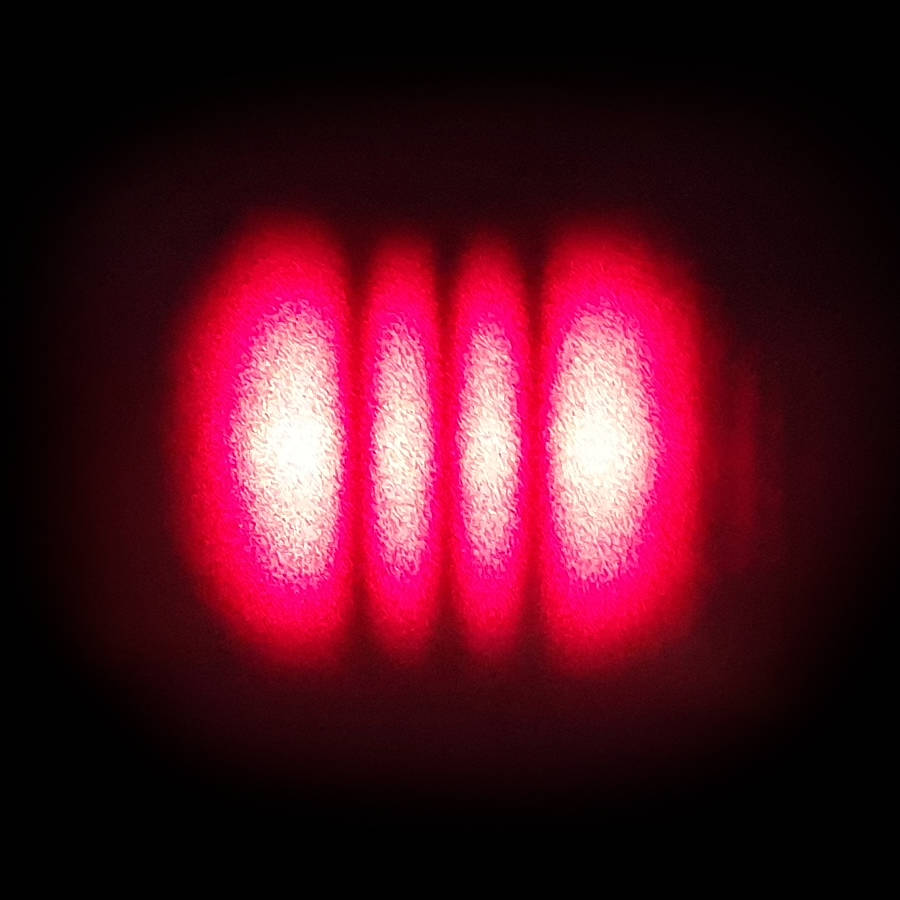
\includegraphics[width=\textwidth]{Bilder/TEM03_low.jpg}
    \caption{TEM$_{03}$, $M_y^2 = 7$}
  \end{subfigure}
  \begin{subfigure}[b!]{0.32\textwidth}
    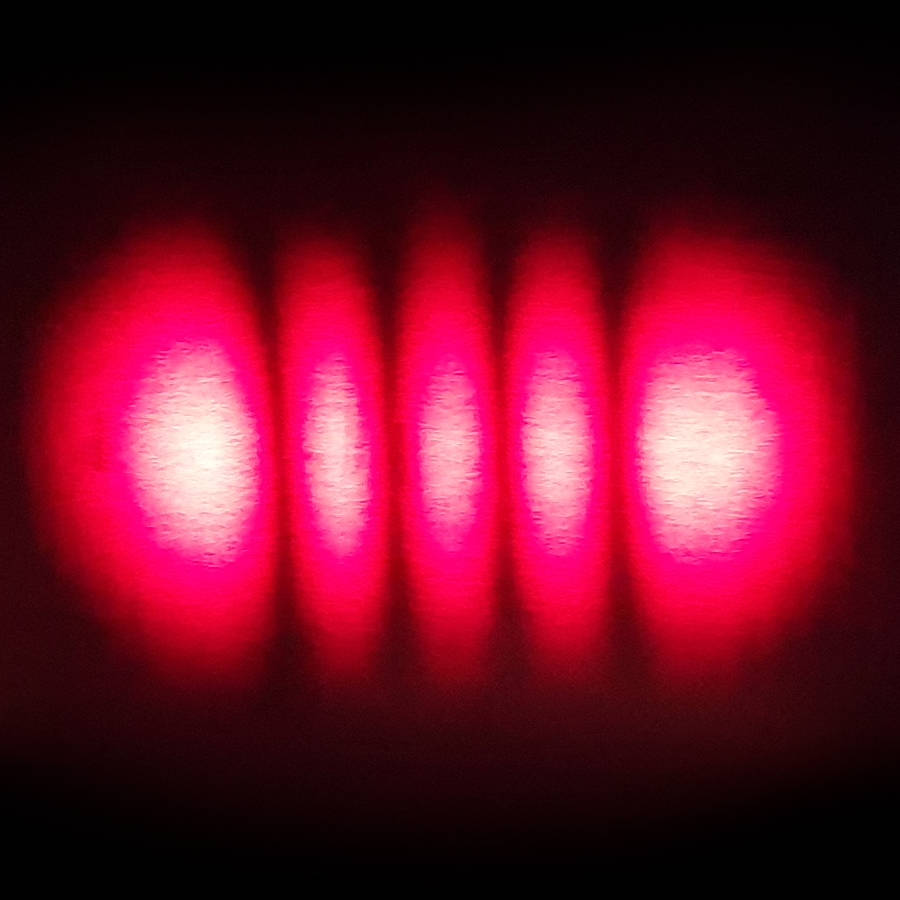
\includegraphics[width=\textwidth]{Bilder/TEM04_low.jpg}
    \caption{TEM$_{04}$, $M_y^2 = 9$}
  \end{subfigure}
  \begin{subfigure}[b!]{0.32\textwidth}
    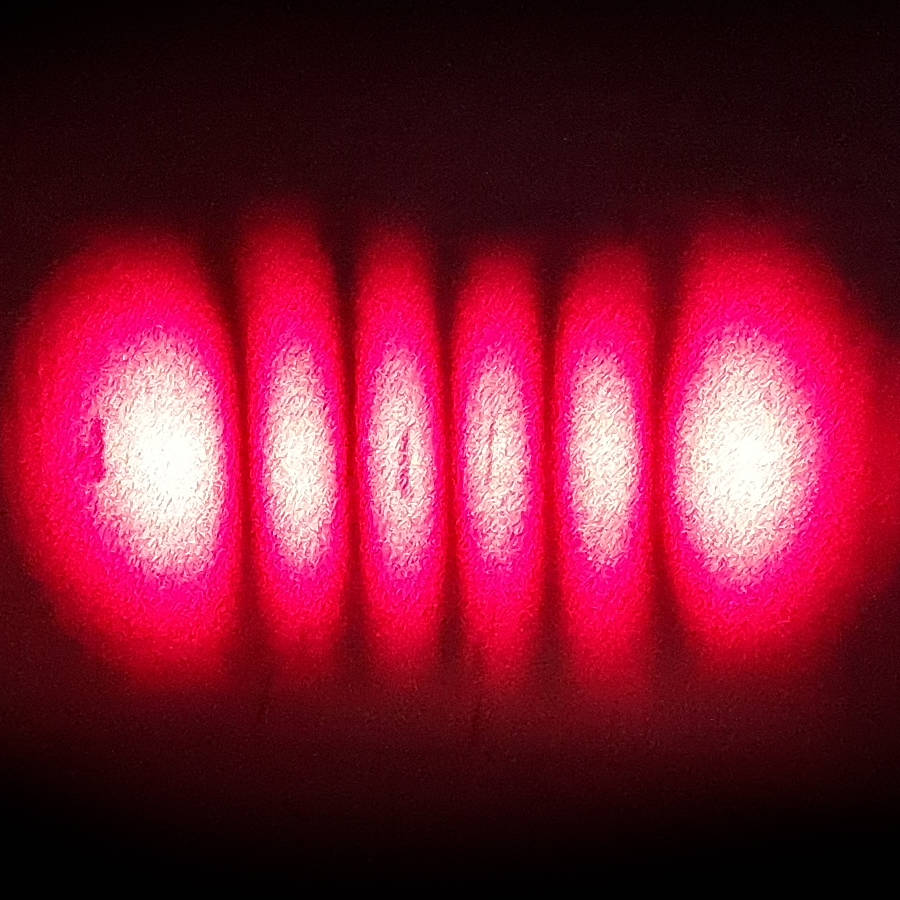
\includegraphics[width=\textwidth]{Bilder/TEM05_low.jpg}
    \caption{TEM$_{05}$, $M_y^2 = 11$}
  \end{subfigure}
  \caption{Aufgenommene Bilder verschiedener Moden bei einer Resonatorlänge von $L = \SI{0.95}{\metre}$.}
  \label{fig:TransversaleModen}
\end{figure}
\FloatBarrier

\subsection{Messungen der spektralen Intensitätsverteilung}
\subsubsection{Spektrum eines Singlemodelasers}
Um das Spektrum eines Singlemodelasers aufzunehmen wird dieser im sogenannten Wobbelungs-Betrieb betrieben. Dabei wird die Resonatorlänge $L$ des Singlemodelasers mit Hilfe einer angelegten, sich zeitlich periodisch ändernden Spannung variiert. Im Versuch wird dazu eine Dreiecksspannung verwendet. Durch diese Spannung ändert sich also die Länge des Resonators zeitlich periodisch. Da im Resonator nur stehende Wellen entstehen, muss
\begin{align}
  nL = \frac{m\lambda}{2}\quad \text{mit} \quad m \in \mathbb{N}
\end{align}

gelten. Dabei ist $n$ der Brechungsindex.
In diesem Experiment ist das zu betrachtende Medium Luft, weshalb $n=1$ gilt. Somit ergeben sich die möglichen Frequenzen bzw. Wellenlängen in Abhängigkeit der Resonatorlänge zu
\begin{align}
  \lambda = \frac{2L}{m}\quad \text{mit} \quad m \in \mathbb{N}
\end{align}
und
\begin{align}
  \nu = m \frac{c}{2L}
\end{align}
Wird also die Länge des Resonators durch das Wobbeln variiert, ändert sich die jeweilige Frequenz der Welle. \\
Im Bereich der Dreiecksspannung zwischen zwei Peaks, wo keine Vorzeichenänderung im Anstieg auftritt, ändert sich die Spannung in eine Richtung, nimmt also entweder nur zu oder nur ab. In Folge dessen ändert sich auch die Resonatorlänge in diesem Bereich nur in eine Richtung. Hierbei wird ein charakteristischer Verlauf der Intensität beobachtet, der in Abbildung \ref{fig:Zeitverlauf} dargestellt ist.

\begin{figure}[htp]
    \centering
        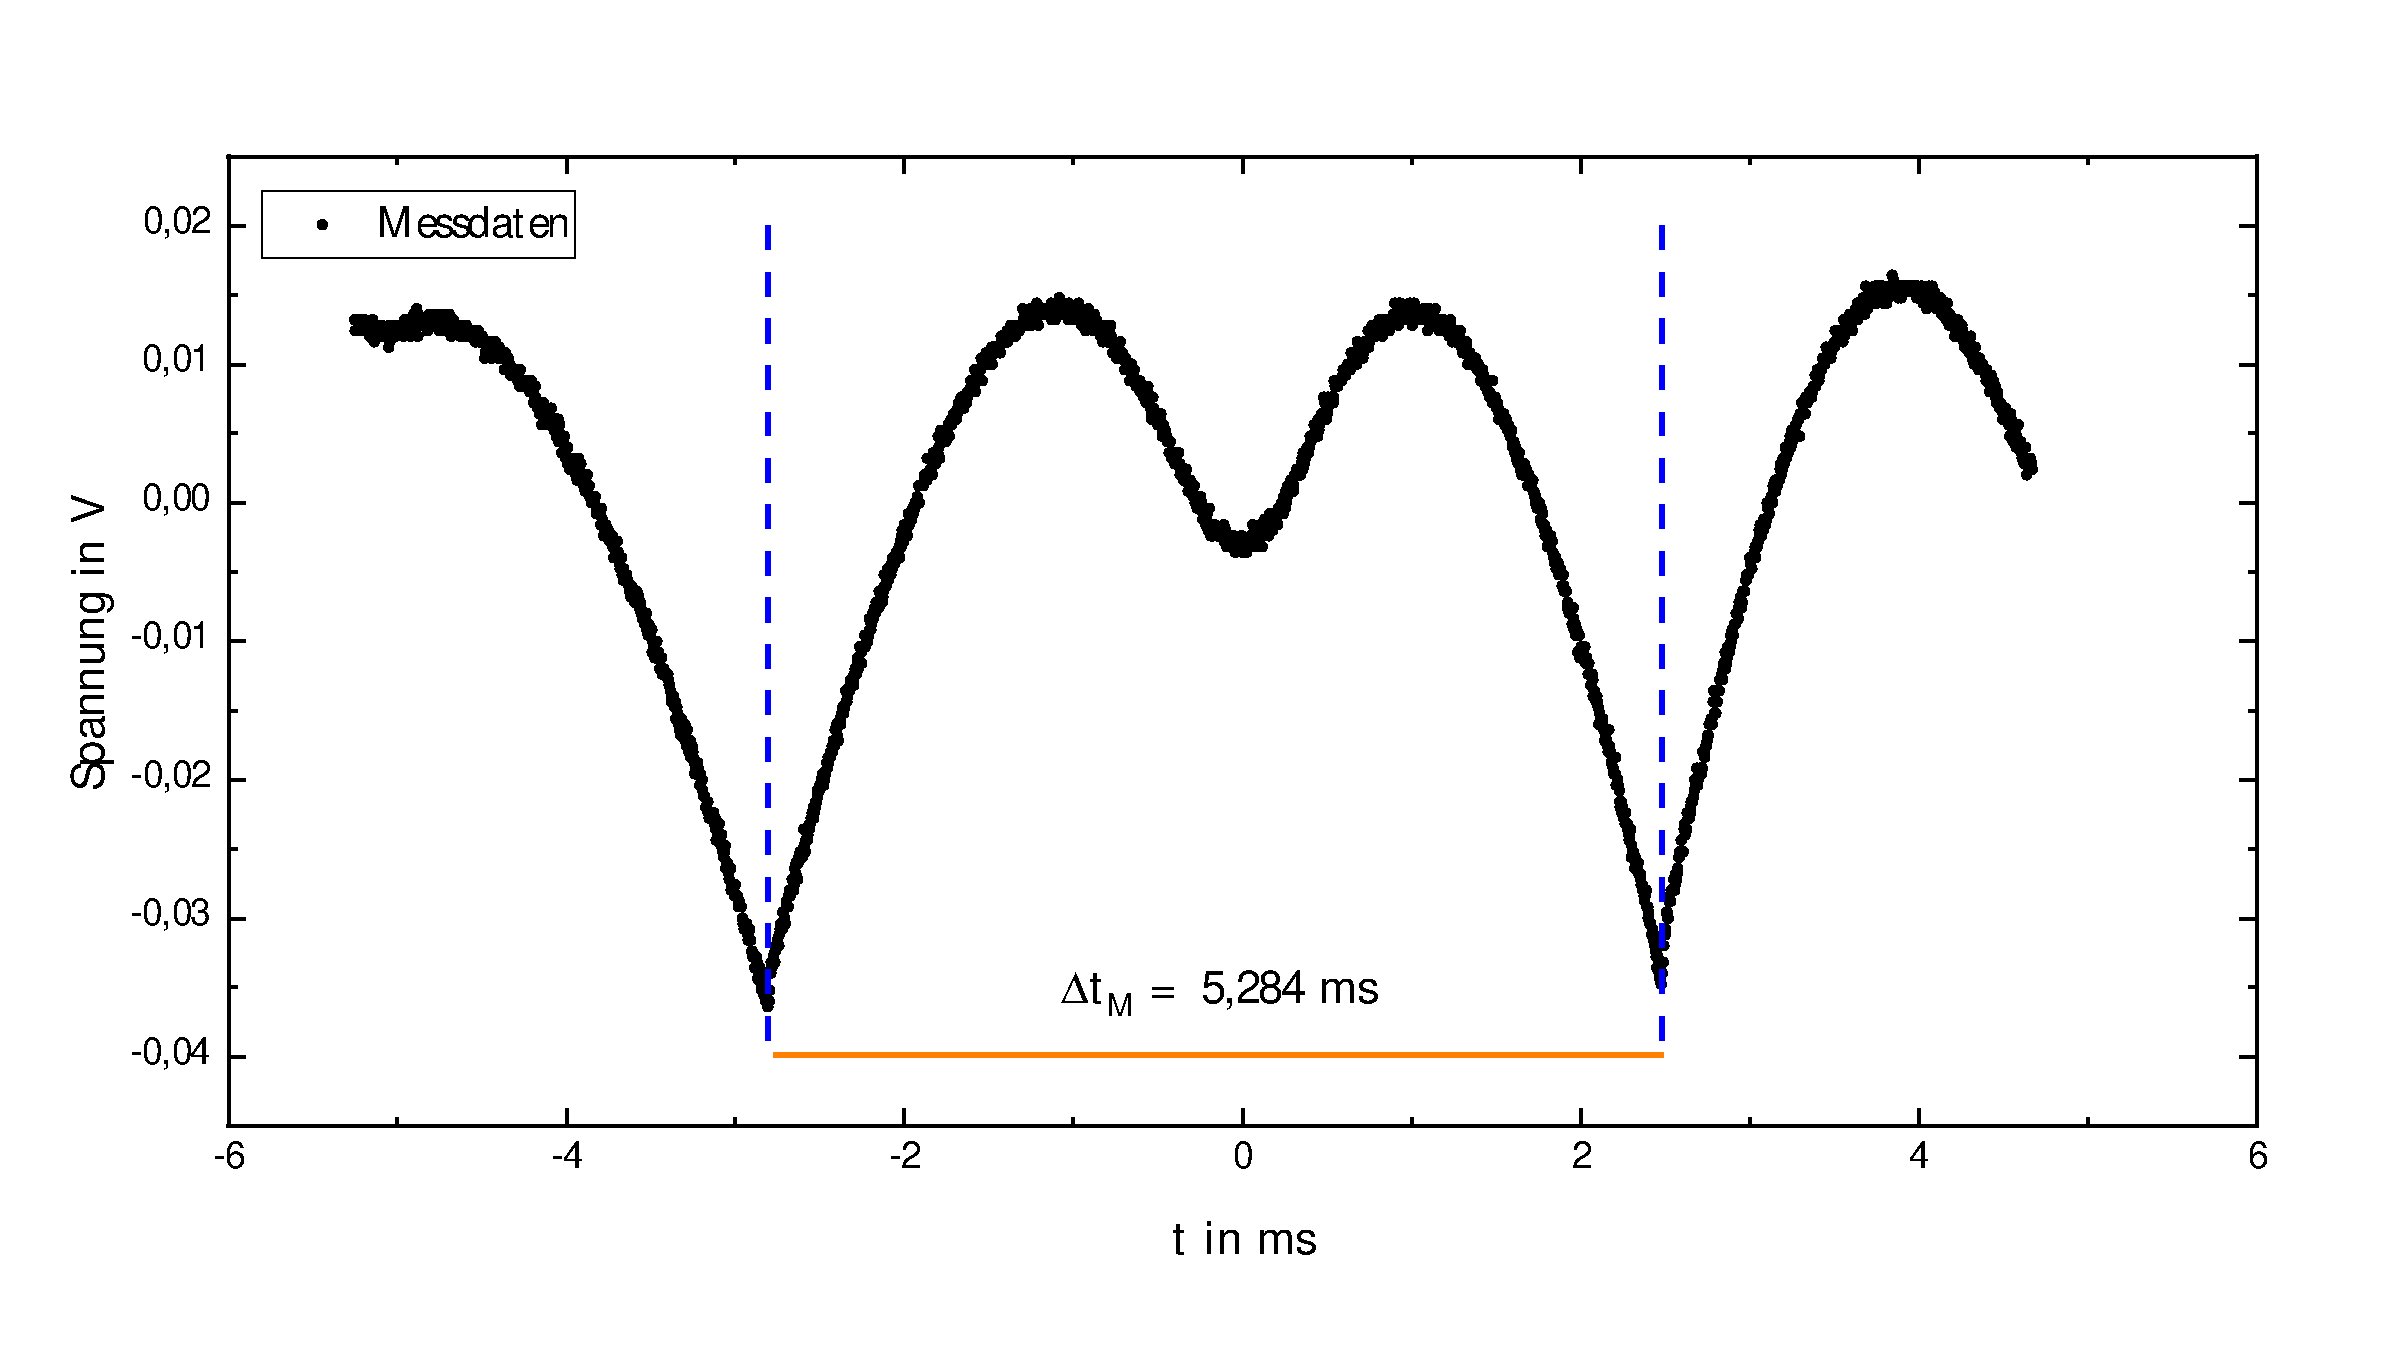
\includegraphics[width=1\textwidth]{Bilder/Profil_SML_Zeitverlauf.pdf}
    \caption{Zeitverlauf der Intensität des Singlemodelasers bei Wobbelung mit Dreiecksspannung.}
    \label{fig:Zeitverlauf}
\end{figure}

Jener stellt sich als ein sich periodisch wiederholenden Gauß dar, welcher eine Eindellung in der Mitte aufweist. Dies ergibt sich, da die Modenfrequenz sich bei in eine Richtung ändernde Resonatorlänge so verändert, dass sie sich unter dem aus der Linienbreite gegebenen Verstärkungsprofil \glqq in einer Richtung (abhängig davon ob ansteigende oder abfallende Spannung und damit vergrößernder oder verkleinernder Resonator) hindurchbewegt\grqq. Abhängig von der Frequenz, die sich in Folge der sich über die Zeit ändernden Dreiecksspannung auch periodisch ändert, tritt unterschiedlich starke Verstärkung auf. Entscheidend ist hier, dass sich der Verlauf bei weiter in eine Richtung ändernde Dreiecksspannung, also z.\,B. weiter vergrößern der Resonatorlänge, wiederholt. Das liegt daran, dass dann die zweite Mode, die sich im charakteristischen Abstand
\begin{align}
  \Delta \nu = \frac{c}{2nL}
\end{align}
befindet, sich, bildlich gesprochen, unter das Verstärkungsprofil schiebt. Aus dieser Überlegung ergibt sich, dass der Abstand der Nullstellen, wo sich also der charakteristische Verlauf der Kurve zu wiederholen beginnt, der Abstand zweier Moden entspricht.\\
Diese Überlegung erlaubt es, eine Umrechnung von Zeitbereich in Frequenzbereich durchzuführen. Es gilt
\begin{align}
  \Delta \nu = \Delta \text{t}
\end{align}.
und
\begin{align}
  \Delta \nu = \frac{c}{2nL} \overset{n=1}{=} \frac{c}{2L} \overset{L=\SI{0,17}{\meter}}{=} \frac{c}{2\cdot \SI{0,17}{\meter}}=\SI{881}{\mega\hertz}
\end{align}
sowie
\begin{align}
  \Delta \text{t} \overset{s. Abb.}=\SI{5,28}{\milli\second}
\end{align}
und damit
\begin{align}
  \SI{1}{\milli\second}=\SI{1,67}{\mega\hertz}
\end{align}

Diese Umrechnung ermöglicht eine Darstellung im Frequenzbereich, der in Abbildung \ref{fig:Frequenzverlauf} dargestellt ist.

\begin{figure}[htp]
    \centering
        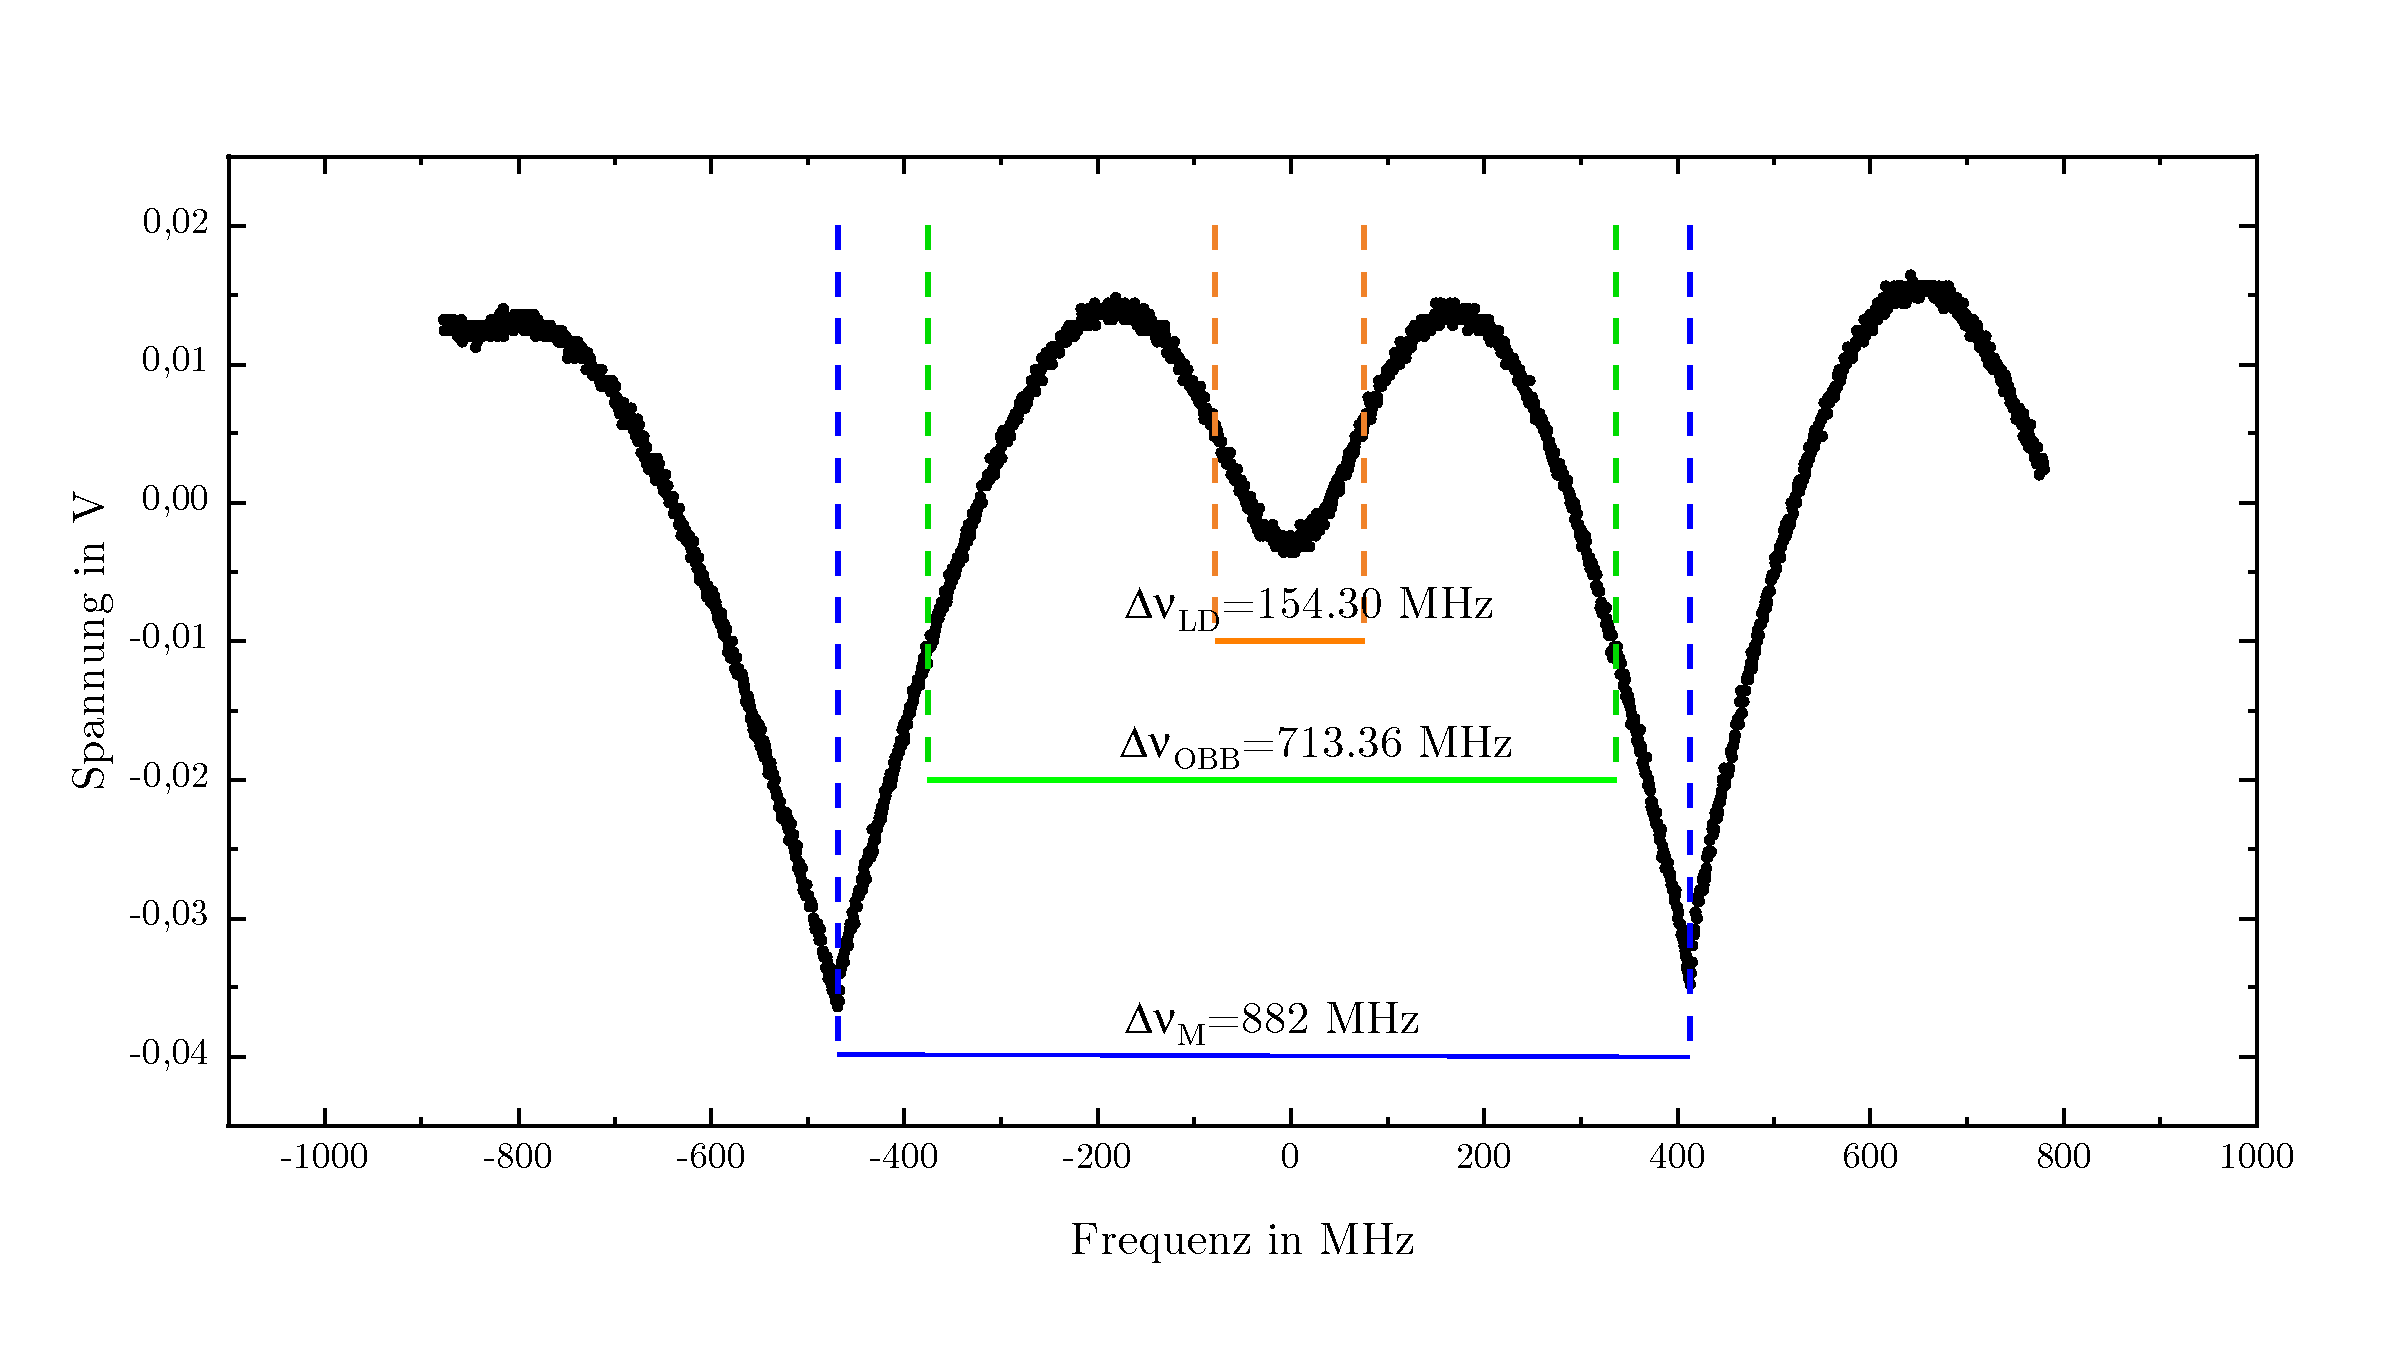
\includegraphics[width=1\textwidth]{Bilder/Profil_SML_Frequenzbild.pdf}
    \caption{Frequenzspektrum des Singlemodelasers}
    \label{fig:Frequenzverlauf}
\end{figure}

Hieran kann nun die \textit{Oszillationsbandbreite} des Singlemodelasers als Halbwertsbreite des Spektrums auf
\begin{align}
  \Delta \nu = \SI{713}{\mega\hertz}
\end{align}
bestimmt werden.\\
Das theoretische \textit{Auflösungsvermögen} dieses Spektrometers ist bestimmt durch die Diskretisierung des Oszilloskops, ergibt sich aus dem Abstand der Samplepunkte dieses und beläuft sich auf \SI{0,7}{\mega\hertz}. Bei einem Wellenlängenbereich von \SI{632,8}{\nano\meter}, was einer Frequenz von \SI{474}{\tera\hertz} entspricht,  ergibt sich ein spektrales Auflösungsvermögen von
\begin{align}
  \frac{\nu}{\Delta\nu} \approx 6,8\cdot10^8
\end{align}
Im \textit{Vergleich zum Auflösungsvermögen eines Prismas} wird deutlich, welche entscheidende Verbesserung durch das Laserspektrometer gewonnen werden kann. Bei einem Flintglas-Prisma mit der Basislänge $b =\SI{1}{\centi\meter}$ beläuft sich die Auflösung auf $A \approx 10^3$, was um vielen Größenordnungen unter der Auflösung des Laserspektrometers liegt. \\
An der Darstellung des Frequenzspektrums in Abbildung \ref{fig:Frequenzverlauf} ist deutlich die Eindellung in der Mitte des Spektrums, der sogenannte \textit{Lamb-Dip} zu sehen. Der dieser Eindellung zugrunde liegende Effekt ist, wie in Abschnitt \ref{sec:InversionsabbauLambDip} beschrieben, der Dopplereffekt. Ebenso ist dort begründet, dass die Breite des Lamb-Dips ungefähr der homogenen Linienverbreiterung entspricht, sodass wir mit den Daten aus Abbildung \ref{fig:Frequenzverlauf} für die homogene Linienverbreiterung erhalten
\begin{align}
  \Delta \nu_{HL} \approx \SI{154,3}{\mega \hertz}
\end{align}
Die Dopplerbreite liegt dagegen bei
\begin{align}
  \Delta \nu_{D}= \frac{f_0}{c} \sqrt{\frac{8 k_B T \text{ln} 2}{\text{m}}} = \SI{1,5}{\giga\hertz} \qquad \text{mit}\quad \text{m} = \text{m}_{\text{Ne}}
 = \SI{20,1797}{u} \qquad \text{und} \quad T= \SI{400}{K}
\end{align}
und die natürliche Linienbreite bei
\begin{align}
  \Delta \nu = \frac{1}{2\pi\tau}\approx \SI{16}{\mega\hertz}
\end{align}
Somit wird deutlich, dass die Dopplerverbreiterung die entscheidende Verbreiterung bei diesem Übergang ist.

\subsubsection{optisches Heterodyn}
Indem der Singlemodelaser im Wobbelungsbetrieb mit dem Multimodelaser überlagert wird, lassen sich die Lagen der Axialmoden des Multimodelasers feststellen: Immer dann, wenn die Frequenz des Singlemodelasers, die durch die Wobbelung periodisch variiert wird, mit der Frequenz des Multimodelasers übereinstimmt, kommt es zur konstruktiven Interferenz und auf dem Spektrum tritt ein Ausschlag auf. \\
Zu beachten ist, dass damit die Interferenz überhaupt mit dem integrierenden Photodetektor detektiert werden kann, die Abstände der Interferenzmaxima kleiner seien müssen als die Ausdehnung des Photodetektors. Mit einfachen geometrischen Überlegungen ergibt sich, dass bei einer Detektorausdehnung von \SI{1}{\milli\meter} der Winkel der beiden Laser sich nur um $6\cdot 10^{-4}$ unterscheiden darf. Es ist also eine sehr genaue Justage und ein möglichst großer Abstand zwischen Detektor und Lasern nötig. \\
Der Aufbau hat sich dahingehend verändert, dass eine Irisblende in den Strahlengang eingesetzt wurde. Durch diese werden höhere Transversalmoden geblockt, denn diese haben ihre Intensität hauptsächlich in größerem radialen Abstand. Durch die teilweise geschlossene Irisblende werden die Verluste für diese Transversalmoden als so erhöht, dass diese nach der zweiten Laserbedingung nicht mehr anschwingen können. \\
Es werden mehrere Schwerpunkte untersucht. Zum einen werden die Resonatorenlängen variiert, um zu untersuchen bzw. darzustellen, dass sich, wie die Theorie es vorhersagt, bei längerer Resonatorlänge, mehrere Axialmoden ausbilden. Dies ist in Abbildung \ref{fig:Resonatorveränderung} zu sehen. Hierbei wurden durch eine Irisblende wie oben beschrieben alle Transversalmoden verhindert, weshalb sich in den Messungen nur eine Transversalmode, die Grundmode, ausgebildet hat.

\begin{figure}[htp]
  \centering
  \begin{subfigure}{0.8\textwidth}
    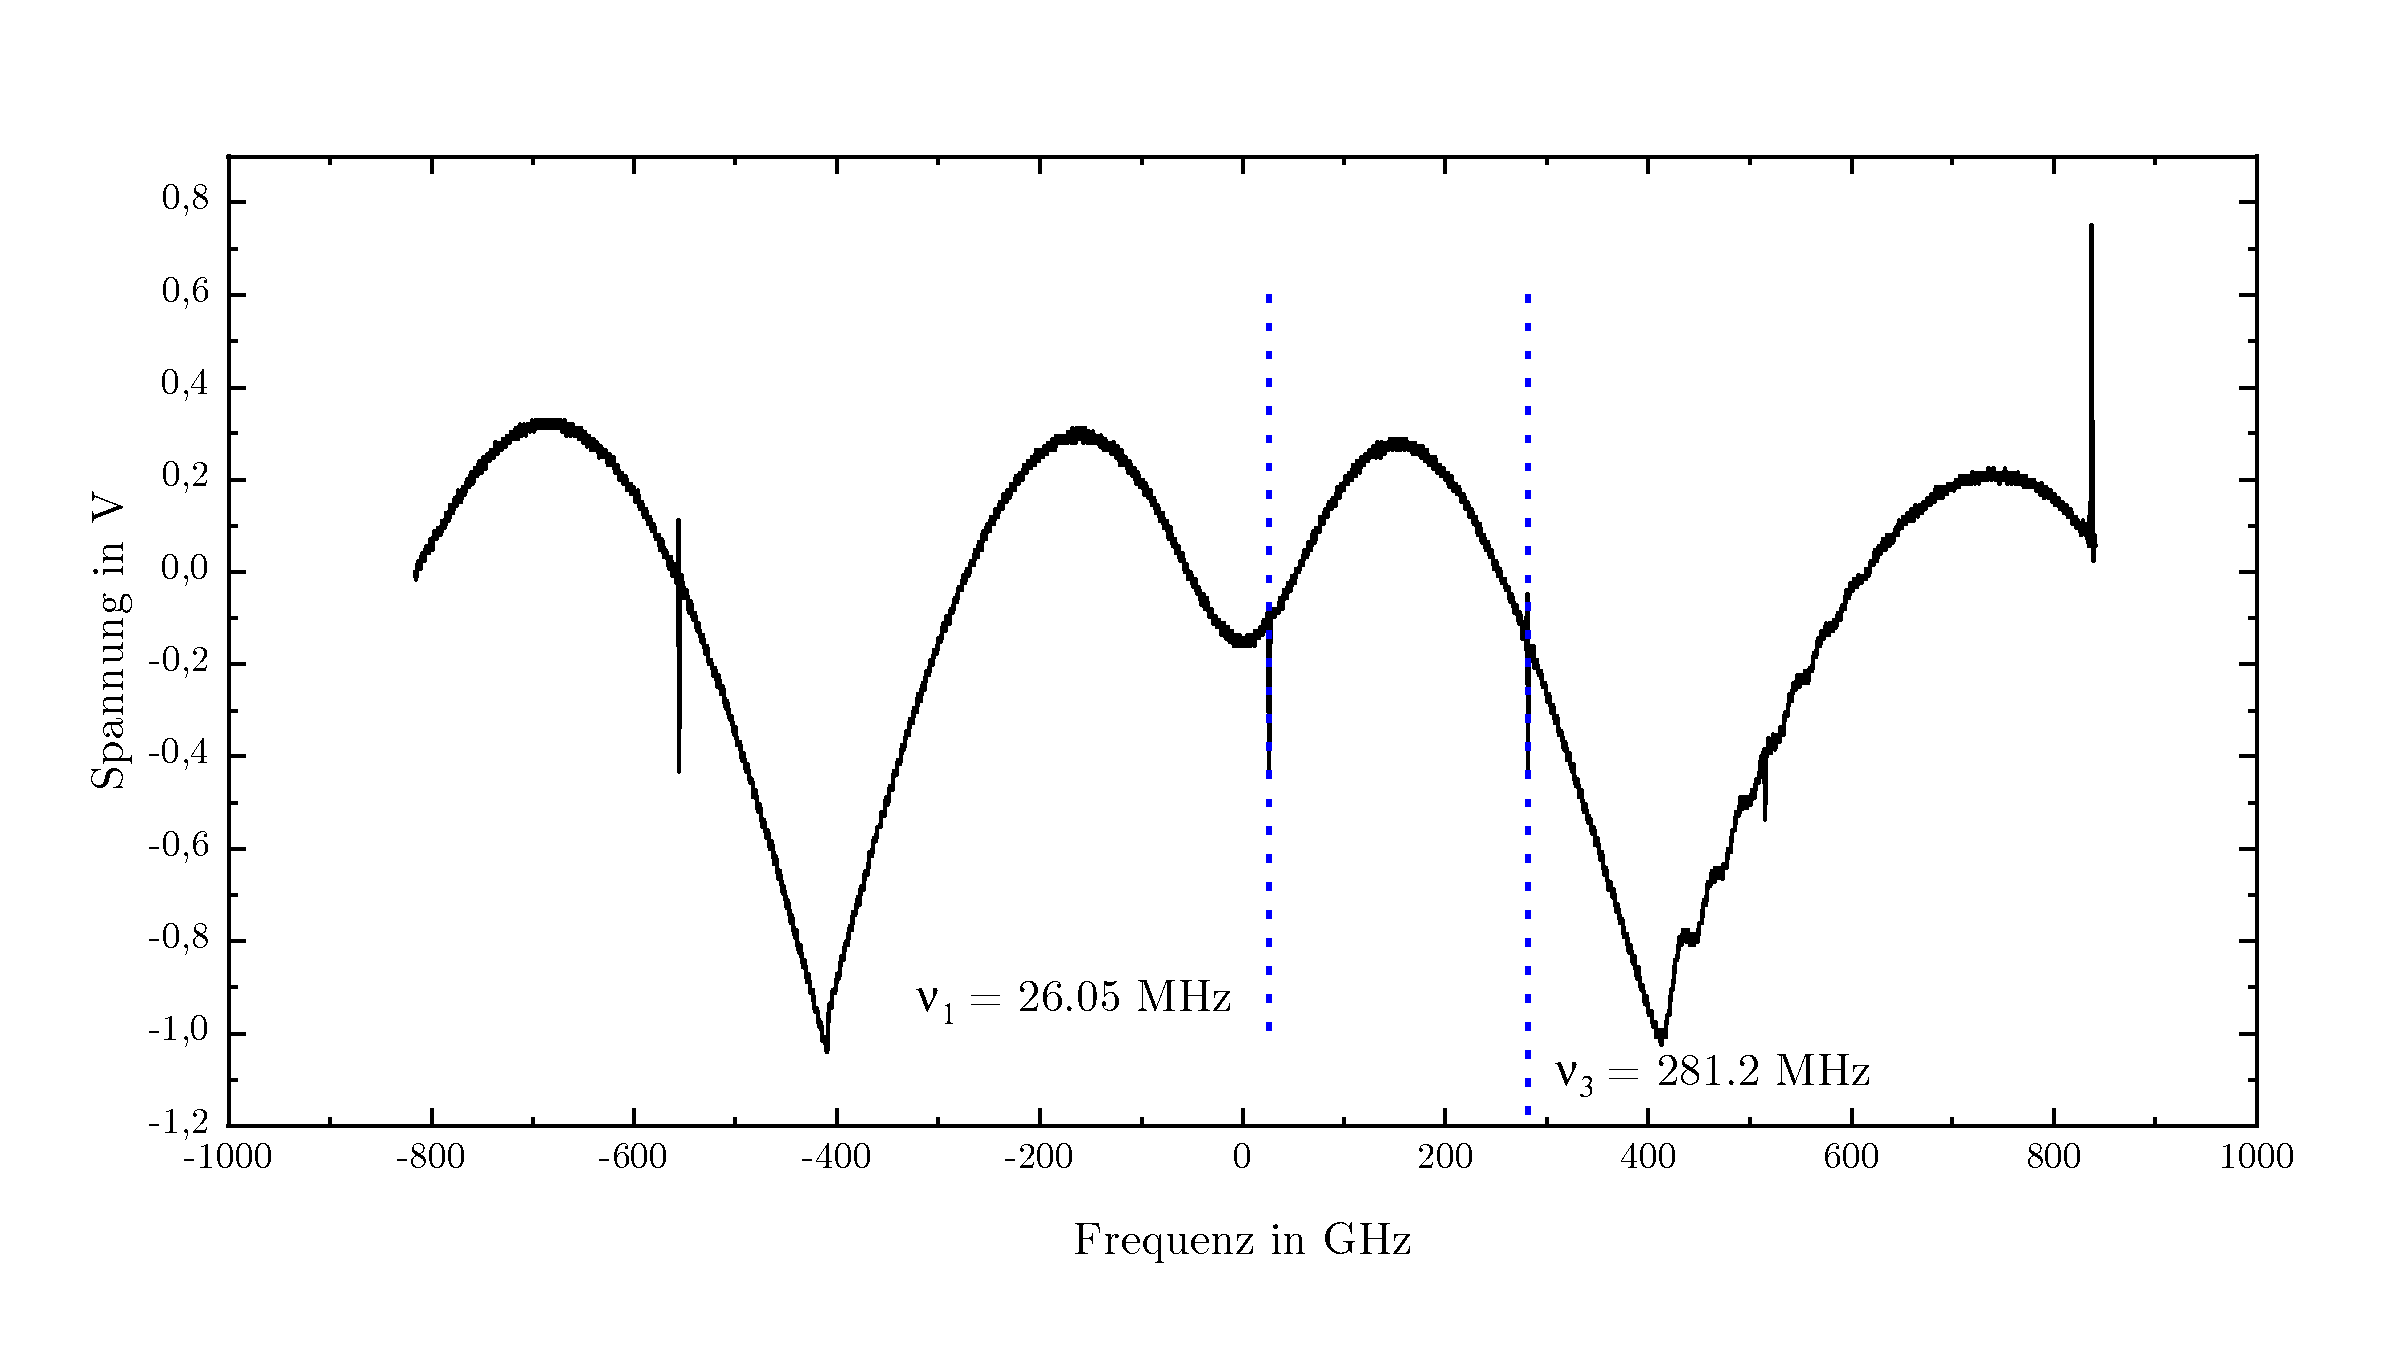
\includegraphics[width=\textwidth]{Bilder/mehrereResonatorlaengen_50cm_1Mode.pdf}
    \caption{Resonatorlänge \SI{50}{\centi\meter}}
  \end{subfigure}
  \begin{subfigure}{0.8\textwidth}
    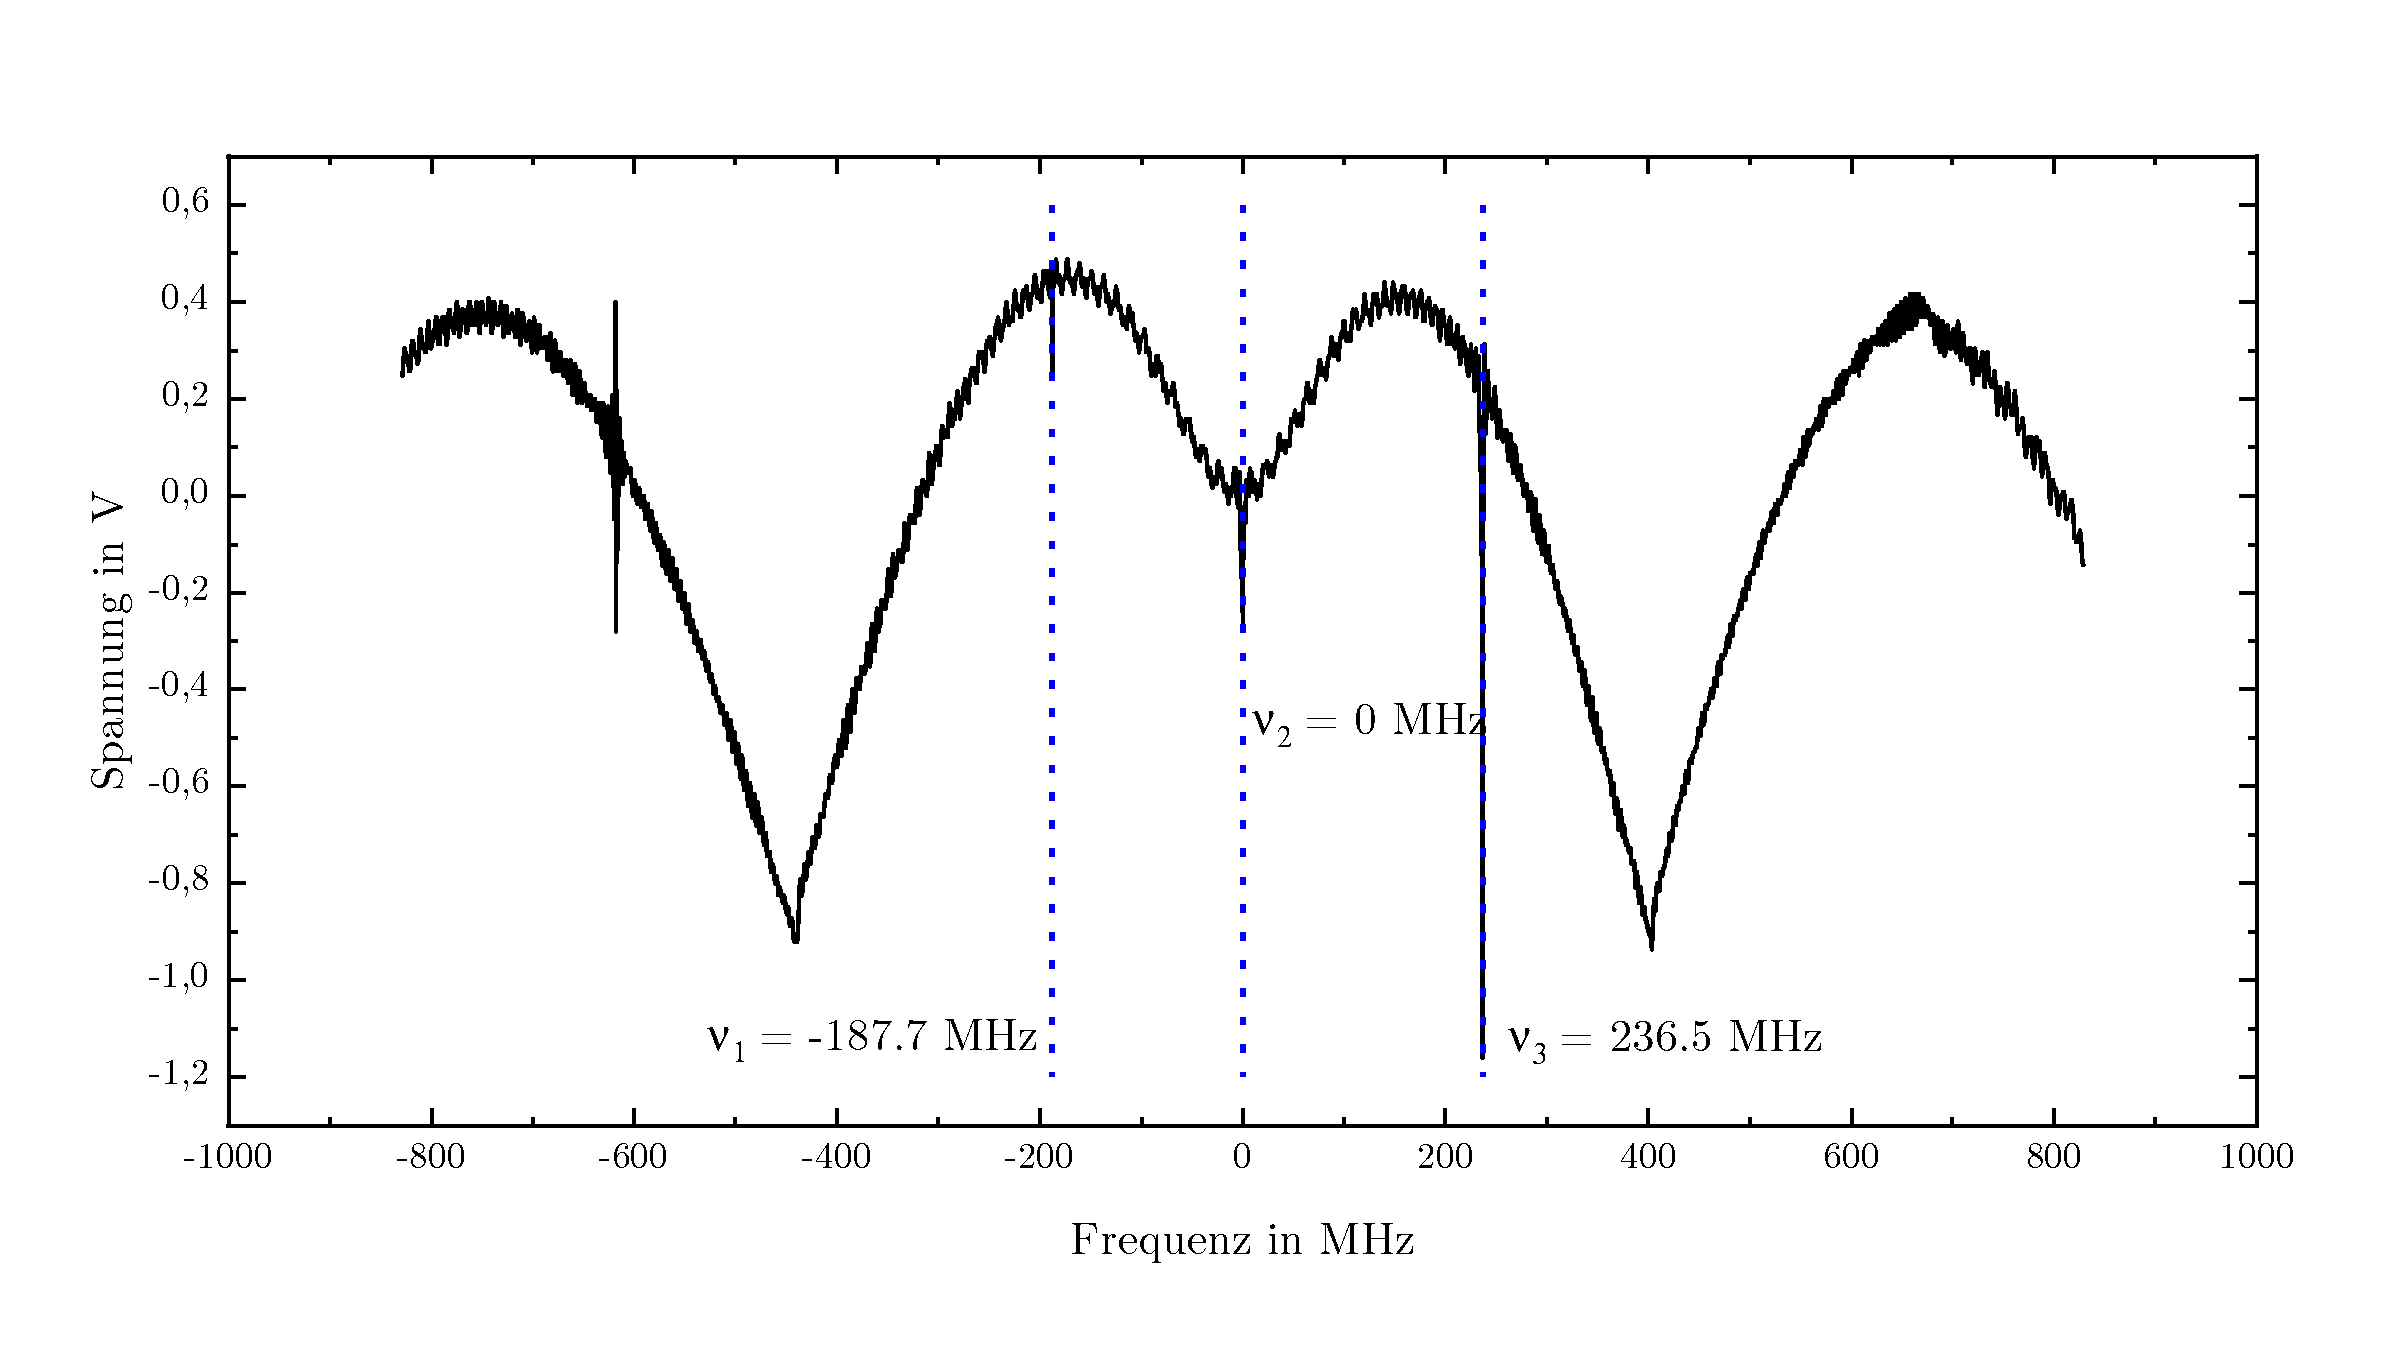
\includegraphics[width=\textwidth]{Bilder/mehrereResonatorlaengen_75cm_1Mode.pdf}
    \caption{Resonatorlänge \SI{75}{\centi\meter}}
  \end{subfigure}
  \begin{subfigure}{0.8\textwidth}
    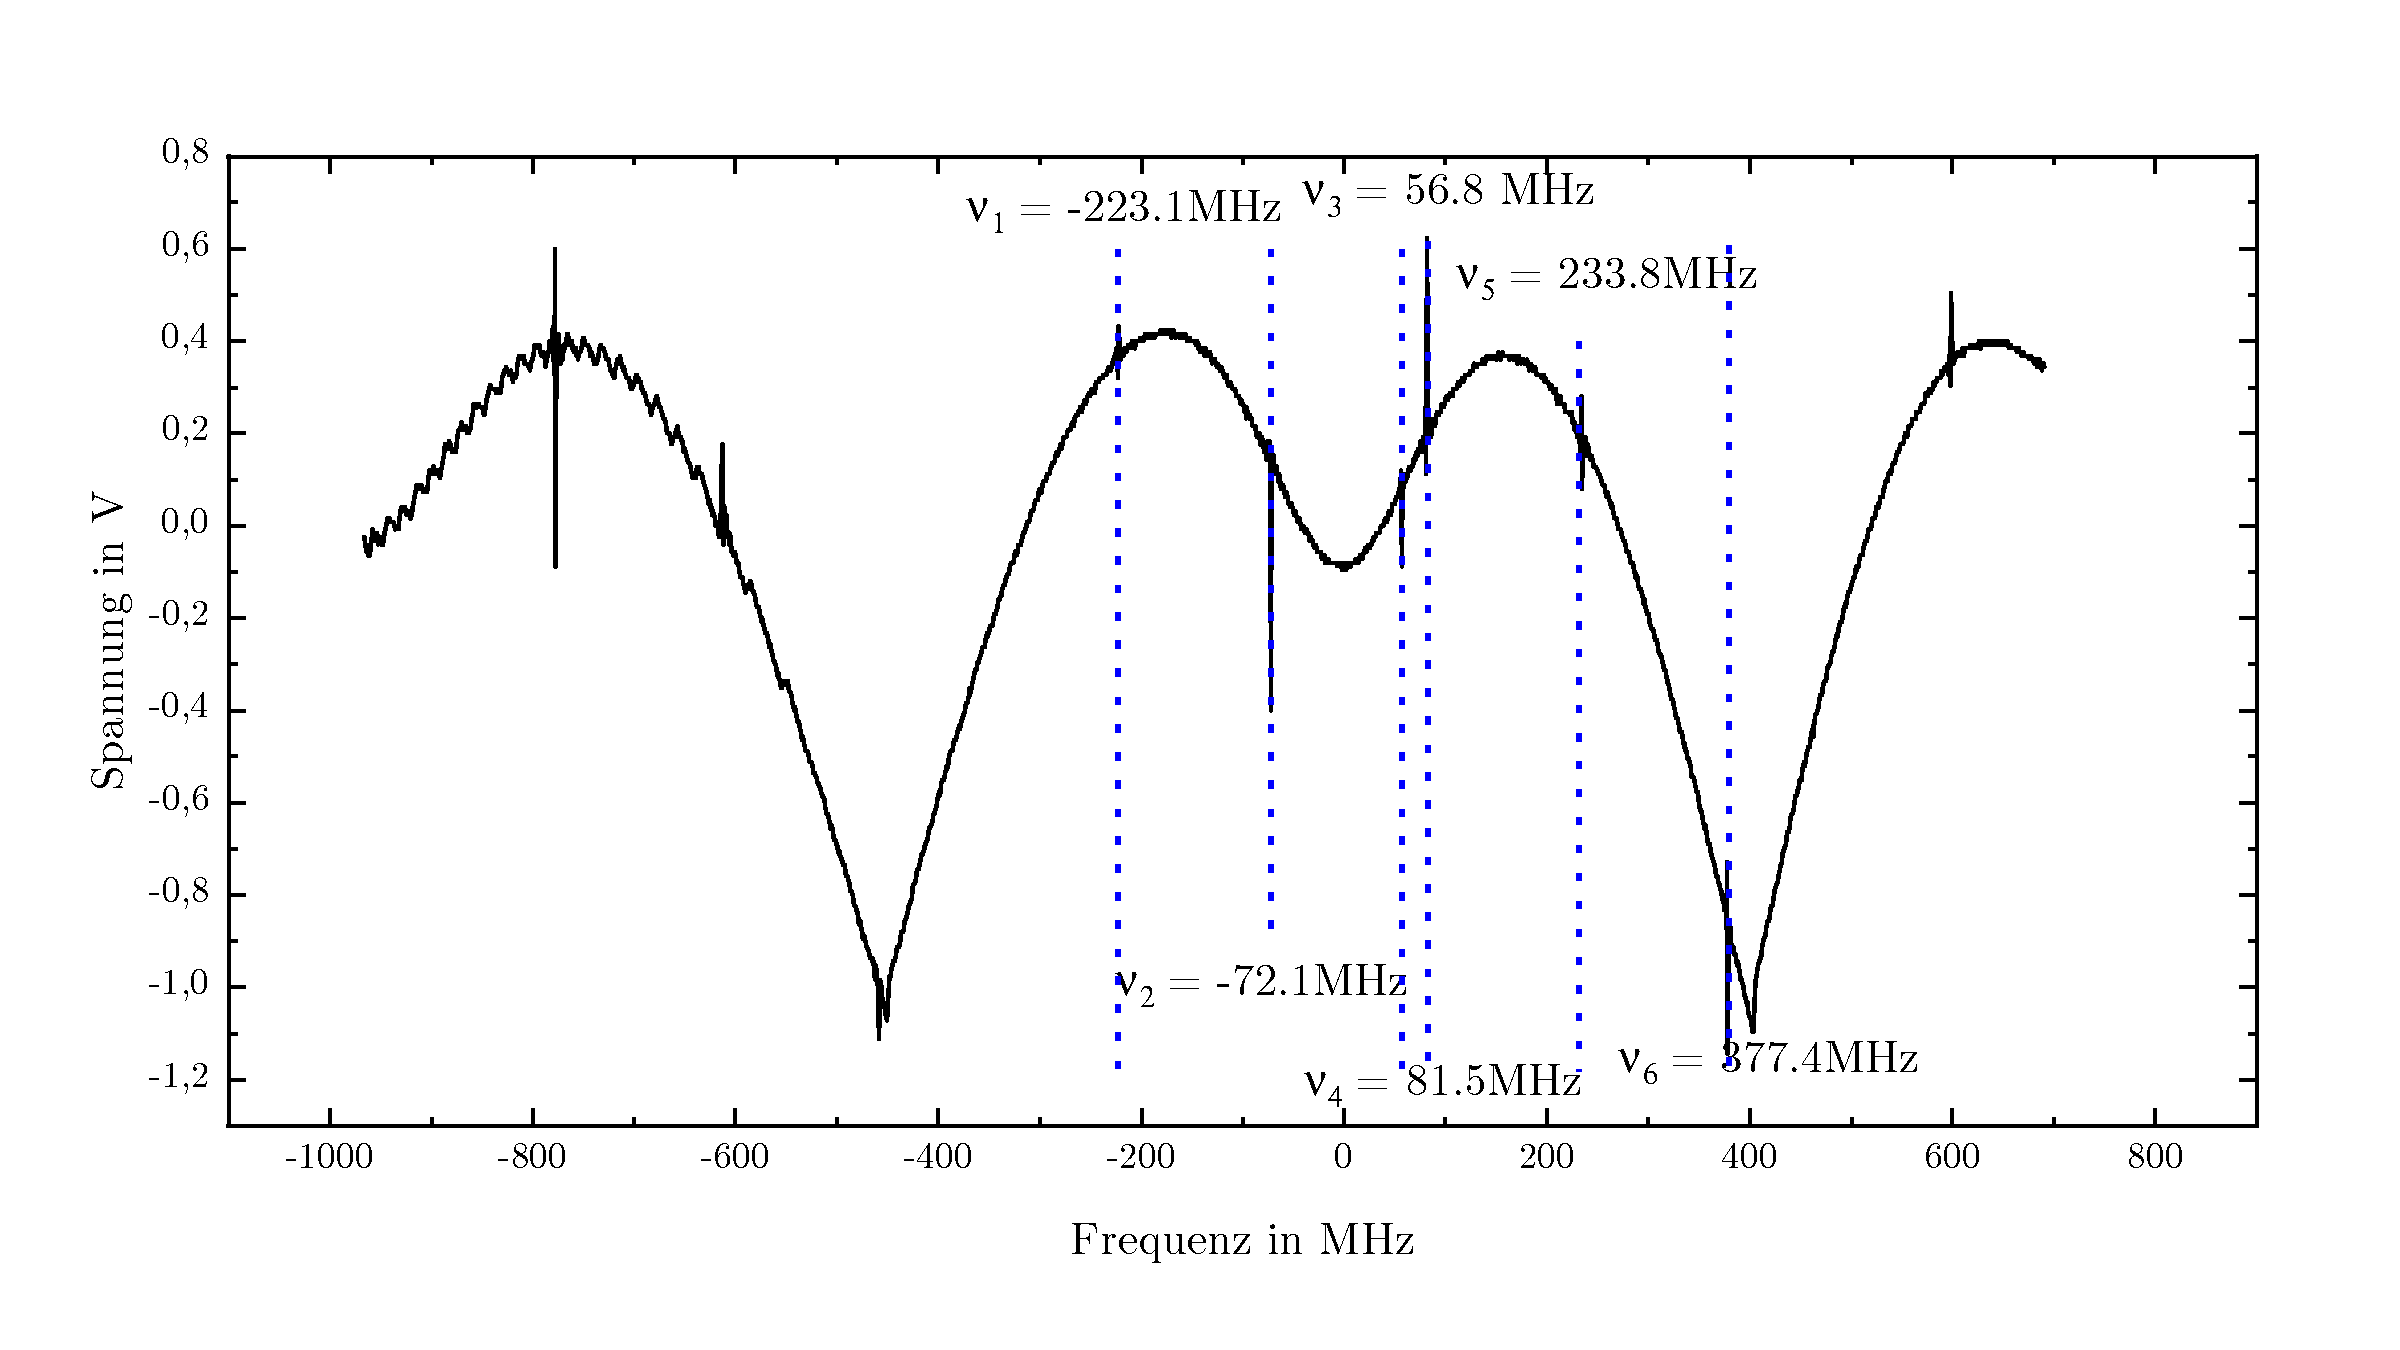
\includegraphics[width=\textwidth]{Bilder/1TransversaleMode_94cm.pdf}
    \caption{Resonatorlänge \SI{94}{\centi\meter}}
  \end{subfigure}
  \caption{Signal des SML überlagert mit MML bei unterschiedlichen Resonatorlängen des MML. Höhere Transversalmoden durch Irisblende geblockt. Nur Grundmode kann anschwingen}
  \label{fig:Resonatorveränderung}
\end{figure}

\FloatBarrier

Der oben theoretisch hergeleitete Einfluss der Irisblende wird in folgender Messung, die in Abbildung \ref{fig:Transversalemode} dargestellt ist, nachgewiesen. Während der ersten Messung war die Irisblende soweit geschlossen, dass bereits die erste höhere Transversalmode ausgeblendet war. In der zweiten Messung wurde sie soweit geöffnet, dass erst die dritte Transversalmode die Blende nicht passieren konnte. Dass in Messung zwei die zweite Transversalmode tatsächlich anschwingt, wird an den nur in kleinem Abstand zur ersten Mode auftretenden Intensitätsverstärkung deutlich. Jeweils gleiche Frequenzen, also die der jeweils zweiten Transversalmoden haben wieder den gleichen Abstand. Es wurde eine Resonatorlänge von \SI{94}{\centi\meter} verwendet.

\begin{figure}[htp]
  \centering
  \begin{subfigure}{0.8\textwidth}
    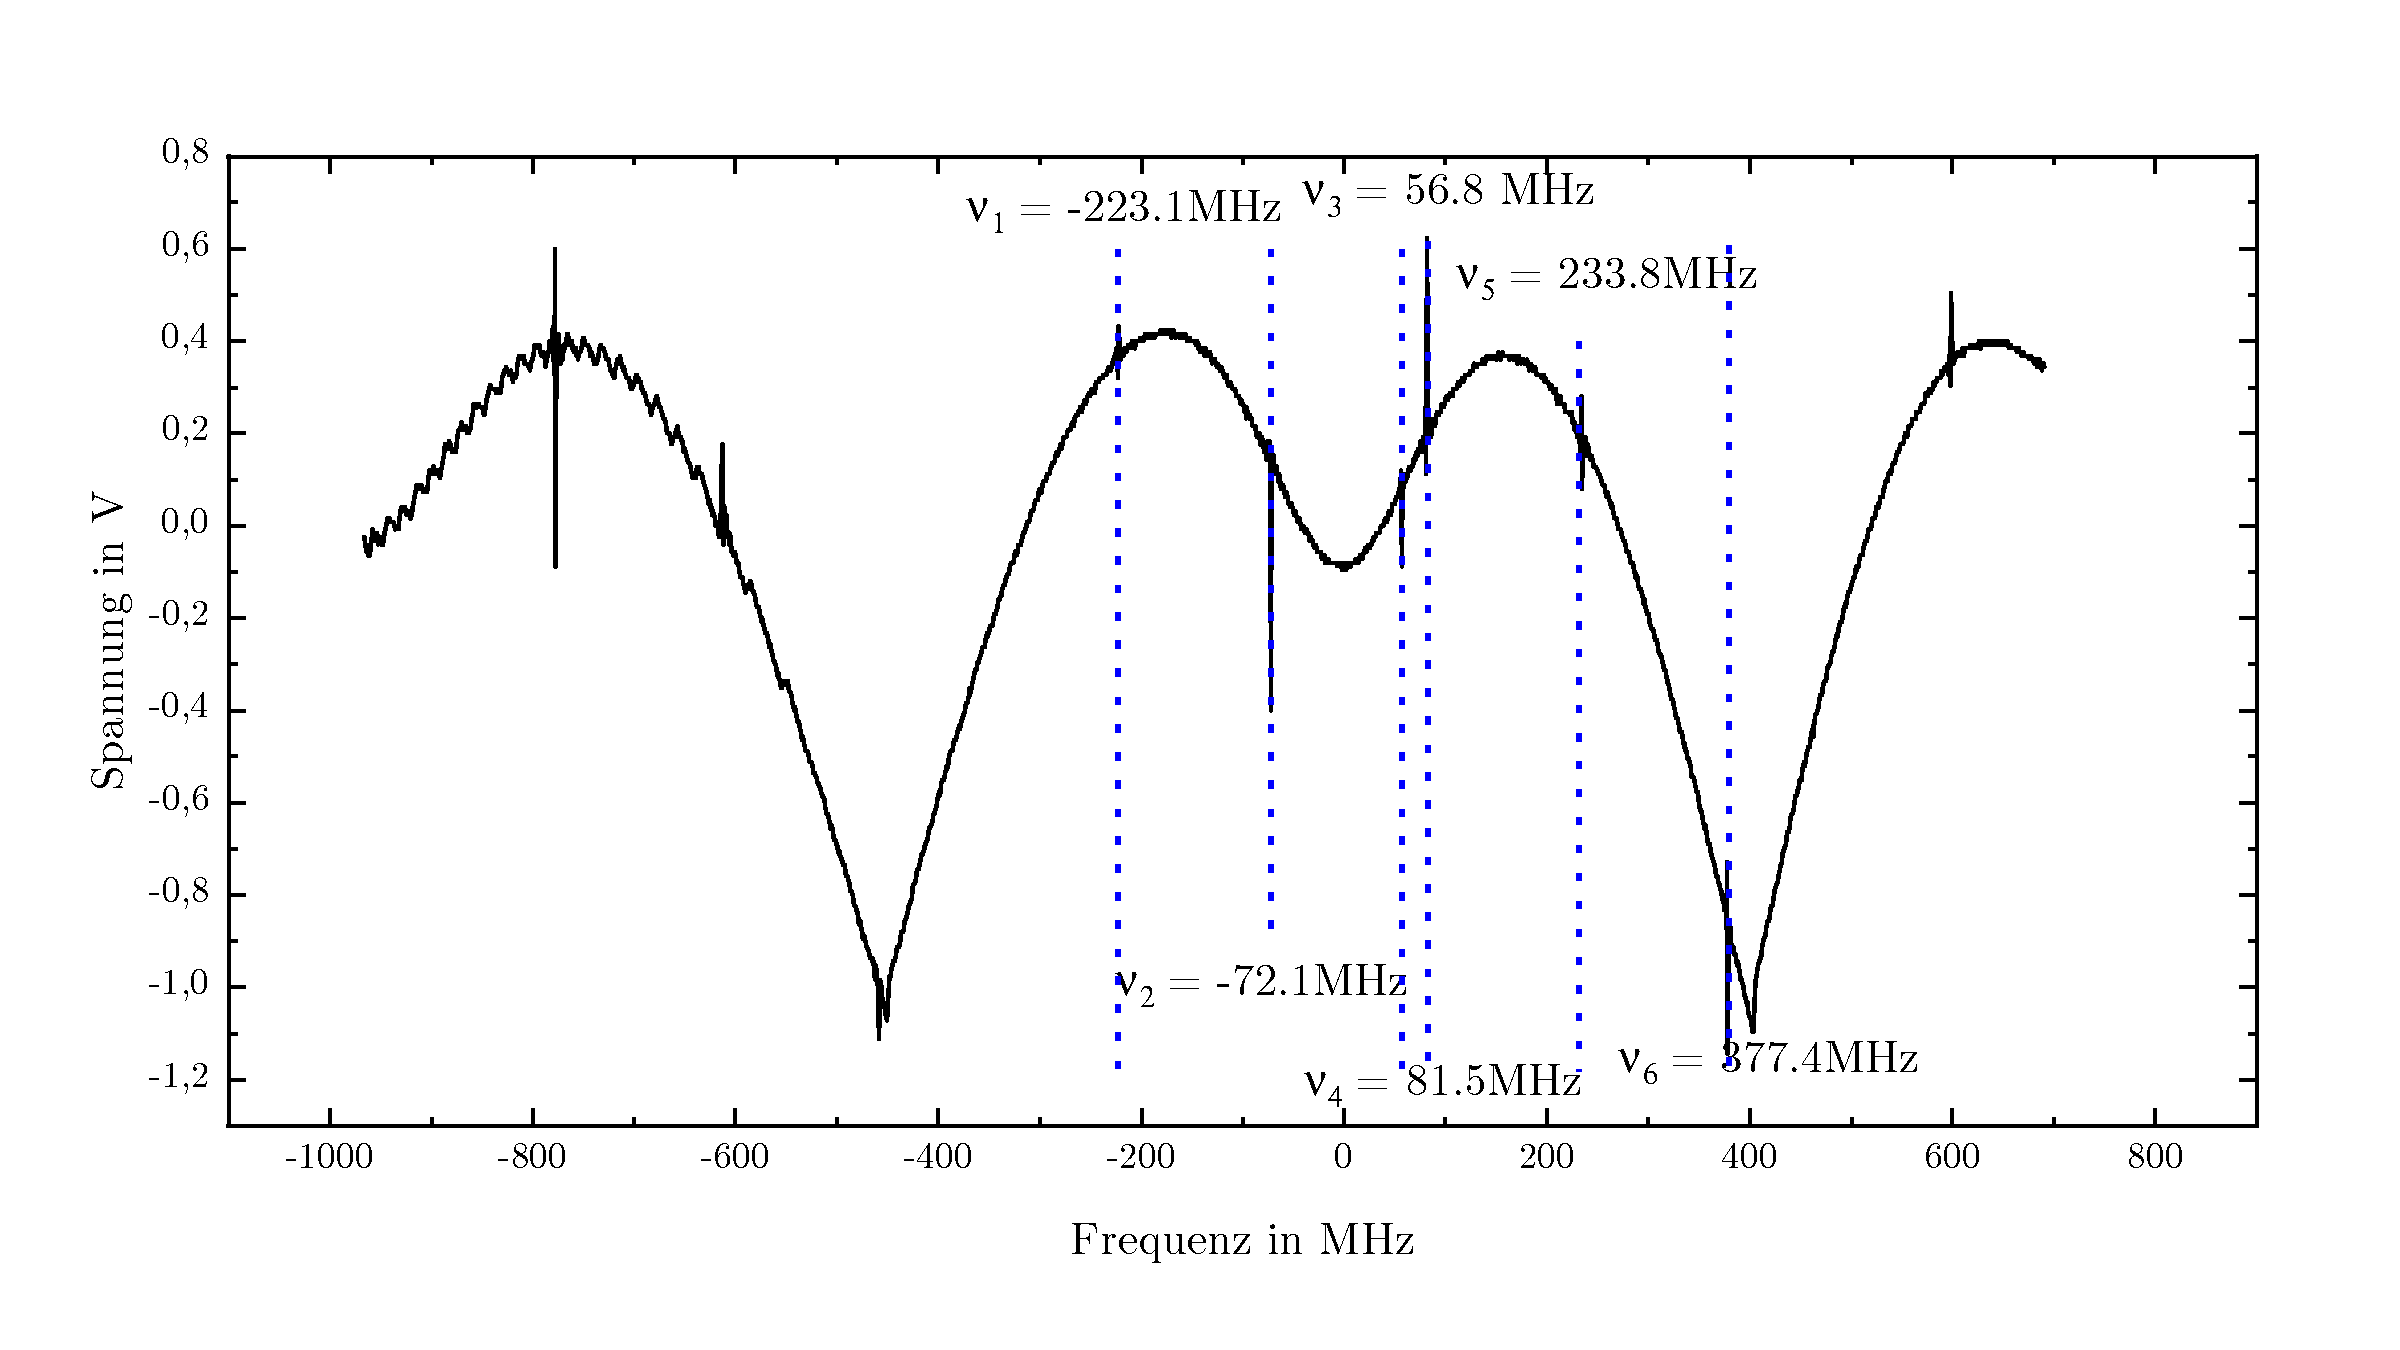
\includegraphics[width=\textwidth]{Bilder/1TransversaleMode_94cm.pdf}
    \caption{erste Transversalmode kann anschwingen}
  \end{subfigure}
  \begin{subfigure}{0.8\textwidth}
    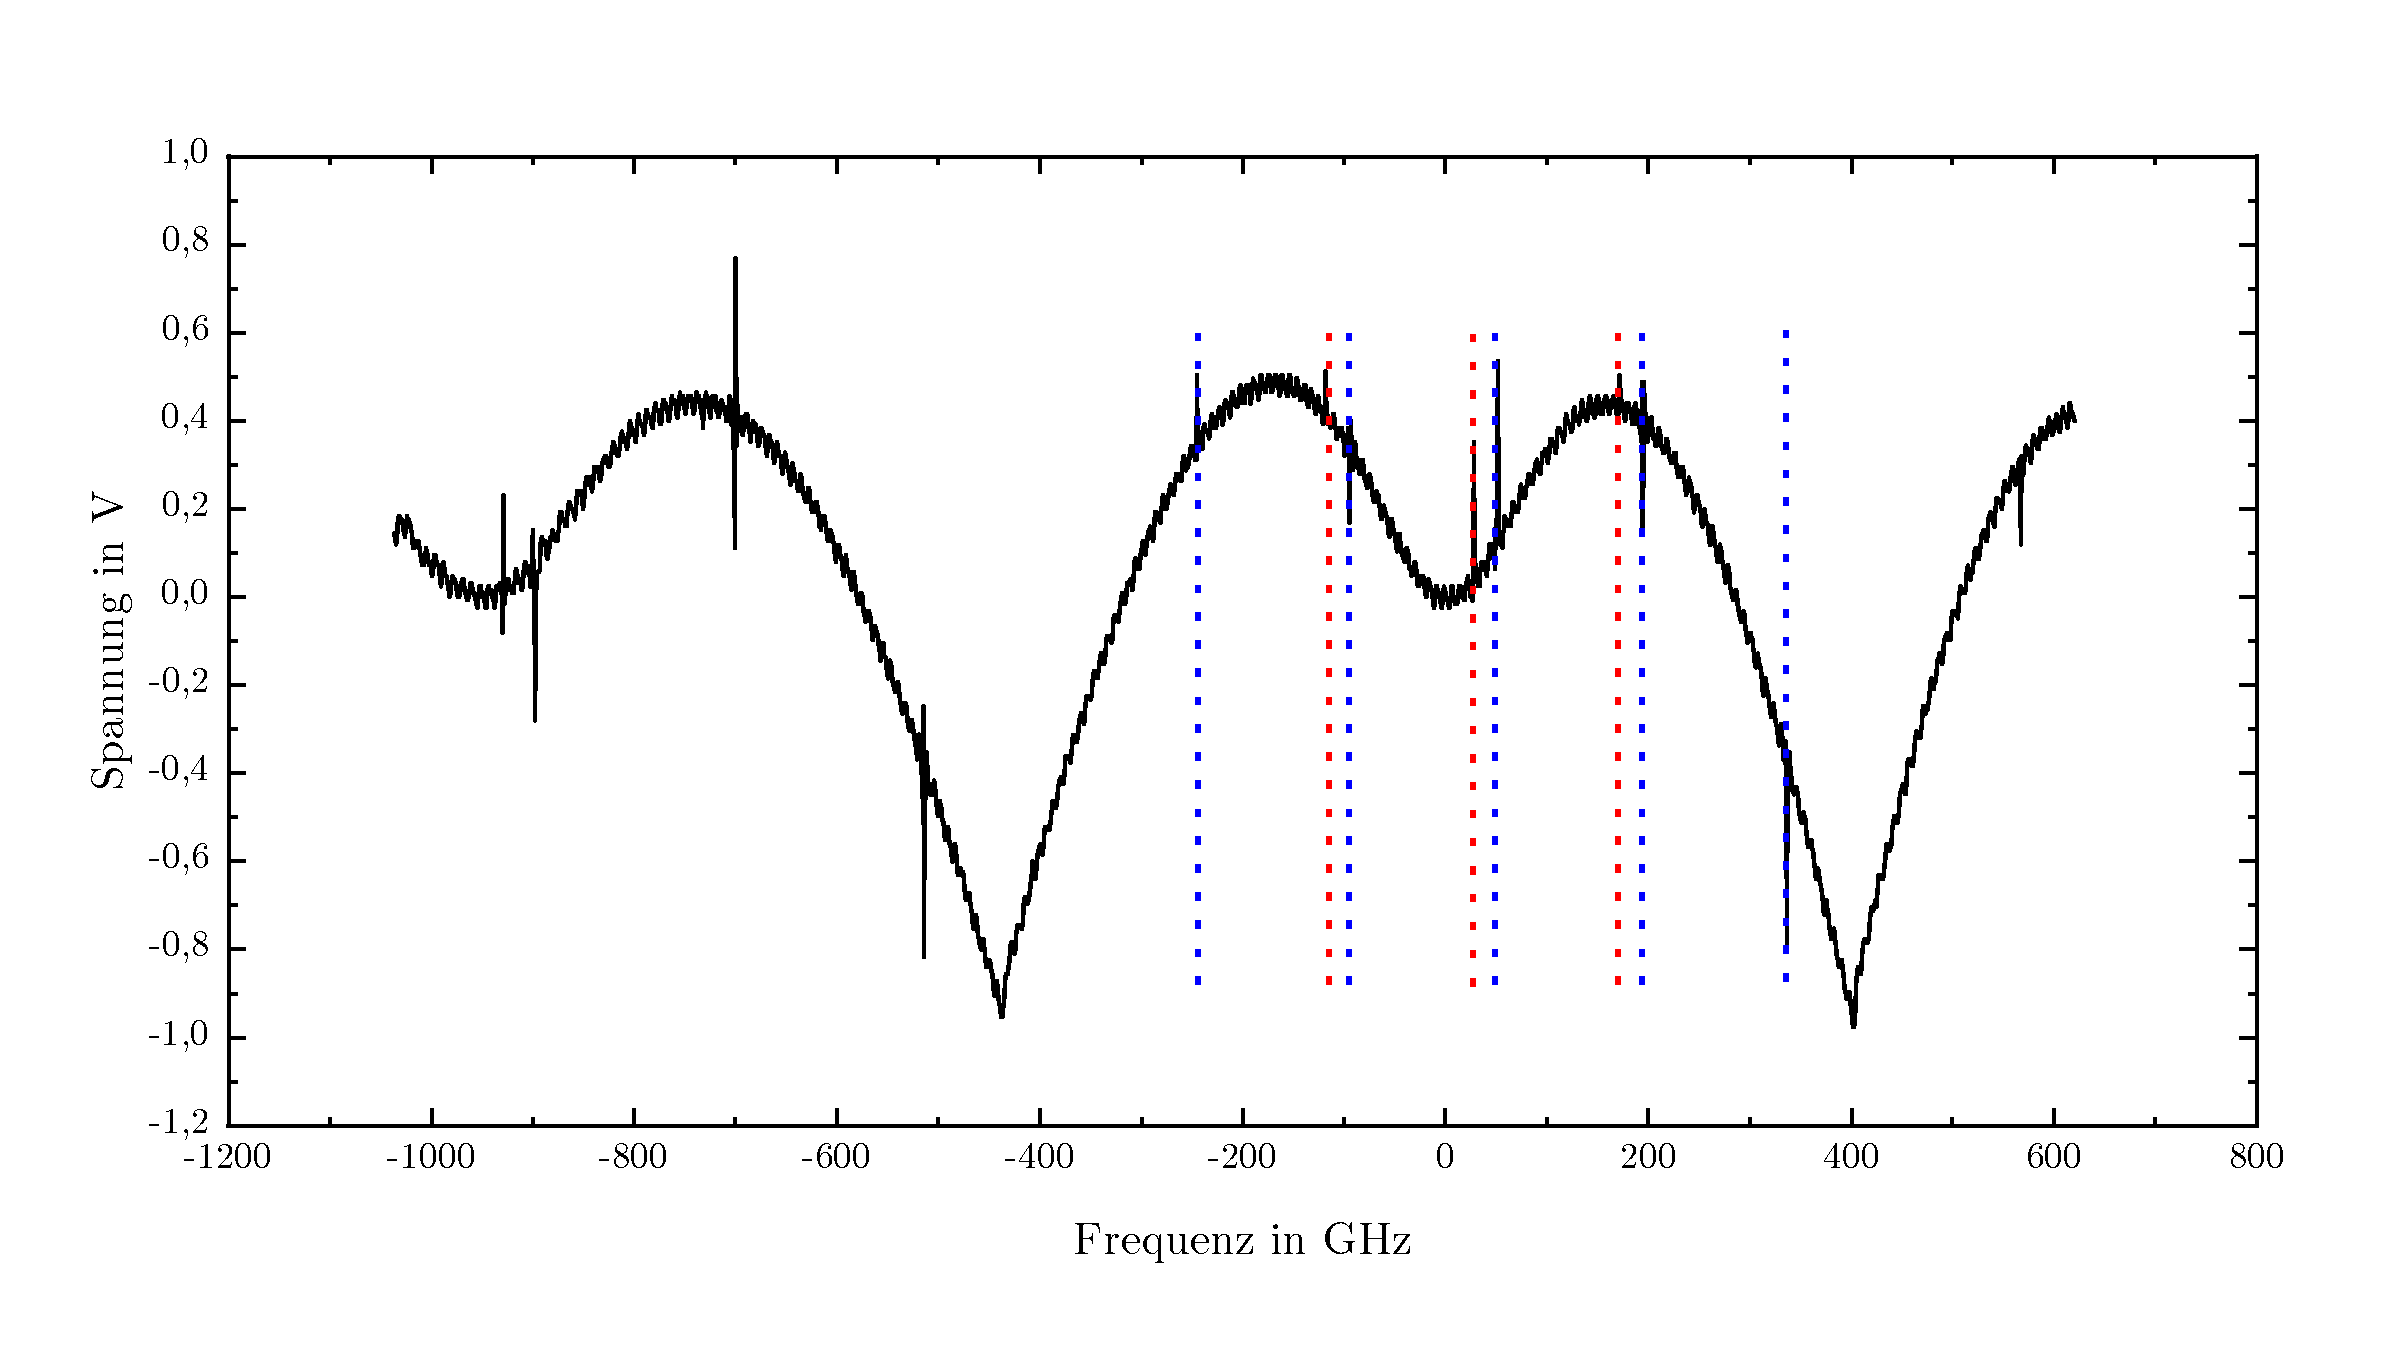
\includegraphics[width=\textwidth]{Bilder/2TransversaleModen_94cm.pdf}
    \caption{erste und zweite Transversalmode kann anschwingen}
  \end{subfigure}
  \caption{Erzeugung von unterschiedlicher Anzahl von Transversalmoden}
  \label{fig:Transversalmoden}
\end{figure}
\FloatBarrier

%
Anhand der folgenden Messung, welche in Abbildung \ref{fig:berührung} zu sehen ist, wird die Empfindlichkeit des Aufbaus deutlich. Bereits eine leichte Berührung des Aufbaus des MML und infolge dessen eine kleine Längenänderung des Resonators auftritt, drückt sich im gemessenen Signal aus. Das bedeutet, dass bereits Längenänderungen im Nanometerbereich mit der Messanordnung vermessen werden können. In der Messung wurde eine Resonatorlänge von \SI{50}{\centi\meter} verwendet und die Irisblende so eingestellt, dass nur eine transversale Mode anschwingen kann.

\begin{figure}[htp]
  \centering
  \begin{subfigure}{0.8\textwidth}
    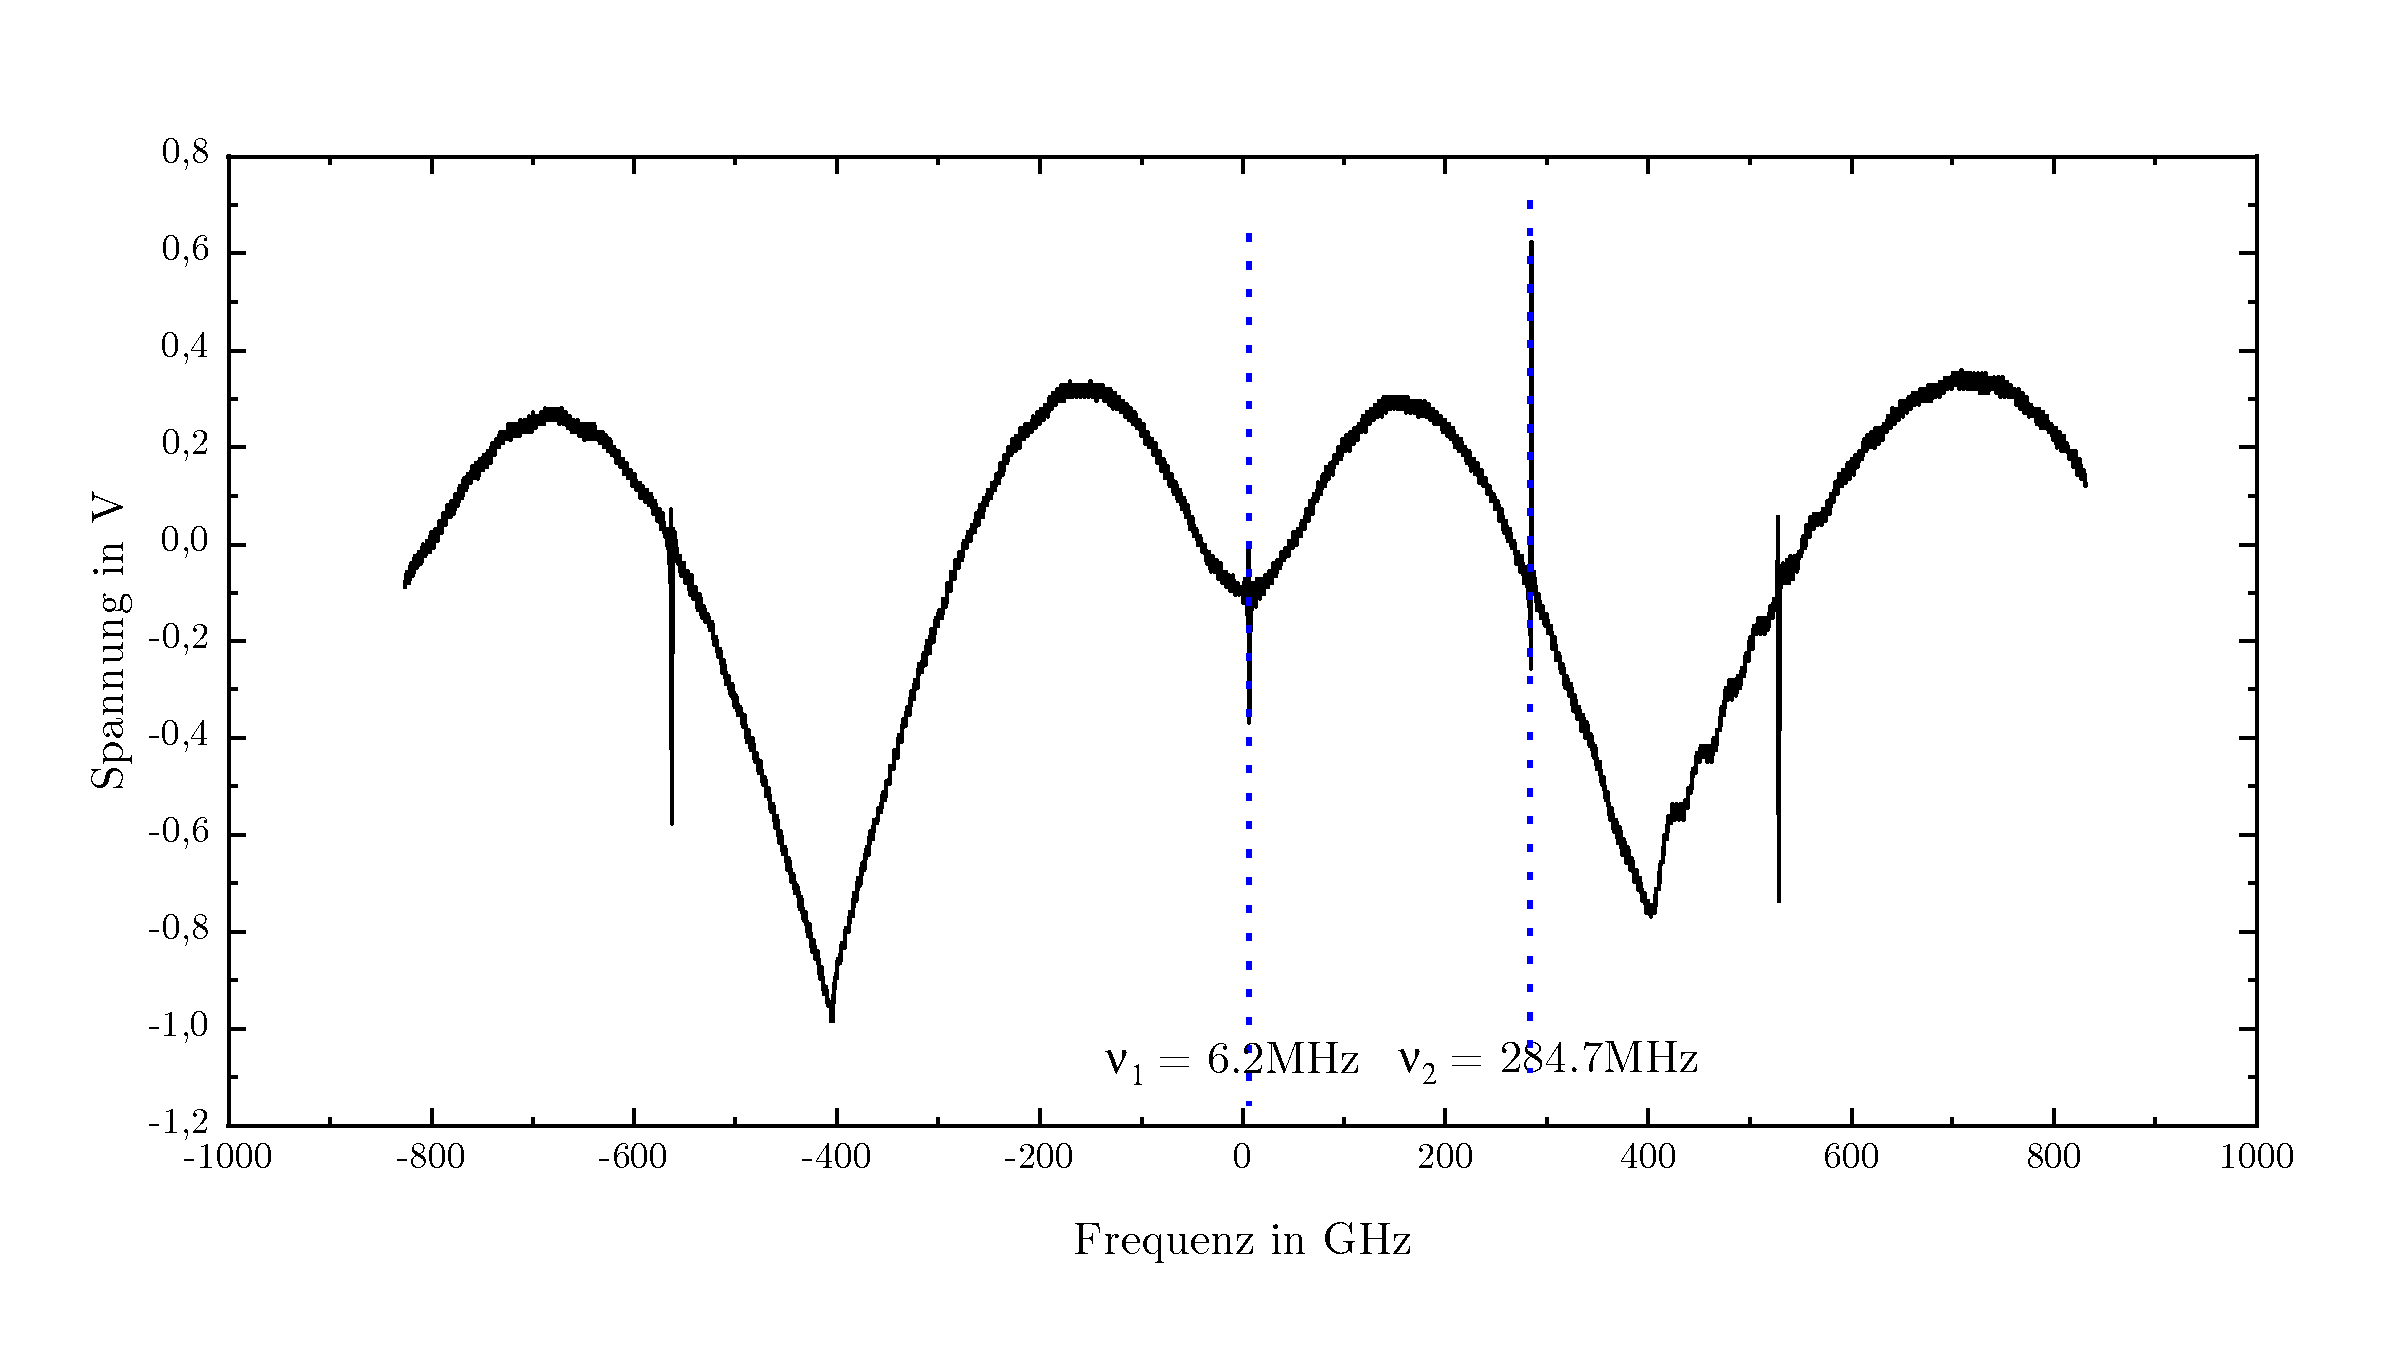
\includegraphics[width=\textwidth]{Bilder/ungedrueckt_50cm_1Mode.pdf}
    \caption{ohne Druck auf Halterung des Aufbaus}
  \end{subfigure}
  \begin{subfigure}{0.8\textwidth}
    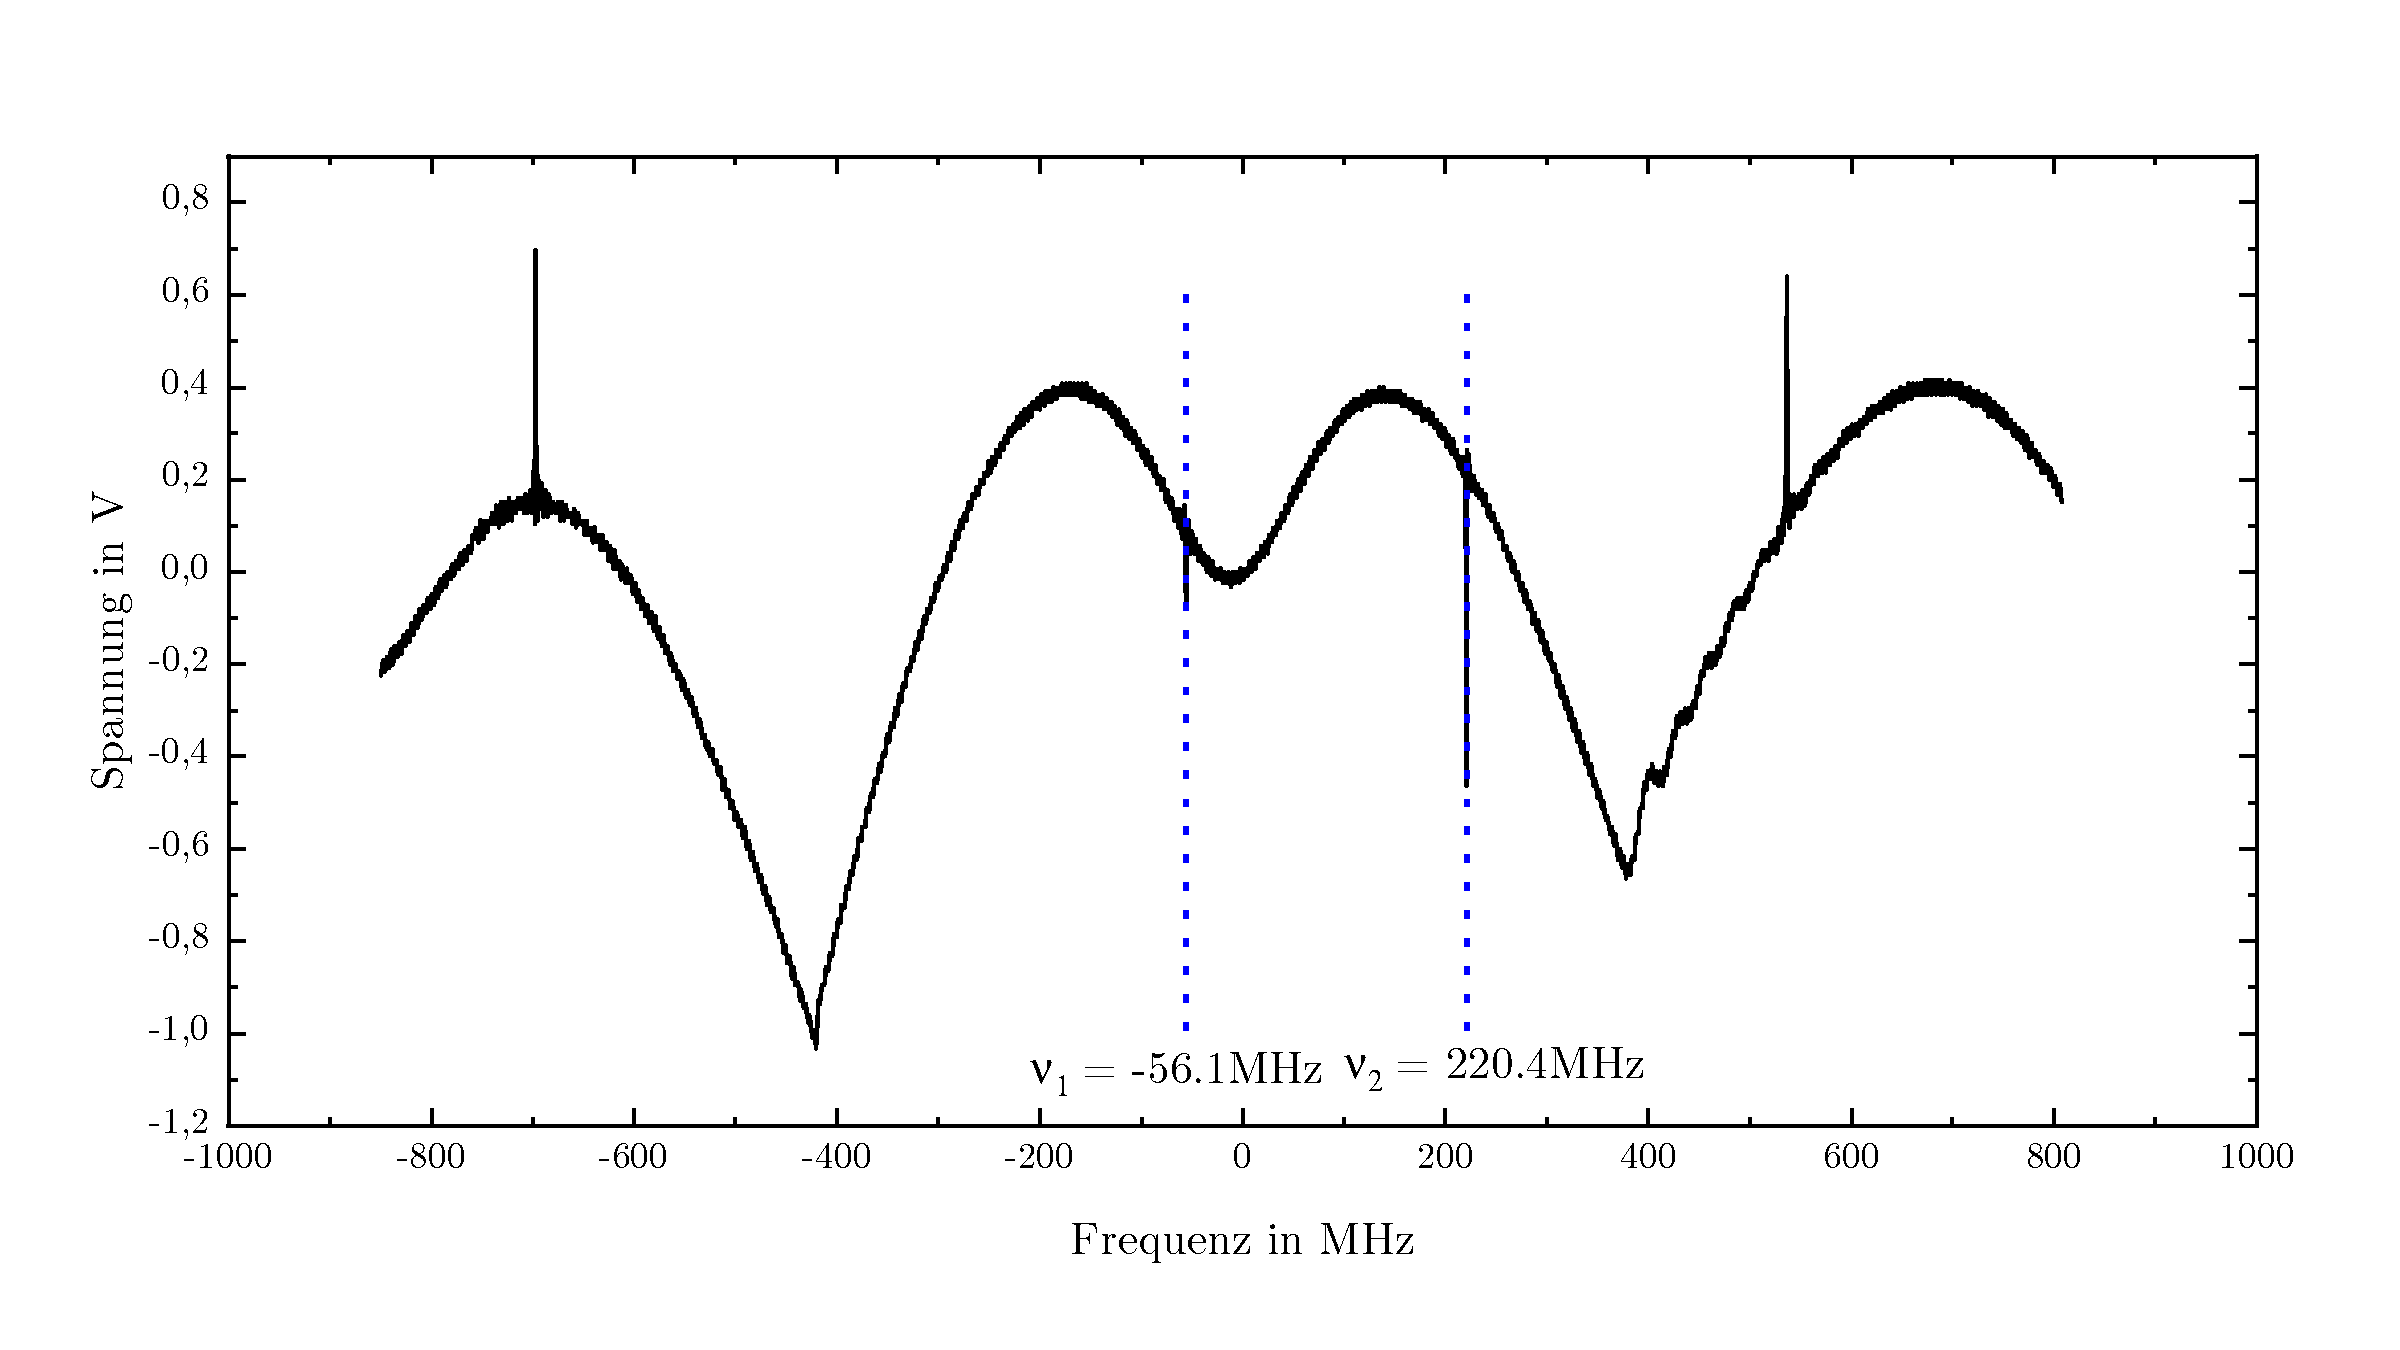
\includegraphics[width=\textwidth]{Bilder/gedrueckt_50cm_1Mode.pdf}
    \caption{mit Druck auf Halterung des Aufbaus}
  \end{subfigure}
  \caption{Frequenzspektrum der Überlagerung der beiden Signal mit und ohne leichten Druck auf den Aufbau}
  \label{fig:berührung}
\end{figure}


\subsubsection{Kurzzeitfluktuationen}
Um die Kurzzeitfluktuationen der Laserfrequenz zu untersuchen wird das Schwebungssignal zwischen den Frequenzen beider Laser in Echtzeit, d.\,h. ohne Wobbelung des Singlemodelasers eingestellt. Dazu überlagern sich beide Laser weiterhin, das Spannungssignal, dass beim Singlemodelaser für die Länge des Resonators sorgt, ist jetzt jedoch nicht mehr als Dreiecksspannung, sondern als konstante Offsetspannung eingestellt, die so gewählt wird, dass die Frequenzen beider Laser sich nur minimal unterscheiden. Es kommt zu einer Schwebung, die in Abbildung~\ref{fig:Schwebung} zu sehen ist.

\begin{figure}[htp]
    \centering
        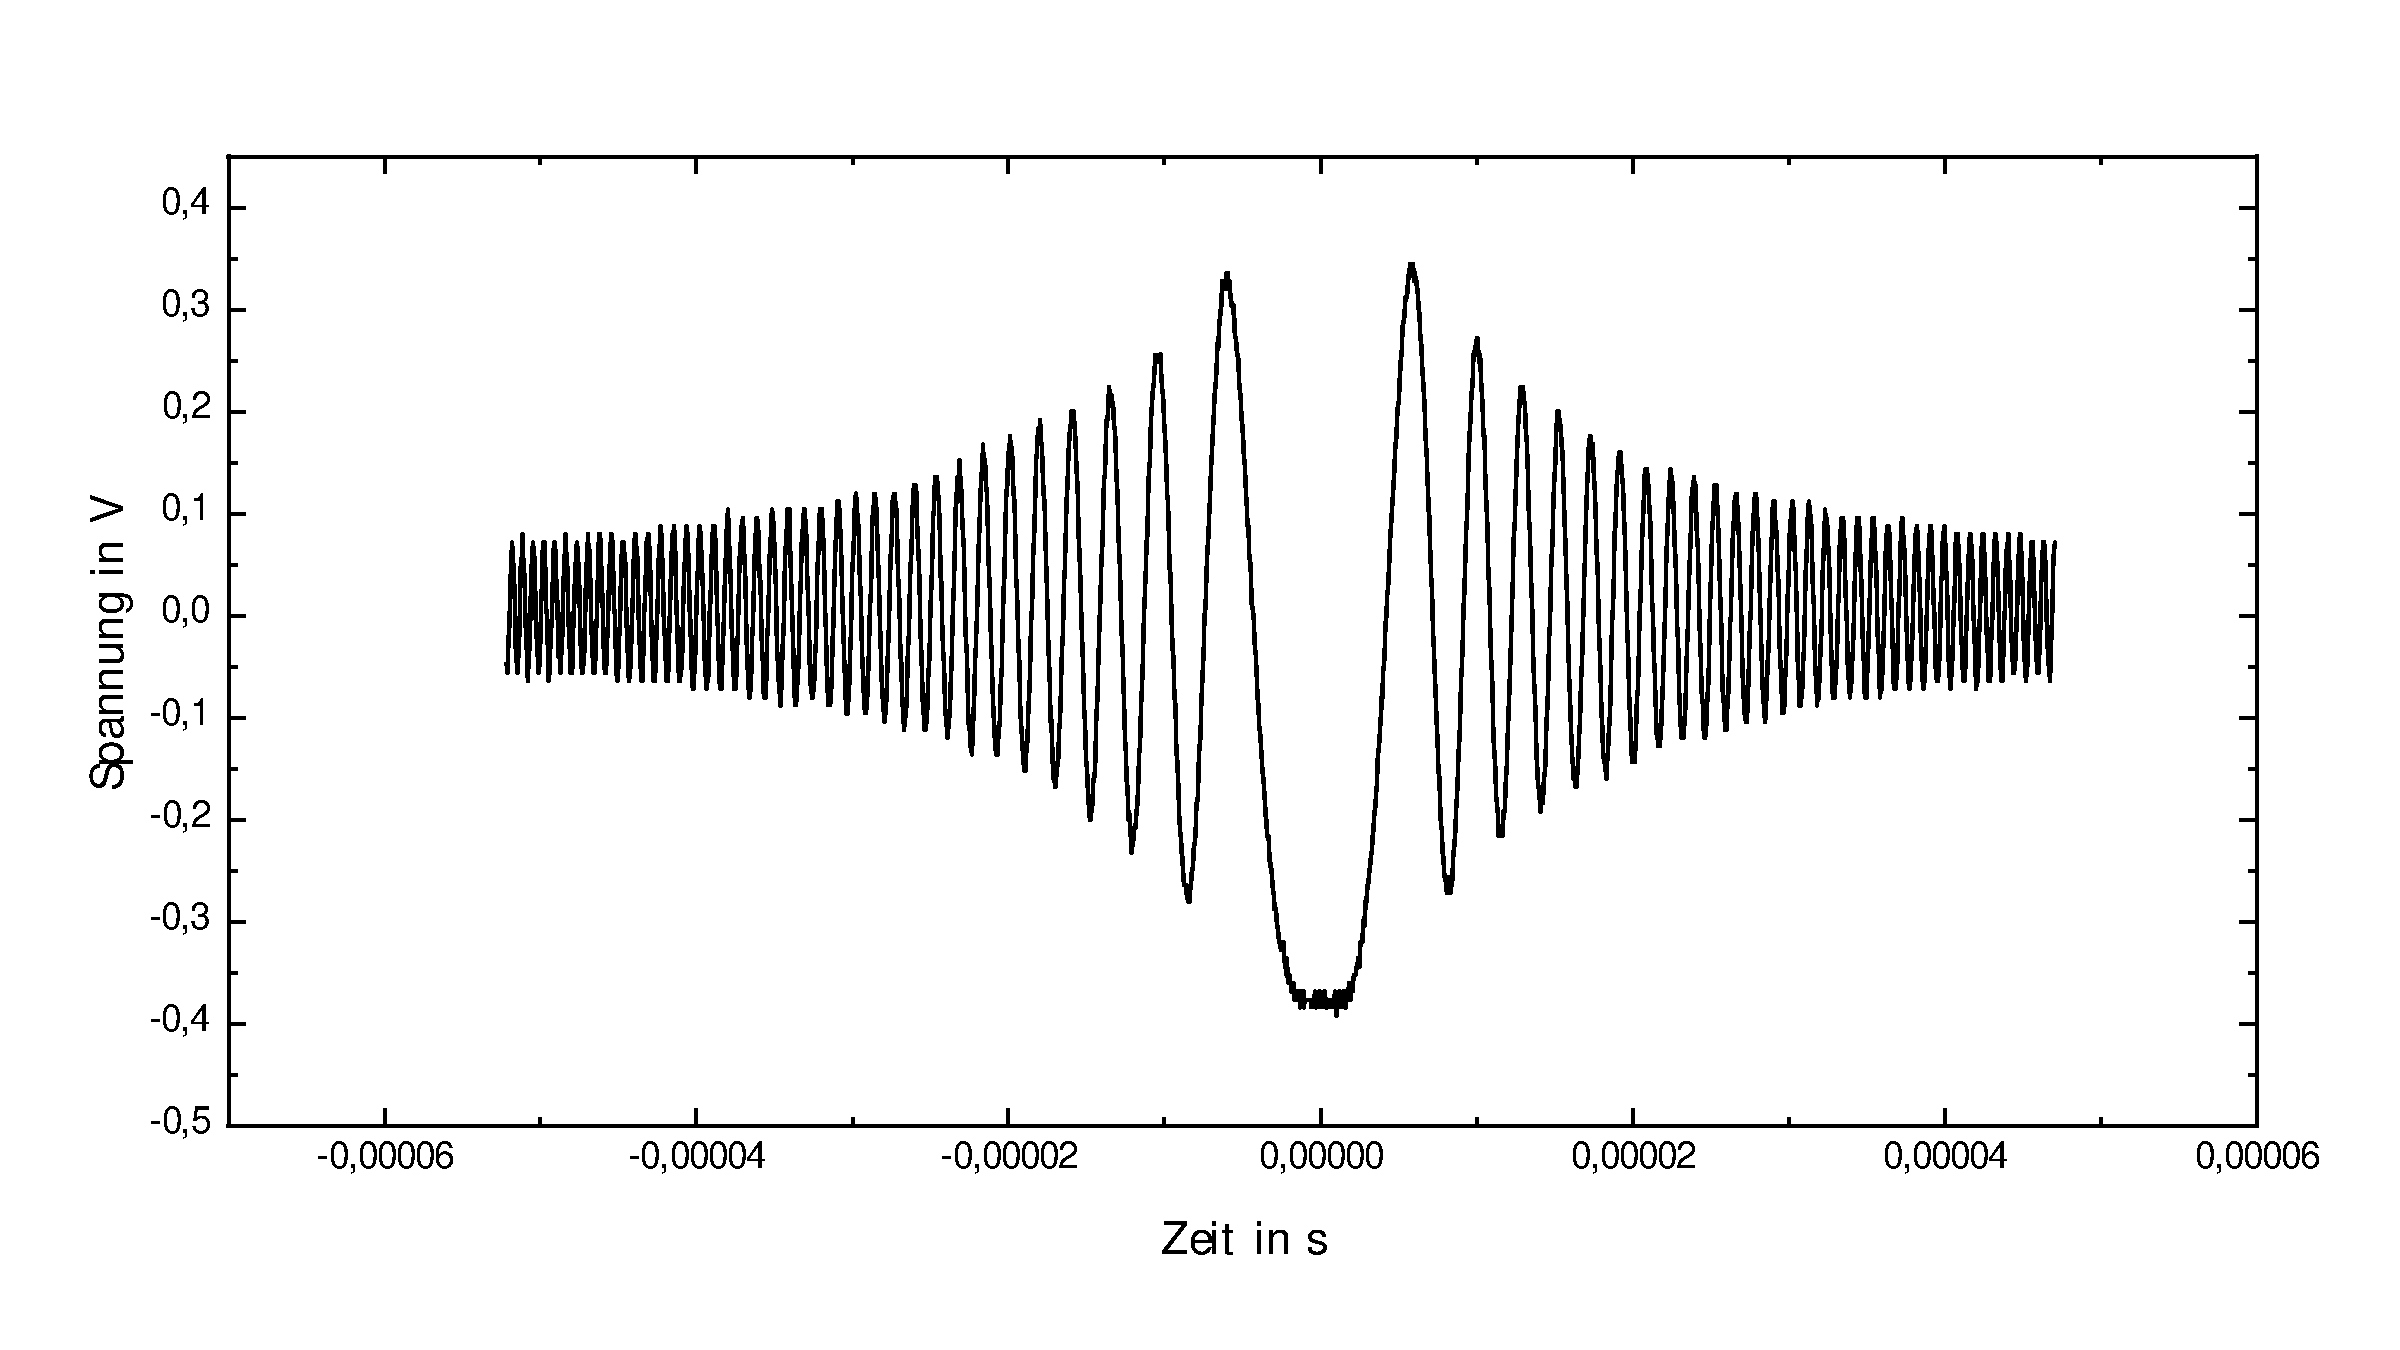
\includegraphics[width=1\textwidth]{Bilder/Schwebungssignal.pdf}
    \caption{Schwebungssignal des Single- und des Multimodelasers}
    \label{fig:Schwebung}
\end{figure}

Anhand dieser lassen sich deutlich die Kurzzeitfluktuationen in der Frequenz des Laser erkennen. Zu sehen ist hier die Intensität, die abhängig ist von der Differenzfrequenz. Wird davon ausgegangen, dass der Referenzlaser nahezu fluktuationsfrei ist, ergeben sich die sichtbaren Änderungen der Frequenz also aus einer Frequenzfluktuation des Singlemodelasers. Eine Größenordnung der Kurzzeitfluktuationen ergibt sich, indem immer zwischen zwei gleichen Minima die Zeitdifferenz und damit die Periodendauer T bestimmt wird und diese der Zeit des rechten Minimas zugeordnet wird. Damit ergibt sich die Gerade in Abbildung \ref{fig: Kurzzeitfluktuationen} aus der die Größenordnung der Kurzzeitfluktuationen auf \SI{0,015}{\mega\hertz\per\micro\meter} bestimmt werden kann.

\begin{figure}[htp]
    \centering
        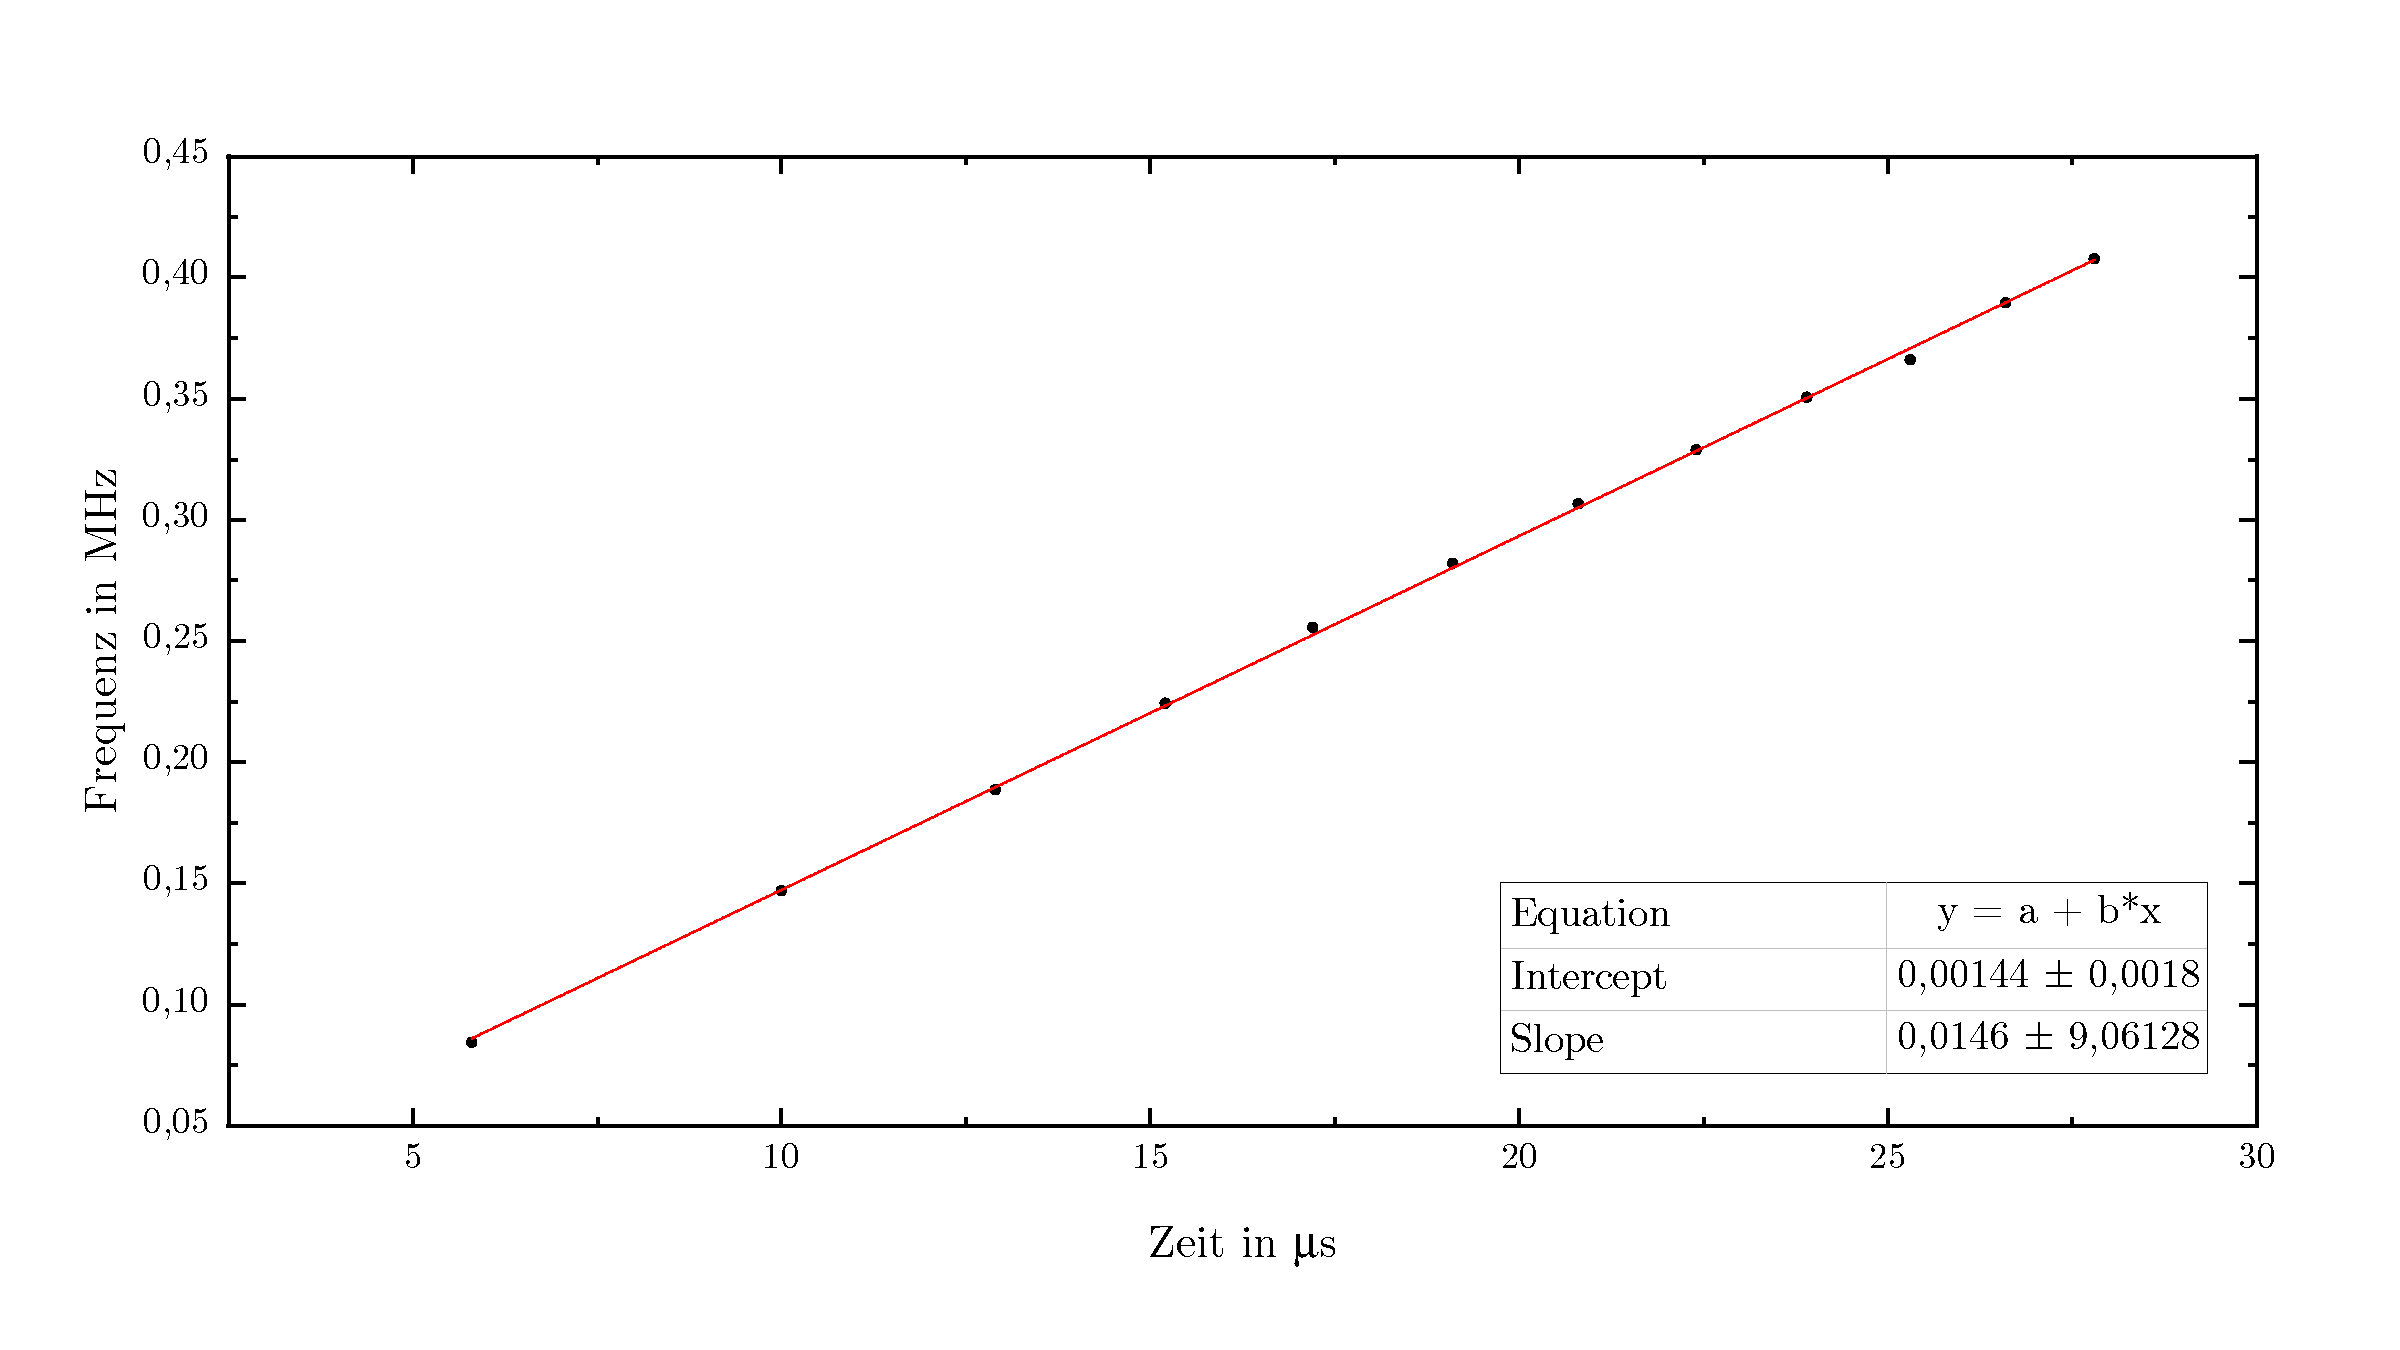
\includegraphics[width=1\textwidth]{Bilder/Kurzzeitfluktuationen.pdf}
    \caption{Kurzzeitfrequenzflukuationen in Abhängigkeit der Zeit}
      \label{fig:Kurzzeitfluktuationen}
\end{figure}

Des Weiteren wird auch makroskopisch ein charakteristischer Verlauf deutlich. Wird das Signal auf etwas größeren Zeitskalen betrachtet, fällt das Anschwingen der Schwebungen im regelmäßigem Bild auf. Jeweils in ein kürzerer und ein längerer Abstand wechseln sich ab. Die Erklärung dafür ist die \SI{50}{\hertz} Netzfrequenz bzw. eine Oberschwingung dieser.

\begin{figure}[htp]
    \centering
        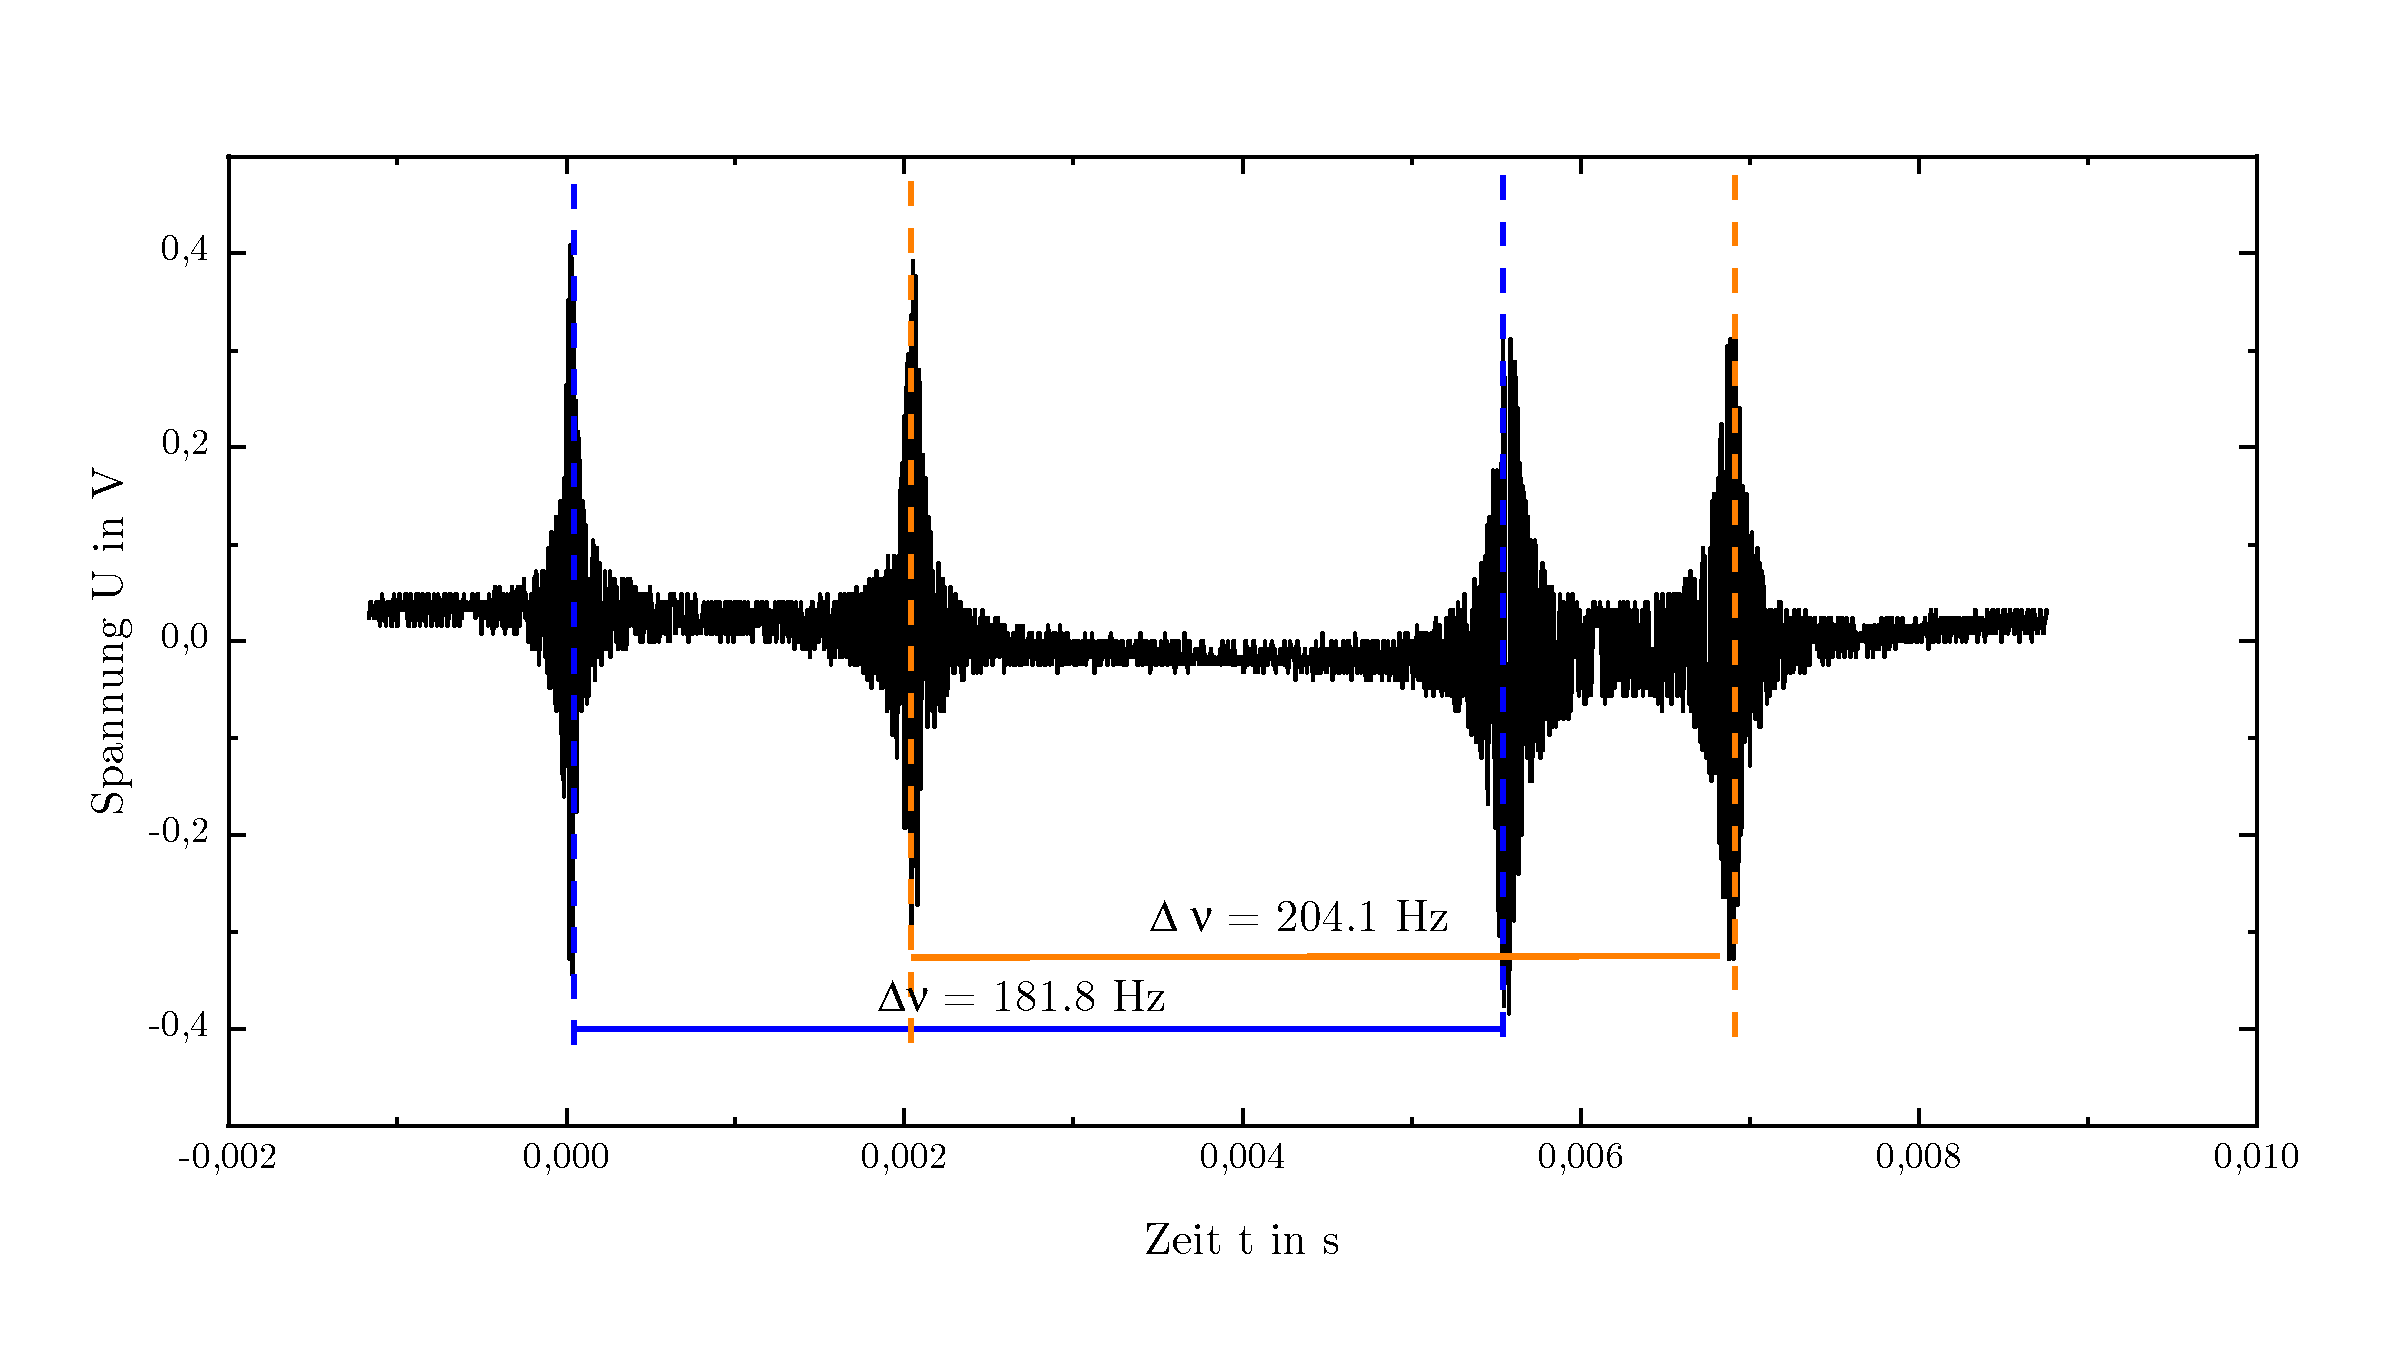
\includegraphics[width=1\textwidth]{Bilder/Fluktuationen_makroskopisch.pdf}
    \caption{Schwebungssignal auf größeren Zeitabständen}
    \label{fig:Schwebungssignal_makro}
\end{figure}

% *********************************************
% ***** KAPITEL 5 *****************************
% *********************************************
\newpage
\section{Zusammenfassung}
Im Versuch konnten die Grundlagen, die Grundprinzipien und die charakteristischen Eigenschaften des Laser nachvollzogen und nachgemessen werden. So konnten durch unterschiedliche Platzierungen eines dünnen Drahtes unterschiedliche Transversal- sowie durch Variation der Resonatorlänge unterschiedliche Longitudinalmoden erzwungen werden, mit Hilfe der $TEM_02$ Mode, die Strahltaille innerhalb und außerhalb bestimmt sowie die Laserleistungen vermessen werden. Außerdem wurde der Wobbelungsbetrieb eines Lasers zur Aufnahme des Laserspektrums erforscht und anhand dessen charakteristische Größen wie die natürliche Linienbreite bestimmt. Durch Überlagerung eines Singlemodelaser und eines Multimodelasers, also Bildung eines optischen Heterodyns, konnten die Position der Moden letzteren bestimmt werden und daran deutlich die Veränderungen bei Längenänderungen beobachtet werden. Dessen Bedeutung als präzises Längenmessungsinstrument wurde deutlich. Außerdem konnten Kurzzeitfluktuationen des Lasers vermessen werden.

\appendix
\section{Fresnel Formeln dielektrischer Medien}
Im Folgenden wird die Bedeutung der \textsc{Fresnel}'schen Formeln für die Reflexion an Grenzflächen verdeutlicht. Für ideale dielektrische Medien ist der Absorptionskoeffizient $\kappa$ des komplexen Brechungsindex gleich Null. Auf beiden Seiten der Grenzfläche wird elektromagnetische Strahlung nicht absorbiert. Damit vereinfachen sich die \textsc{Fresnel}'schen Formeln und es gilt für den Transmissionsfaktor $r$ und Reflexionsfaktor $t$~\cite{Demtroeder2}
\begin{itemize}
  \item \emph{Senkrechte Polarisation} (TE)
  \begin{align}
    \qty(\frac{E_t}{E_e})_s &= t_s = \frac{2 n_1 \cos \alpha}{n_1 \cos\alpha + n_2 \cos \beta}\\
    \qty(\frac{E_r}{E_e})_s &= r_s = \frac{n_1 \cos\alpha - n_2 \cos\beta}{n_1 \cos\alpha + n_2 \cos \beta} = -\frac{\sin(\alpha -\beta)}{\sin(\alpha + \beta)}
  \end{align}
  \item \emph{Parallele Polarisation} (TM)
  \begin{align}
    \qty(\frac{E_t}{E_e})_p &= t_p = \frac{2 n_1 \cos \alpha}{n_2 \cos\alpha + n_1 \cos \beta}\\
    \qty(\frac{E_r}{E_e})_p &= r_p = \frac{n_2 \cos\alpha - n_1 \cos\beta}{n_2 \cos\alpha + n_1 \cos \beta} = -\frac{\tan(\alpha -\beta)}{\tan(\alpha + \beta)}.\label{eqn:Parallele_Polarisation}
  \end{align}
\end{itemize}
Dabei beschreibt $E$ jeweils die Amplitude des elektrischen Feldes. $\alpha$ bezeichnet den Einfallswinkel des Strahls, welcher am Übergang von $n_1$ zu $n_2$ unter dem Winkel $\beta$ gebrochen wird.
Es wird dabei zwischen transversal (TE) und parallel polarisierten Strahlen (TM) bezüglich der Reflexionsebene unterschieden. Die Reflektivität (reflektierte Intensität) ergibt sich aus dem Quadrat des Reflexionsfaktors, analog ergibt sich die Transmissivität. Die Reflektivität von Quarzglas mit einer Brechzahl $n = 1.5$ zeigt Abbildung~\ref{fig:Reflektivität_Fresnel}

\input{Bilder/Reflektivität_Fresnel.tex}

Für den Spezialfall des senkrechten Einfalls gilt $\alpha = \beta = 0$. Hier vereinfachen sich die Formeln für die Reflektivität und es ergibt sich
\begin{align}
  R = \qty(\frac{n_1-n_2}{n_1 + n_2}) = \SI{3.5}{\percent}.
\end{align}
Das entspricht der bekannten Reflektivität von Glas. Für senkrecht polarisiertes Licht ergibt sich nach Gleichung~\eqref{eqn:Parallele_Polarisation} eine Nullstelle für $\alpha + \beta =\SI{90}{\degree}$. Dieser Winkel entspricht dem \textsc{Brewster}-Winkel $\varphi_\text{Brewst.}$, welcher für Quarzglas \SI{56.31}{\degree}. Die parallele Komponente des Strahls wird nicht mehr reflektiert. Im Helium-Neon-Laser, welcher im Praktikum verwendet wird, wird dieser Effekt benutzt, um die auftretenden Reflexionsverluste zu minimieren. Dafür wird das Ende der mit dem aktiven Medium gefüllten Glaskapillare geneigt (Brewsterfenster). Zusätzlich kann damit sichergestellt werden, dass das Laserlicht parallel polarisiert ist.

% ***** Literaturverzeichnis ******************

\bibliography{Literatur}{}
\bibliographystyle{plain}
\end{document}
